\documentclass[11pt, a4paper, English]{report}
\usepackage{calc}
\usepackage{graphicx} % Pour gérer les figures
\usepackage{wrapfig}
\usepackage{cancel}%pour barrer des éléments
\usepackage{array,multirow,makecell}
\usepackage{xcolor,graphicx}
\setcellgapes{1pt}
\makegapedcells
\newcolumntype{R}[1]{>{\raggedleft\arraybackslash }b{#1}}
\newcolumntype{L}[1]{>{\raggedright\arraybackslash }b{#1}}
\newcolumntype{C}[1]{>{\centering\arraybackslash }b{#1}}
\usepackage{times} % Pour choisir la police de caractère (choix limité)
\usepackage{hyperref}
 \usepackage{multirow}
\usepackage{amsfonts, amsmath, amssymb} %maths
\usepackage{fancyhdr}
\usepackage{appendix}
\usepackage[utf8]{inputenc}
% Vous trouverez ces infos dans le site http://www.commentcamarche.net/contents/latex/latex-entete.php3 par exemple. Il y en a un très grand nombre. Penser à choisir une doc et vous y tenir car sinon on perd du temps.

\usepackage[T1]{fontenc} % permet de spécifier à LaTeX l'utilisation du codage de caractères T1, nouvelle norme LaTeX non utilisée par défaut pour des raisons de compatibilité avec les anciens documents LaTeX.

\usepackage[english]{babel} %permet l'adaptation de LaTeX au français. En particulier, la table des matières du document est appelée "table des matières" et non "table of contents". Lors de la compilation, LaTeX convertit les caractères accentués en caractères unicodes (ensemble normalisé et universel de caractères).

\RequirePackage{geometry} % Régler la taille de la page

\usepackage{eurosym} % Pour faire \euro qui donne ?

\usepackage{color}

\geometry{a4paper, %wesh poto
width=16cm,
height=24cm,
headsep=1.5cm,
headheight=15pt,
footskip=2cm}% Format de la page. On décide. Il faut regarder la doc.
\widowpenalty=10000
\clubpenalty=10000
\hyphenpenalty=5000
\tolerance=1000
\textwidth = 16cm
\linewidth = 16cm % Cela permet d'avoir une variable que l'on utilise (voir plus bas).

\parindent=0cm % Indenter la 1re ligne de chaque paragraphe.
\setlength{\parindent}{0cm}
%\setlength{\parskip}{1ex plus 0.5ex minus 0.2ex}
\newcommand{\hsp}{\hspace{20pt}}
\newcommand{\HRule}{\rule{\linewidth}{0.5mm}}

\begin{document}

\begin{titlepage}
% \pagecolor{blue!10}
\begin{center}
	\begin{minipage}{2.5cm}
	\begin{center}
		
\includegraphics[width=3.3cm,height=1.7cm]{logo.png}
		
	\end{center}
\end{minipage}\hfill
\begin{minipage}{10cm}
	\begin{center}
	\textbf{ Sorbonne Université}\\[0.1cm]
    \textbf{Master Sciences pour l'Ingénieur}\\[0.1cm]
    Énergétique et Environnement, parcours Cleaner
% 		\textsc{\uppercase{Université Sultan Moulay Slimane}}
		
% 		\uppercase{éCOLE NATIONALE DES SCIENCES APPLIQUéES KHOURIBGA} 
	\end{center}
\end{minipage}\hfill
\begin{minipage}{2.5cm}
	\begin{center}
		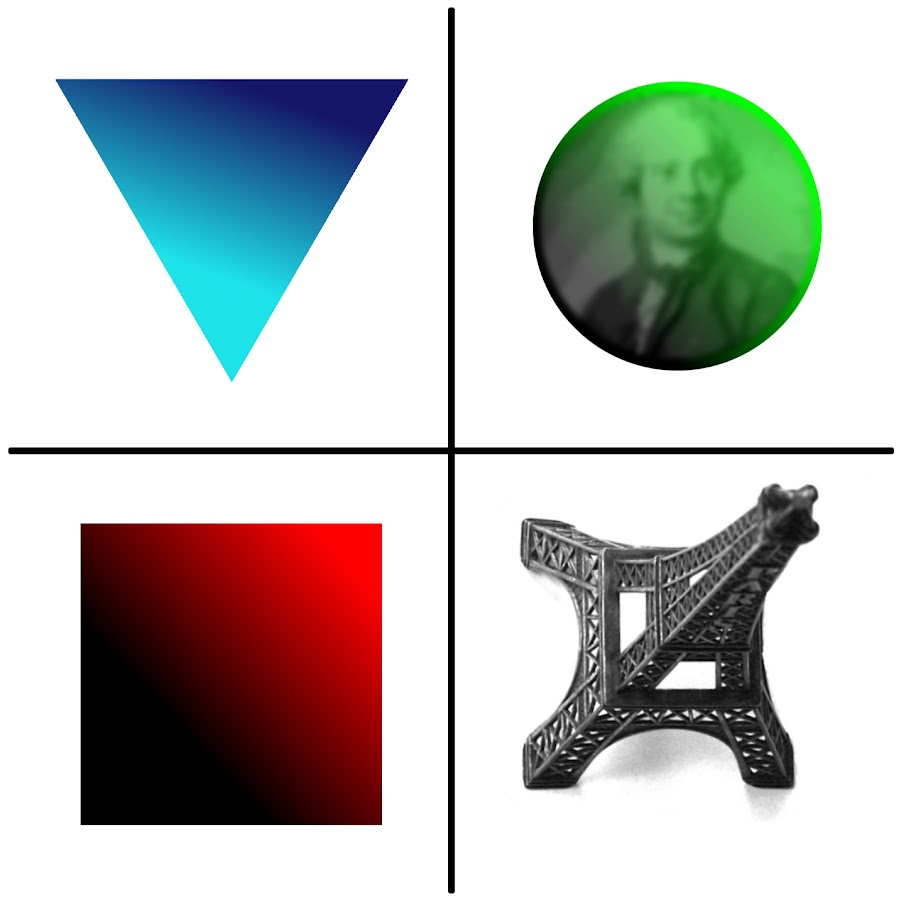
\includegraphics[width=2.4cm,height=2.2cm]{logo2}
	\end{center}

\end{minipage}
%\includegraphics[width=0.6\textwidth]{logo-isae-supaero}\\[1cm]
\textsc{\Large }\\[6cm]
{\Large \bfseries MSc End-of-studies internship report}\\[0.5cm]



% Title
\rule{\linewidth}{0.3mm} \\[0.4cm]
{ \huge \bfseries\color{blue!40!black} Development of a forward-backward numerical uncertainties propagation tool \\[0.4cm] }
\rule{\linewidth}{0.3mm} \\[1cm]
{\large \bfseries Institut Jean le Rond $\partial$'Alembert (IJLRDA)}\\[3cm]
% \includegraphics[width=0.3\textwidth]{logo-isae-supaero}\\[1cm]
% Author and supervisor
\noindent
\begin{minipage}{0.4\textwidth}
  \begin{flushleft} \large
    \emph{\color{red!40!black}Author :}\\
    Hector \textsc{Galante Amino}\\
  \end{flushleft}
\end{minipage}%
\begin{minipage}{0.5\textwidth}
  \begin{flushright} \large
    \emph{\color{red!40!black}Supervisors:} \\
    Anca \textsc{Belme} (IJLRDA)\\
    Jean-Camille \textsc{Chassaing} (IJLRDA)\\
  \end{flushright}
\end{minipage}\\[2cm]

\color{blue!40!black}{\large \textit{Presented on the $19^{th}$ of september for the following jury : }}\\[0.3cm]

\color{black}
\centering
\begin{tabular}{ll}
\large Phillipe \textsc{Guibert} : & \large IJLRDA \\[0.1cm]
\large Nicolas \textsc{Bertier} : & \large ONERA \\[0.1cm]
\large Daniel \textsc{Gaffie} : & \large ONERA 
\end{tabular}

\vfill

% Bottom of the page
{\large \color{red!40!black}{Academic year}\\ \color{blue!40!black}2018/2019}

\end{center}
\end{titlepage}

\begin{abstract}

This report is made in the context of my internship at the end of my second and last year of my MSc degree at the "Institut Jean le Rond $\partial$'Alembert" laboratory, based in Paris, France. \\
In this five months study, we employ a non intrusive adaptive stochastic collocation method coupled with a consistent Bayesian inference to propagate forward and inverse numerical uncertainties in aerodynamic problems. This tool combines the advantage of not modifying the deterministic computations and to match a distribution in the stochastic domain given a model and a prior density. Its efficiency is evaluated first with analytical examples and then with a flow around a NACA0012 airfoil using the free-stream Mach and angle of attack as the solver uncertain parameters. Finally, we add a combustion parameter to the CFD model in a scramjet configuration. The stochastic collocation forward propagation is shown to be as accurate as MC crude simulations using a smaller number of deterministic evaluations and able to map singularities in the stochastic domain. Moreover, we show that if the number of parameters $\xi$ are equal to the number of interest quantities, the solution to the inverse problems behaves as unique. Possible CFD applications are presented to emphasise the potential of this tool.

\end{abstract}
\begin{abstract}
Ce rapport traite de mon stage de fin d'études pour l'obtention du diplôme Master Sciences pour l'Ingénieur, spécialité Énergétique et Environnement, où j'ai effectué un stage de 5 mois au sein du laboratoire "Institut Jean le Rond $\partial$'Alembert" à Paris.\\
Cette projet de 5 mois a consisté à coupler des propagations inverses et directes d'incertitudes numériques. Une méthode de collocation stochastique adaptative non intrusive a été combinée à une pseudo-inférence Bayésienne dans le but de construire un outil performant et terme de temps de calcul et précision pour l'étude de modèles complexes. L'objectif est d'approcher une distribution d'une certaine quantité d'intêret  à partir d'une distribution à priori et un modèle, sans pour autant modifier les calculs deterministes effectués. L'outil developpé est d'abord testé sur des problèmes analytiques puis pour des problèmes CFD (Naca0012 et scramjet). La collocation stochastique s'est montré aussi précise que des simulations Monte Carlo tout en baissant l'ordre du nombre de calculs deterministes nécéssaires de $10^2$ et en étant capable de détecter des discontinuités dans l'espace stochastique considéré. De plus, nous montrons que si le nombre de quantités d'intêret et paramètres incertains sont égaux, la solution du problème inverse tend à être unique. Enfin, des idées d'applications CFD sont données dans le but de présenter l'important potentiel de cet outil.
\end{abstract}

\renewcommand{\abstractname}{Acknowledgements}
\begin{abstract}
I would like to express my special thanks of gratitude to my supervisors Anca Belme and Jean Camille Chassaing, for their expert advice, patience, and encouragement throughout this project. Having never worked in such numerical field, it has been a pleasure to collaborate with them and I'm grateful for this opportunity and for what I learnt. They	have shown me,	by	his	example,	what	a	good scientific researcher	(and	person)	should	be.\\\\
Secondly, I	am	grateful	to	all	of	those	with	whom	I	have	had	the	pleasure	to	work	during	this project and my colleagues. A special thanks to Mahshid Sharifi for his friendship and his help.
\\\\
Thanks also to Yutao and other interns for their friendship in the lab.
\\\\
Last but not least, I owe my deepest gratitude to my parents and my friends who have supported me along the way.
\end{abstract}
\newpage
\section*{List of abbreviations and symbols}
$\alpha$ : Learning rate. \\
$\delta_j^i$ : Neuron $j$ in a layer $i$ error.\\
$\rho_{IVC}$ : IVC gaz density. \\
$\sigma_i$ : Activation function for a given layer $i$. \\
$a_j^i$ : Value taken by a neuron $j$ in a given layer $i$. \\
ANN : Artificial neural network. \\
\textbf{b} : Biases array.\\
$C$ : Cost function. \\
$CO$ : Carbon monoxide. \\
$CO2$ : Carbon dioxide. \\
$EOC$ : End of combustion. \\
$FANN$ : Fast Artificial Neural Network.
$Fr$ : Air-fuel ratio. \\
$HC$ :  Unburned hydrocarbons. \\
$ID$ : The ignition delay. \\
$IVC$ : Inlet Valve Close. \\
$ma$ : Engine measured air mass flow. \\
MLP : Multi layer perceptron. \\
$MSE$ : Mean square error function. \\
$N$ : Engine speed. \\
NN : Neural network. \\
$NOx$ : Nitrogen oxides. \\
$P_{inj}$ : Pressure of injection. \\
$R$ : Universal ideal gas constant value. \\
$T_{IVC}$ : IVC temperature. \\
$Tw$ : Temperature of water. \\
\textbf{X} : Inputs array. \\
\textbf{Y} : Measured output array. \\
$\hat{Y}$ : Network's output array. \\
$YCO$ : Carbon monoxide mass fraction. \\
$YHC$ : Unburned hydrocarbons mass fraction. \\
$YO_{2IVC}$ : IVC $O_2$ mass fraction. \\
$YSOOT$ : Soot mass fraction.
$w_j$ : Single weight. \\ % a completer
\textbf{W} : Weights array.\\
\color{blue!40!black}{\chapter{Introduction}}
\color{black}
\section*{l'Institut Jean le Rond d'Alembert}
The Jean le Rond d’Alembert Institute was created in 2007, uniting 5 former laboratories (Laboratory of Mechanics Modeling - Laboratoire de Modélisation en Mécanique, Musical Acoustics Laboratory - Laboratoire d’Acoustique Musicale, Laboratory of Physical Mechanics - Laboratoire de Mécanique Physique, Energy and Internal Fluid Mechanics Laboratory - Laboratoire d’Energétique et Mécanique des Fluides Internes, Mechanics, Materials and Structures Laboratory - Laboratoire de Mécanique, Matériaux et Structures). It counts 170 people working in basic and applied research in mechanics. Its main research fields are mechanics, acoustics and energy. Therefore, the laboratory is divided in five teams covering the mechanical fields cited above  : 
\begin{itemize}
    \item Complex Fluids and Hydrodynamic Instabilities (FCIH - Fluides Complexes et Instabilités Hydrodynamiques). Activities in this team are mainly oriented in 5 axis : numerical simulations of droplets and bubbles (Atomization, impact and bubbles dynamics), fluid-solid interactions, vorticity study, the natural/complex environment flows study and in developing numerical tools for fluid mechanics simulations.
    \item Combustion, New Energies and Turbulence (CEPT - Combustion, Energies Propres et Turbulence) which focuses in intern turbulence problems and combustion simulations.
    \item Modeling, Propagation and Acoustic Imaging (MPIA - Modélisation, Propagation et Imagerie Acoustique)
    \item Lutherie, Acoustics, Music (LAM - Lutheries Acoustique Musique)
    \item Mechanics and Engineering of Solids and Structures (MISES - Mécanique et Ingénierie des Solides et des Structures)
\end{itemize}


\section*{Problem contextualisation}
Supervised by Anca Belme (FCIH) and Jean Camille Chassaing (MPIA), my main goal was to build a forward-backward propagation tool for numerical uncertainties. \\\\
With the growing computational power, physical phenomenons simulations are used by every research and development company allowing scientists to save time and model while computing accurate results. To do so, models are used. Nevertheless, no model shall give a single deterministic solution, but something very close to the reality. Thus, quantifying numerical uncertainties allows one user to consider the model parameters' uncertainty impact on a given quantity of interest (QoI) in a given context, raising its model liability. Such studies provide, instead of a single deterministic model output, its distribution in a random, stochastic domain. This kind of study shows up to be computationally expensive, where many calculations in the stochastic domain must be made to have accurate results. Computing a response surface can take a long time, specially for complex solvers such as CFD ones. Thus, many studies aim to reduce the required number of model running to build a given surface. Among the numerous mathematical methods existing to approximate the surrogate model, I had to choose between the Generalised Polynomial Chaos \cite{xiu} and a Stochastic Collocation method \cite{NasaSCM}, developed by J. Van Langenhove during his thesis \cite{Janthesis} which solves a minimisation problem in the Riemann Metric to build an adaptive stochastic mesh \cite{Loseille}\cite{Loseillemesh}. \\\\
After reducing the number of computations needed we seek to couple the forward propagation with the Consistent Bayesian Inference method presented by Butler et al \cite{Tim2}, which combines various aspects of both Bayesian inferences \cite{RSampling} and measure-theoretic approaches \cite{Tim1}. We apply the coupled propagation tool to CFD cases such as a flow around a Naca0012 airfoil for different functional of interest \cite{JC}, and for a scramjet interface (Hyshot) already studied in 


\color{blue!0.4!black}\tableofcontents

\newpage
\listoffigures

\pagestyle{fancy}
\color{blue!40!black}\fancyhead[L]{H. AMINO}


\color{blue!40!black}{\chapter{Some probabilistic elements}}\color{black}
Let's first define a probability space as a triple ($\Omega$,$\mathcal{F}$, $\mathcal{P}$) where $\Omega$ is the sample space, $\mathcal{F}$ the $\sigma$-algebra set of events and finally $\mathcal{P}$:$\mathcal{F}\longrightarrow[0,1]$ probability measure
\cite{proba}, with $\mathcal{P}(\Omega) = 1$ and $\mathcal{P}(\emptyset) = 0$. %mettre éventuellement un exemple
\\\\
A random variable (RV) is a function $X:\Omega \longrightarrow \mathbb{R}$ subject to $\{\omega \in \Omega|
X(\omega)\leq x\}\subset \mathcal{F}$. A RV can be either discrete or continuous. In both cases, one may define the probability density function (pdf) as a function that can describe the likelihood for a given variable to take a given value. Thus, the probability to the random variable be in a range between two particular values is calculated as the integral of its pdf over that range \cite{pdf}. 
Different types of pdf exist including uniform, Gaussian (Fig.\ref{gaussian}) or exponential.
\\\\
We can then define the RV moments. Let's suppose $\rho(x)$ a pdf with $\rho_x = \{ x \in \mathbb{R}|\rho(x)\neq 0\}$. The expectation (mean value, first statistical moment) of a continuous RV is
$$\mu_X = \mathbb{E}(X) = \int_{\Omega} X(\omega)P(d\omega) = \int_\mathbb{R} x \rho(x) dx $$
In the same way, a continuous RV variance can be calculated through
$$Var(X) = \sigma_x^2 = \mathbb{E}[(X - \mathbb{E}[X])^2] =\mathbb{E}[(X - \mu_X)^2] = \int_\mathbb{R} (x - \mu_X)^2 \rho(x) dx$$
Multi variable problems are also possible. In that case for N RV one will work in $\Omega^N$.\\\\
Here I introduce some essential concepts used for the inverse method applied, the Consistent Bayesian Inference that will be presented later.
\\\\
Let us first introduce a \textbf{measurable space}. Consider X a non empty set and a $\sigma$ algebra $\mathcal{A}$ on the set X, which is a collection of subsets of X, including X itself, is closed by complement and under countable unions i.e,
$$ \mathcal{A} \neq \emptyset $$,
$$ \forall B \in \mathcal{A}, B^c \in \mathcal{A}$$
and 
$$ \forall B_n (n \in \mathbb{N}) \in \mathcal{A}, \bigcup_{n} B_n \in \mathcal{A} $$
where $B^c$ stands for a non $B$ event in a subset of X. The tuple $(X, \mathcal{A})$ is then called a measurable space. If one wants to specify the method of measuring in a measurable space, defining a \textbf{measure space} is necessary. Let $(X, \mathcal{A}, \mu)$ be then a measure space, where $\mu$ is called the measure on the measurable space. For instance, a probability space is a measure space where the measure is the probability measure. Note that a measure can either be finite of $\sigma$-finite. \\
if $$\mu(X) < \infty $$
$\mu$ is finite. Else, if $\exists$ $\{C_n : n \in \mathbb{N}\}$ $\subset \mathcal{A}$ so 
$$\mu(C_n) < \infty$$
and
$$\bigcup_n C_n = X $$
Now that a measure is defined, we shall talk about the absolute continuity of measures. Consider two measures $\zeta$ and $\mu$. $\zeta$ is absolutely continuous with respect to $\mu$ if $\forall A$ :
$$ \mu(A)=0 \Rightarrow \zeta(A)=0 $$
One can write then $\zeta << \mu$. \\\\
Let's now consider two $\sigma$-finite measures on 2 $\sigma$-algebras $\mu$ and $\zeta$.
\textbf{Radon Nikodym Theorem} : if $\zeta$ << $\mu$, then there is a measurable function $f:X \rightarrow [0;\infty[$ so $\forall A \subset X$ :
$$\zeta(A) = \int_A f d\mu $$
the function f is called the Radon Nikodym derivative. In our case we want to define probability density functions for a given random variable in a measurable space using this theorem. 
\begin{figure}[h!]
    \centering
    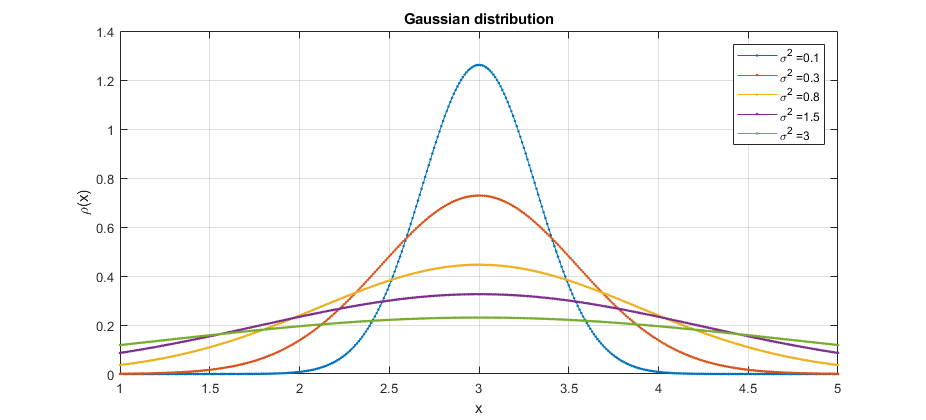
\includegraphics[width=\textwidth]{gaussian.png}
    \caption{Example of Gaussian probability density functions according to its variance.}
    \label{gaussian}
\end{figure}

\color{blue!40!black}\chapter{Forward uncertainty propagation}\color{black}
\section{Introduction}
Even if experimental tests are essential for an industrial product conception also by being a criteria for some certifications and by delivering real results to a wanted phenomena, modelling methods are getting more and more popular due to real tests important cost and by its practicality, solving physical problems relatively quickly and providing generally accurate results.
In a growing computational power context, numerical simulations applied to several domains whose mechanics and particularly CFD (Computational Fluid Dynamics), which this work will focus on, are increasing. Thus, one wants a mathematical model able to describe with best precision the true physics ; the uncertainty propagation allows one user to evaluate the model uncertainty impact on a given output from the model \cite{CoursLucor}.
In other words, how accurate is a model given a physical problem, and how its inputs may impact what is called a quantity of interest. This type of study can also provide information of an output sensibility to each parameter which it relies on.
\\\\
To study uncertainties quantification one needs to focus on the uncertain aspect of our parameters. Thus, stochastic and probabilistic methods shall be used leading to a final result that won't be just the model unique solution but a space containing all possible solutions for the given uncertain inputs. The typical uncertainty quantification and propagation loop is shown in Fig.\ref{schemalucor}.
\\\\
Let's note that uncertainty isn't what one would call error. The definition of AAIA's \cite{AIAA} for an uncertainty is a \textbf{potential} deficiency in any phrase or activity in a modelling process that is due to the \textbf{lack of knowledge}. In other hand, an error is seen as a \textbf{recognisable} deficiency that is not due to a lack of knowledge. 
\\\\
This 5 months work will focus on both forward and backward propagation of uncertainties coupled with a CFD solver. A stochastic adaptive mesh based on the stochastic error is used to provide even more accurate results especially in some high interest areas presenting singularities. %donner plus d'informations
After presenting the theoretical idea behind UQ, different techniques and some applications will be presented, including the stochastic collocation and the adaptive mesh theory.

\begin{figure}[h!]
    \centering
    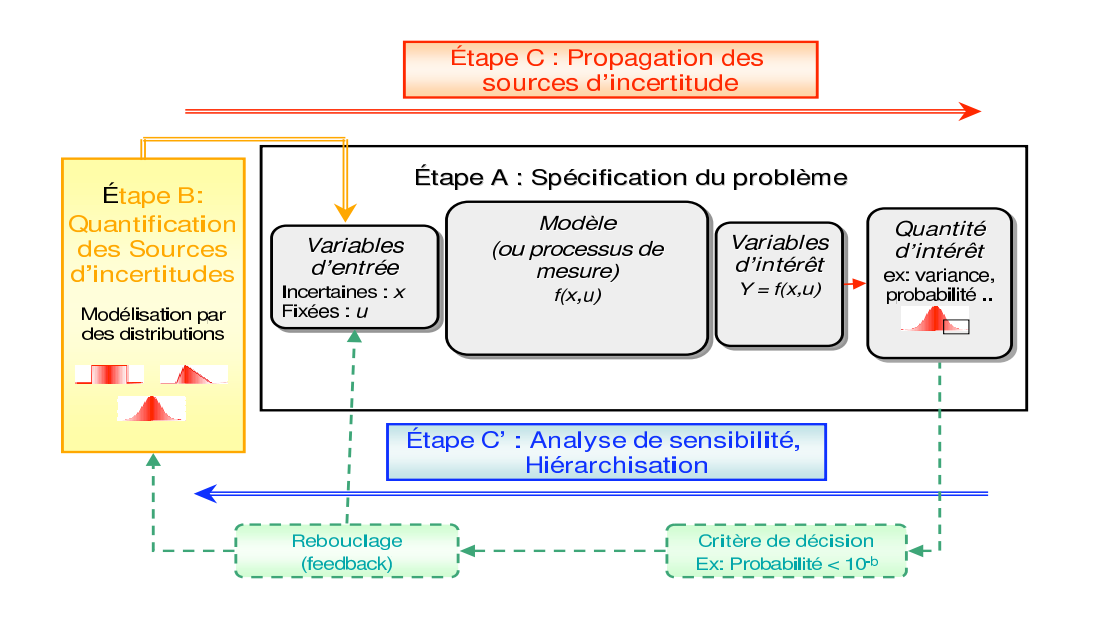
\includegraphics[width=\textwidth]{schema_lucor.png}
    \caption{Scheme of a typical framework of uncertainty quantification (à refaire)\cite{CoursLucor}}
    \label{schemalucor}
\end{figure}
Symplex elements are one of the popular geometrical elements used in CFD problems such our. A standard N symplex is made of N+1 vertices, representing nodes in computational simulation. These $\sum_{k=1}^{N+1}x_k \in \mathbb{R}^{N+1}$ nodes are linearly independents. For instance, a 0 symplex is a single point, a 2-symplex is a triangle and a 3-symplex is a tetrahedron (Fig.\ref{symplex}).
\begin{figure}[h!]
    \centering
    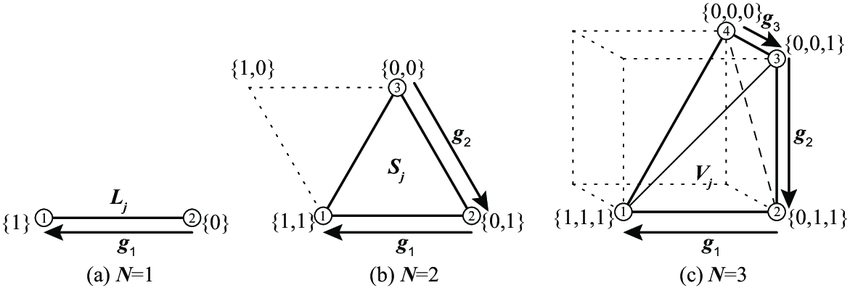
\includegraphics[width=\textwidth]{Simplex-Elements.png}
    \caption{Some symplex elements\cite{symplex}}
    \label{symplex}
\end{figure}

\section{Modelling numerical uncertainties}
Let us first introduce the various D uncertain model parameters $\boldsymbol{\xi}$ = $(\xi_1, \xi_2 ... , \xi_D)$. An uncertainty quantification goal is to evaluate the stochastic response of $y(\boldsymbol{\xi})$ (QoI) given $\boldsymbol{\xi}$. Each parameter $\xi_i$ is associated with a probability density function. Even if the full output stochastic response is wanted, it is usually unattainable. It's easier to treat the problem in a statistical way and to evaluate the output probabilistic moments.
\\\\
A robust optimisation goal is to provide the most precise solution no matter its depending constraints are i.e a accurate solution independently of the problem scenario \cite{robust}.
\subsection{Monte Carlo simulation}
A popular method for this application is the Monte Carlo simulation. This is a sampling method, in other words, with a given statistical population, one would want to study the response of our output to a random subset of individuals considering this response useful to estimate the whole population characteristics \cite{proba}. This method is robust, simple to implement and can provide very accurate results when a large number of samples is considered. Nevertheless, using Monte Carlo simulation can be very costly since the algorithm perform one deterministic computation for each sample : after calculating through a model the different $y_i$ we evaluate the $QoI = F(y_1,y_2,...,y_N)$ such as the expectation. The convergence rate follows $1/\sqrt{N}$ (not dependent on the input parameters dimension), thus, for real applications, Monte Carlo becomes quickly unaffordable in UQ studies \cite{Janthesis}. In order to reduce the computational cost of MCS, some works focused on several techniques such as the latin hypercube sampling LHS, which is a stratified MCS \cite{lhs}. Quasi Monte Carlo methods are also found (Fig.\ref{MC}), where samples are chosen in a deterministic way, improving the simulation rate of convergence. 
\subsection{Generalised polynomial chaos }
One other technique very popular in CFD applications is the generalised polynomial chaos (gPC) (chaos introduced by Wiener in 1938 \cite{gpcFirst} and gPC by Xiu and Karniadakis \cite{gpc1}, \cite{gpc2}). This method consists in approximate the QoI response by polynomials. It can be either intrusive or non intrusive ; if that case we use a Stochastic Galerkin method : the main model shall be modified, resulting in a larger system of equations to be solved (SDE). In the other hand, the non intrusive method of gPC consists on doing a pseudo spectral projection on the QoI. The original response is then approximated by a series of polynomials which leads to the closed surrogate model creation. A weakness of such method is that its convergence rate relies on how the QoI depends on $\boldsymbol{\xi}$. Since $\xi_i$ are independent, using correlated parameters proves to be difficult. Let's get into the theory mostly based on \cite{gpc1}\cite{CoursLucor}. 
\begin{figure}[h!]
    \centering
    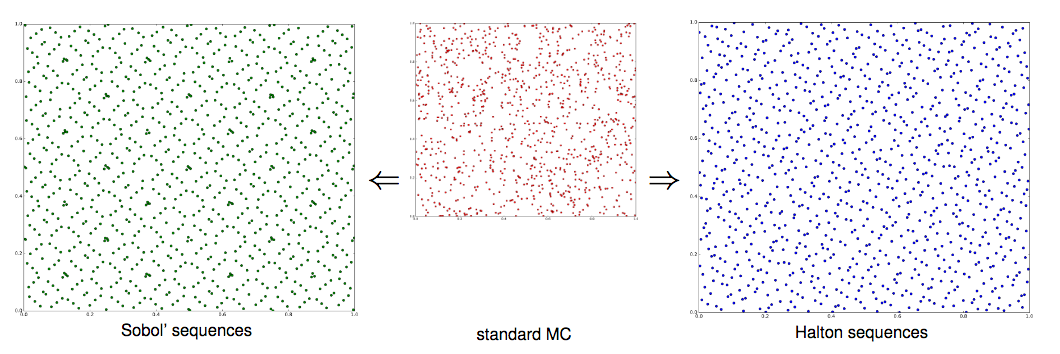
\includegraphics[width=\textwidth]{qmc.png}
    \caption{Sampling for a classic MSC and for two QMCS \cite{proba}.}
    \label{MC}
\end{figure}\\
Consider a probability space $(\Omega, \mathbb{F}, \mathbb{P})$.
The weak approximation of $y(\boldsymbol{\xi})$ is : 
$$y(\boldsymbol{\xi})=\sum_{j=0}^{\inf}u_{(j)}\Psi_{(j)}(\boldsymbol{\xi})$$
$\Psi_{(j)}(\boldsymbol{\xi}) = \prod_{i=1}^D \Psi_{i(j)}(\boldsymbol{\xi})$, with $(\boldsymbol{\xi})$ composed of independent parameters, are multivariate basis functions forming a complete basis. More over, all the basis functions are orthogonal i.e $\mathbb{E}[\Psi_i,\Psi_k]=<\Psi_i,\Psi_k>=\int_\mathbb{R}\Psi_i(\boldsymbol{x})\Psi_k(\boldsymbol{x})\rho_{\boldsymbol{x}}(\boldsymbol{x})d\boldsymbol{x} =<\Psi_i^2> \delta_{ik}$, with $\delta_{ik}$ the Kronecker delta, creating then an orthonormal basis.
$u_{(j)}$ are deterministic coefficients :
$$u_{(j)}=\frac{1}{\mathbb{E}[\Psi_j(\boldsymbol{\xi})^2]}\mathbb{E}[y(\boldsymbol{\xi}),\Psi_j(\boldsymbol{\xi})]  $$
In reality one cannot use a infinity of functions. Usually P polynomials are used in the chaos representation. The approximated quantity of interest is then :
$$y(\boldsymbol{\xi})=\sum_{j=0}^{\infty}u_{(j)}\Psi_{(j)}(\boldsymbol{\xi})+\epsilon(\boldsymbol{\xi})$$
%$\epsilon(\boldsymbol{\xi})$ 
Since the RV are now represented as a orthogonal polynomials progression, its statistical moments can be calculated through :
$$ \mu_y = \mathbb{E}[y(\boldsymbol{\xi}]=u_{(0)} $$
$$\sigma_y^2 = \mathbb{E}[(y(\boldsymbol{\xi}) - \mathbb{E}[y(\boldsymbol{\xi})])^2]=\sum_{j=1}^\infty u_{(j)}^2\mathbb{E}[\Psi_j^2(\boldsymbol{\xi})]
$$ %écrire sur les quadratures
In the case one uses the pseudo spectral approach, the model is considered as a black box. In order to calculate the $u_{(j)}$ deterministic coefficients, the deterministic solutions $y(\boldsymbol{\xi})$ are used. To do so, the expectancy $\mathbb{E}[y(\boldsymbol{\xi}),\Psi_j(\boldsymbol{\xi})]$ must be calculated :
$$\mathbb{E}[y(\boldsymbol{\xi}),\Psi_j(\boldsymbol{\xi})] = \int_{\mathbb{R}} y(\boldsymbol{\xi}) \Psi_j (\boldsymbol{\xi}) \rho_{\boldsymbol{\xi}} (\boldsymbol{\xi}) d\boldsymbol{\xi}$$
Since one cannot calculate exactly this integral, numeric quadrature is used. This method allows an integral to be estimated in a discrete way. Let's introduce a g function such as $g(\boldsymbol{\xi}) = y(\boldsymbol{\xi}) \Psi_j (\boldsymbol{\xi})$. The numerical quadrature goal is to evaluate :
$$ Q^N[g] := \mathbb{E}[g(\boldsymbol{x})]] = \int_{\Omega^N} g(\boldsymbol{\omega}) dP_{\boldsymbol{\xi}}(\boldsymbol{\omega})$$ 
where $\boldsymbol{w}$ is a N vector dimension of weights. An approximation of this quadrature is made using $N_e$ points between the quadrature points (sub-element) $\boldsymbol{Z} \in \Omega^N = \{Z^{(1)},..., Z^{(N_e)}\}$. The quadrature formula becomes then \cite{CoursLucor}:
$$Q_{N_e}^N [g]= \sum_{i=1}^{N_e} \boldsymbol{w}^{(i)} g(\boldsymbol{Z}^{(i)})$$
This approached quadrature can either be stochastic or deterministic. An example of a stochastic one is using a Monte Carlo calculus, considering all $w^{(i)}$ as $1/N_e$:
$$Q_{N_e}^N [g]= \frac{1}{N_e}\sum_{i=1}^{N_e}  g(\boldsymbol{Z}^{(i)})$$
Similarly to the MCS method, this quadrature convergence rate follows ($N_e^{-1/2}$) and doesn't relies on the dimension N. In the other hand, the Gauss quadrature uses a weight function to estimate the integral. We won't go deep into these two techniques theory since the Newton cotes quadrature is used in this work. This method is based on equidistant polynomial interpolation : a n-point NC rule uses then an n-1 degree polynomial to approximate the function. This quadrature approximation leads to a non intrusive approach. Advantages concerning this technique compared to the Gauss quadrature are that we need less quadrature points to evaluate an integral. Indeed, most NC quadrature points are located on the symplex elements boundaries which are therefore used for approximating the response in multiple elements (Fig.\ref{newtoncotes}). More over, to get a polynomial approximation or order p results for n uncertain parameters we use $(p + 1)^n$ samples per element in the Gauss quadrature where as we need $(n+p)!/(n!p!)$ samples per element. Thus a NC quadrature elements increases less rapidly when one tries to get a better approximation. For instance, a first order polynomial NC is the trapezoidal rule between two points. The second order NC quadrature uses the Simpson's rule \cite{NCquadrature}. 
\begin{figure}[h!]
    \centering
    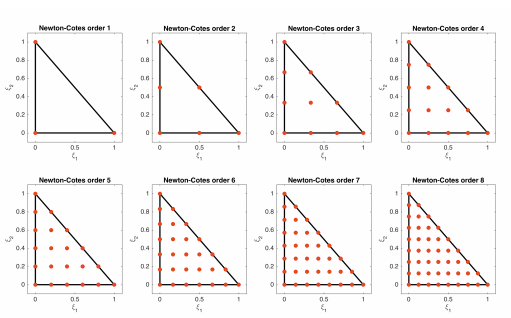
\includegraphics[width=\textwidth]{NC.PNG}
    \caption{Example of Newton Cotes quadrature points in a 2D element \cite{Janthesis}.}
    \label{newtoncotes}
\end{figure}
\\\\
PC was used by many authors in UQ associated to CFD. Hosder et al \cite{Hosder} applied a non intrusive PC in three stochastic fluid dynamics problems : an inviscid oblique shock wave problem with geometric uncertainty, an inviscid expansion wave problem with geometric uncertainty and a 2D, subsonic, laminar boundary layer flow over a flat plat with an uncertain free stream dynamic viscosity. Statistics obtained with such method were compared to MC simulations results, and a fourth order polynomial chaos expansion approached the wanted accuracy regarding the MC results (excepting for the first test case, where a sixth expansion order was required). J. -C. Chassaing and D. Lucor \cite{JC} coupled a non intrusive stochastic spectral approach with a compressible solver to propagate uncertainties around a NACA0012 airfoil. Uncertain parameters where the free stream Mach number and the angle of attack. An error analysis concerning the physical and stochastic discretization was also made and results showed that the free stream Mach number mostly drives mechanism in the aerodynamic output probability density function. This method delivered accurate representation of the solution and statistics and was computationally low cost. \cite{sto1}. Wan and Karniadakis \cite{wan&karnia} applied a Multi Element gPC on the Kraichnan–Orszag three mode problem and in advection-diffusion problems in order to deal with stochastic differential equations discontinuities. ME gPC main idea is to separate the space where a given error in variance exceeds a threshold value, and to apply a gPC expansion in each sub-domain. Results showed that contrarily to the classic gPC method, the ME gPC can capture the discontinuity by decomposing the random space. More over ME gPC has been shown as efficient regarding stochastic PDEs which contain no or small subsets of discontinuities.
\subsection{Stochastic Collocation}
The stochastic collocation, also called the probabilistic collocation method  is also a popular method to solve complex systems where a a well established model exists. It was first developed by  Mathelin and Hussaini \cite{NasaSCM}. 
This method main idea is to aim the residue of the deterministic governing equations to be zero at discreet nodes in the computational domain. These nodes are also called collocation points. Thus, in contrary of classical sampling methods, the stochastic collocation is a method that leads to strong converged results, close to the true solution. That means that if we consider $\theta_M = \{Z^{(j)}\}_{j=1}^M$ a set of given nodes in a random space (thus, our inputs in a stochastic grid) and $\{y^{(j)}\}_{j=1}^M$ the deterministic solution of a given model, we introduce $w(\boldsymbol{Z})$ which shares with Z the same polynomial space $\Pi(Z)$. $w(\boldsymbol{Z})$ is an approximation to the true solution $u(\boldsymbol{Z})$ which means that $||w(\boldsymbol{Z}) - u(\boldsymbol{Z})||$ is sufficiently small. Thus, a convergence of stochastic collocation requires that 
$$||w(\boldsymbol{Z}) - u(\boldsymbol{Z})||\longrightarrow 0$$ when $M \longrightarrow \infty$. One can find two stochastic collocation approaches : the interpolation approach and the discrete projection approach, also called the pseudo spectral approach \cite{xiu}. This work will use a Simplex Stochastic Collocation method (SSC) introduced by Witteven and Iaccarino \cite{SSC}, which relies on the Delaunay triangulation to divide a given space into simplexes over which interpolation and integration can be made. One can get a good approximation of a given QoI using SSC with less computational effort since the local refinement is based on the QoI local behavior. More over this technique was first developed to deal with with non hypercube probability spaces, making it attractive for models using probability correlated input parameters.\\\\
The interpolation approach goal is to efficiently approximate $y$ by an expansion of $w(\boldsymbol{Z})$  in Lagrange polynomials so one has :
$$ w(\boldsymbol{Z}) = \sum_{j=1}^M u(Z^{(j)}) L_j(\boldsymbol{Z}) $$
Where $ L_j(\boldsymbol{Z}) = \delta_{ij}$. Both means and variance can be then calculated using the Newton Cotes quadrature associated to stochastic nodes in the symplex element. So, the integral over the whole probability space is approximated by a summation of integrals over $N_\Omega$ sub-elements $\Omega_i $ \cite{Witteven} :
$$\mathbb{E}[w(\boldsymbol{Z}] = \sum_{i=1}^{N_\Omega}\int_{\Omega_i} w(\boldsymbol{Z})\rho_{\boldsymbol{Z}}d\boldsymbol{Z} = \sum_{i=1}^{N_\Omega}\sum_{k=1}^{Ne}c_{(i,k)}w(\boldsymbol{Z_{i,k}})$$
where $Ne$ are deterministic samples in each element (i.e quadrature points). $c_{i,k}$ are the quadrature weights which are directly linked to the parameters density functions under a sub-element :
$$c_{(i,k)}=\int_{\Omega_i} L_{(i,k)}(Z_1,...,Z_M)\rho_{\boldsymbol{Z}}(Z_1,...,Z_M)d\boldsymbol{Z}  $$
with $i=1,...,N_\Omega$. This approaches results in a polynomial chaos formulation for the given quadrature using Lagrange polynomials $L_{(i,k)}(\boldsymbol{Z})$ in the $i^{th}$ sub-element and the $k^{th}$ quadrature point. 

\color{blue!40!black}\chapter{Backward uncertainty propagation}\color{black}

Several engineering systems require today very complex models that need a large quantity of parameters. In many cases, it is difficult and sometimes impossible to get a large enough database to calibrate all parameters of a model. Often even if the experimental data is numerous a lot of samples are affected by measurements errors. Since we need a model that provides a robust solution, we need to develop efficient Uncertainty Quantification (UQ) methods, which some are presented in the last chapters. In some cases it's very difficult to evaluate directly the distribution of the model uncertain parameters. One shall then use what we call a statistical inference to approximate our parameters pdf. The inference can be followed by a forward uncertainty propagation allowing the model to get accurate predictions for quantity of interest not available before (i.e with experimental data). The next sub section focuses on some statistical inferring techniques and particularly on the Consistent Bayesian Inference presented in \cite{Tim1} and used during this 5 months work.
\section{Statistical inference}
A statistical inference is a process where a population inference (in our case, the model input uncertain parameters), are made based on statistics of a given known sample of data drawn for this population \cite{defInf}. In other words, we should be able to evaluate the probability density of our uncertain parameters $\boldsymbol{\xi}$ from a sample of known data. Two types of inferences exist : the \textbf{frequentist inference} and the \textbf{Bayesian} one. Whereas the frequentist inference focuses on the reliability of our inputs that generates their conclusions, the Bayesian is more interested in the credibility of a hypothesis given a sample of evidences \cite{statInf}. Note that both types of inferences are related to a statistical point of view that sometimes bring specialists to long discussions and disagreements.

Lets introduce the conditional probability concept, which is central to understanding both inference point of views. Given two events A and B in $\mathcal{F}$ of a probability space $(X, \mathcal{F}, \mathcal{P})$, $\mathcal{P}(A|B)$ means the probability of A given that B has occurred and can be calculated through the \textbf{Bayes' theorem} :
$$\mathcal{P}(A|B)=\frac{\mathcal{P}(B|A)\mathcal{P}(A)}{\mathcal{P}(B)}$$


\subsection{The Bayesian Inference}
\section{The Consistent Bayesian Inference}
\subsection{Defining the inverse problem}
This subsection presents a short definition of the inverse problem as well as how to obtain the Consistent Bayesian inference solution mostly based on \cite{Tim1}. \\\\
Let $(\Lambda, \mathcal{B}_\Lambda, \mu_\Lambda)$ and  $(D, \mathcal{D}_\Lambda, \mu_D)$ be two measurable spaces. Consider now a deterministic model $M(\lambda, Y)$ related to the solution $Y(\lambda)$ function of $\lambda \in \Lambda \subset \mathbb{R}^n$, $\lambda =\{\lambda_1, \lambda_2,..., \lambda_n$\}, $n \in \mathbb{N}$. In the case of uncertainty propagation and quantification, we want to study a quantity of interest which we denote by $\{Q_i(Y)\}_{i=1}^{m}$. Since $Y$ is a function of $\lambda$, we will denote the QoI by $Q_i(\lambda) : \Lambda \rightarrow D \subset \mathbb{R}^m$. Note that $D$ represents the range of the QoI map. For the definition of an inverse problem we must assume that Q defines a measurable mapping between the two previously defined measure spaces i.e Q is at least piece wise smooth in D. Thus, for any event $A \in \mathcal{B}_D$, the measurability of Q implies that 
$$ Q^{-1}(A) = \{ \lambda \in \Lambda | Q(\lambda) \in A\} \in \mathcal{B}_\Lambda $$
That implies 
$$Q(Q^{-1}(A)) = A $$
Now, let's assume that we dispose of an observed probability measure $P_D^{obs}$ on $(D, \mathcal{B}_D)$, that is absolutely continuous with respect to $\mu_D$ and thus, thanks to the Radon Nykodim theorem, admits an observed probability density $\pi_D^{obs}$. During the inverse problem process, we seek a probability measure denoted $P_\Lambda$ on $(\Lambda, B_\Lambda)$, absolutely continuous wtr $\mu_\Lambda$ so if we propagate it through the model, we obtain the observed measure for all $A \in \mathcal{B_D}$. From now on, we use $P_D^{Q(P_\Lambda)}$ to describe the push forward of a $P_\Lambda$ through $Q(\lambda)$ that satisfies :
$$ P_D^{Q(P_\lambda)}(A) = P_\Lambda (Q^{-1}(A))$$
$\forall A \in \mathcal{B_D}$
Thus, the main inverse problem goal is, given $\pi_D^{obs}$, to find the probability density $\pi_\Lambda$ such that the push forward measure induced by $Q(\lambda)$ satisfies :
$$ P_D^{Q(P_\lambda)}(A) = P_\Lambda (Q^{-1}(A)) = P_D^{obs}$$
$\forall A \in \mathcal{B_D}$. \\\\
Every probability that satisfies the equality above is called a consistent solution.
The inverse problem being defined we introduce some important terms that are used in classical inference problems to allow the reader to better understand the following procedures. To solve the inverse problem, we need to define a prior probability measure $P_\Lambda^{prior}$ on $(\Lambda, \mathcal{B}_\Lambda)$ continuous wtr $\mu_\Lambda$ related to its density $\pi_\Lambda^{prior}$. The prior measures the existing knowledge that we have at first concerning the uncertain parameters of the model. Thus, using the expression above, we have for all $A \in \mathcal{B}_D$ :
$$ P_D^{Q(prior}(A) = P_\Lambda^{prior} (Q^{-1}(A))$$
In order to present a final consistent solution to the inverse problem, the last must be solvable. Indeed, $\pi_D^{Q(prior)}$ may not exist with respect to $\mu_D$. One must then consider some assumptions.
\\\\
Assumption 1 : Either the measure $\mu_D$ is defined as the push forward volume measure, or the push forward volume measure is absolutely continuous with respect to $\mu_D$. With this assumption we have for any $A \in \mathcal{B}_D$,
$$ P_D^{Q(prior}(A) = \int_A \pi_D^{Q(prior)} d\mu_D = \int_{Q^{-1}(A)} \pi_\Lambda ^{prior} d\mu_\Lambda = P_\Lambda^{prior} (Q^{-1}(A))$$
More over, the same issue is related to the observed distribution $\pi_D^{obs}$, which must be absolutely continuous wrt $\mu_D$. Thus, we need a second assumption.\\\
Assumption 2 : There exists a constant C > 0 such that $\pi_D^{obs} \le C \pi_D^{Q(prior)}$
for almost every $q\in D$. This assumption implies that the observed measure is continuous with respect to the measure in D.
\newpage
\subsection{A consistent Bayesian solution to the stochastic inverse problem}
Authors in \cite{Tim1} show that one solution can be obtained from simple probability laws, but the solution can fail to be a probability measure on $(\Lambda, B_\Lambda)$ thus to be consistent. This problem leads to the utilization of the disintegration theorem \cite{desintegration}. From measure theory to our problem context we state this theorem below :
\\\\
\textbf{Disintegration Theorem} : \textit{Assume} $Q:\Lambda \rightarrow D$ $B_\Lambda$ \textit{measurable}, $P_\Lambda$ is a probability measure on $(\Lambda, B_\Lambda)$ and $P_D$ is the push forward measure of $P_\Lambda$ on $(D, B_D)$. There exists a $P_D$ almost everywhere uniquely defined family of conditional probability measures $P_q$, $q \in D$, on $(\Lambda, B_\Lambda)$ such that for any $A \in B_\Lambda$,
$$P_q(A) = P_q(A \cap Q^{-1}(q))$$
so $P_\Lambda$ can be written as an integral 
$$P_\Lambda(A) = \int_D P_q(A)dP_D(q) = \int_D(\int_{A\cup Q^{-1}} dP_q(\Lambda) )dP_D(q) $$
for $A \in B_\Lambda$. We use this theorem to define a posterior probability measure as an iterated integral. First, we apply it on the prior for a given event $A \in B_\Lambda$ : 
$$ P_\Lambda^{prior}(A) = \int_D (\int_{A\cap Q^{-1}}dP_q^{prior}(\lambda))dP_D^{Q(prior)}(q)$$
Bayes' theorem states that 
$$\pi(\lambda|q) = \pi(q) \frac{\pi(q|\lambda)}{\pi(q)}$$
We set $\pi(\lambda)\pi(q|\lambda) = \pi_\Lambda^{prior}$ to be a joint density. Since we use the disintegration theorem, Bayes' theorem is only applied on $\lambda \in Q^{-1}(q)$ so 
$$\pi(q) = \int_{\lambda \in Q^{-1}(q)} \pi_\Lambda^{prior}(\lambda) d\mu_{\Lambda,q}(\lambda)=\pi_D^{Q(prior)} $$
$\mu_{\Lambda, q}$ is the disintegration of the volume measure $\mu_\Lambda$. More over, since $\lambda \in Q^{-1}(q)$, we have $q=Q(\lambda)$. Thus from Bayes' we obtain :
$$\pi(\lambda|q) = \frac{\pi_\Lambda^{prior}(\lambda)}{\pi_D^{Q(prior)}(Q(\lambda)} $$
and
$$dP_q^{prior}(\lambda) = \frac{\pi_\Lambda^{prior}(\lambda)}{\pi_D^{Q(prior)} (Q(\lambda)} $$
Finally, writing 
$$dP_D(q) = \pi_D^{obs}(q) d\mu_D(q) $$
we define $P_\Lambda$ as a consistent solution to the stochastic inverse problem :
$$P_\Lambda(A) = \int_D(\int_{A\cup Q^{-1}} \pi_\Lambda^{prior}(\lambda)\frac{\pi_D^{obs}(Q(\lambda))}{\pi_D^{Q(prior)}(Q(\lambda))} d\mu_{\Lambda,q}(\lambda) )d\mu_D(q) $$
and the probability measure $P_\Lambda^{post}$ on ($\Lambda, \mathcal{B}_\Lambda$) can be defined as 
$$P_\Lambda^{post}(A) = \int_D(\int_{A\cup Q^{-1}} \pi_\Lambda^{prior}(\lambda)\frac{\pi_D^{obs}(Q(\lambda))}{\pi_D^{Q(prior)}(Q(\lambda))} d\mu_{\Lambda,q}(\lambda) )d\mu_D(q) $$
$\forall A \in \mathcal{B}_\Lambda$. To summarise all the important steps :
\begin{figure}[h!]
    \centering
    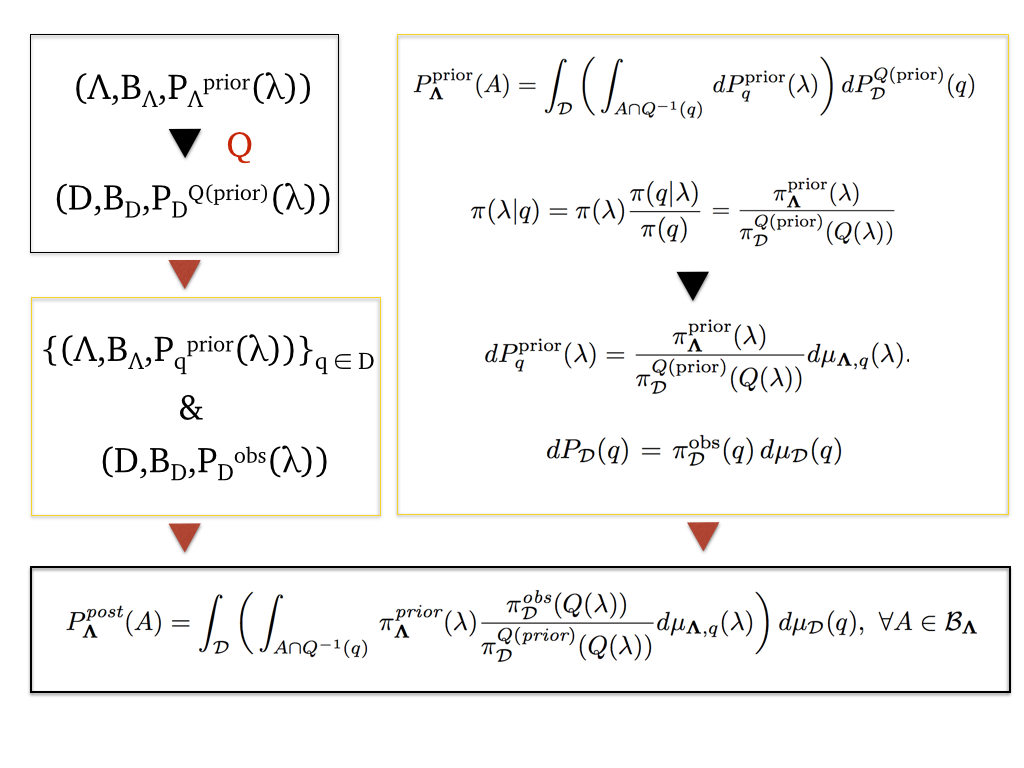
\includegraphics[scale=0.33]{schemm.png}
    \caption{The first step is the push forward of the prior. The second involves constructing the conditional probability measures from the prior measure and determining the observed density. We use then this information to construct a consistent solution in the third step.}
    \label{fig:my_label}
\end{figure}
\section{Inverse problem : Computational resolution}
For solving the numerical problem, computational considerations are made and the Consistent Bayesian Inference is used. We assume that, for test cases, $\pi_\Lambda^{prior}$ and $\pi_D^{obs}$ are given. To approximate the push forward densities $\pi_D^{Q(prior)}$ and $\pi_D^{Q(post)}$ the kernel density estimator algorithm is used (see subsection explaining how it works). The push forward propagation can be made by several techniques such as gPC, Monte Carlo inter alia. \\\\
To compute the posterior, we use samples generated from a forward propagation to estimate an approximation of $\pi_\Lambda^{post}$ :
$$\pi_\Lambda^{post}(\lambda)=\pi_\lambda^{prior}(\lambda)\frac{\pi_D^{obs}(Q(\lambda))}{\pi_D^{Q(prior)}(Q(\lambda))} $$
After the posterior computation, a rejection sampling algorithm is applied on already generated samples. This allows this method to be executed without the need of any additional deterministic calculation, which is very useful for long simulations such as CFD. The reader is invited to read the appendix for further details concerning the sampling algorithm used.
\begin{figure}[h!]
    \centering
    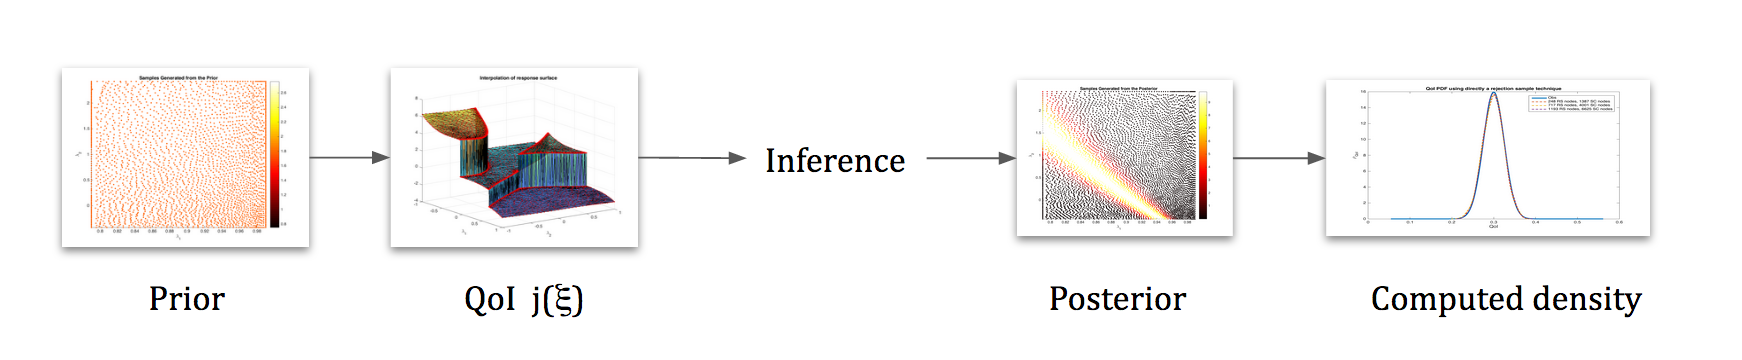
\includegraphics[width=\textwidth, height=3cm]{hec.png}
    \caption{Major steps leading to the computed QoI density}
    \label{fig:my_label}
\end{figure}
\subsubsection{Intuition}
In a computed response surface (using any type of uncertainty propagation method, such as MC, gPC or SC) we canperform the Consistent Inference. From an uniform prior (Fig.\ref{ex1rho}, (a)) we obtain a posterior distribution in $\Lambda$ (Fig.\ref{ex1rho}, (b)). The inference finds the stochastic domain where a new push forward propagation should match the observable. Those results are computed with 10000 post processing Monte Carlo samples (where the QoI is computed using the surrogate model shown in Fig.\ref{timrs1}, (a)). \\\\
From the new posterior we run a sampling algorithm (Fig.\ref{ex1pdf}, (a)) in order to compute the final QoI density which should match the observed distribution, which is here analytical ($\mathcal{N}(0.3, 0.025)$)(Fig.\ref{ex1pdf}, (b)).
\begin{figure}[htb!]

        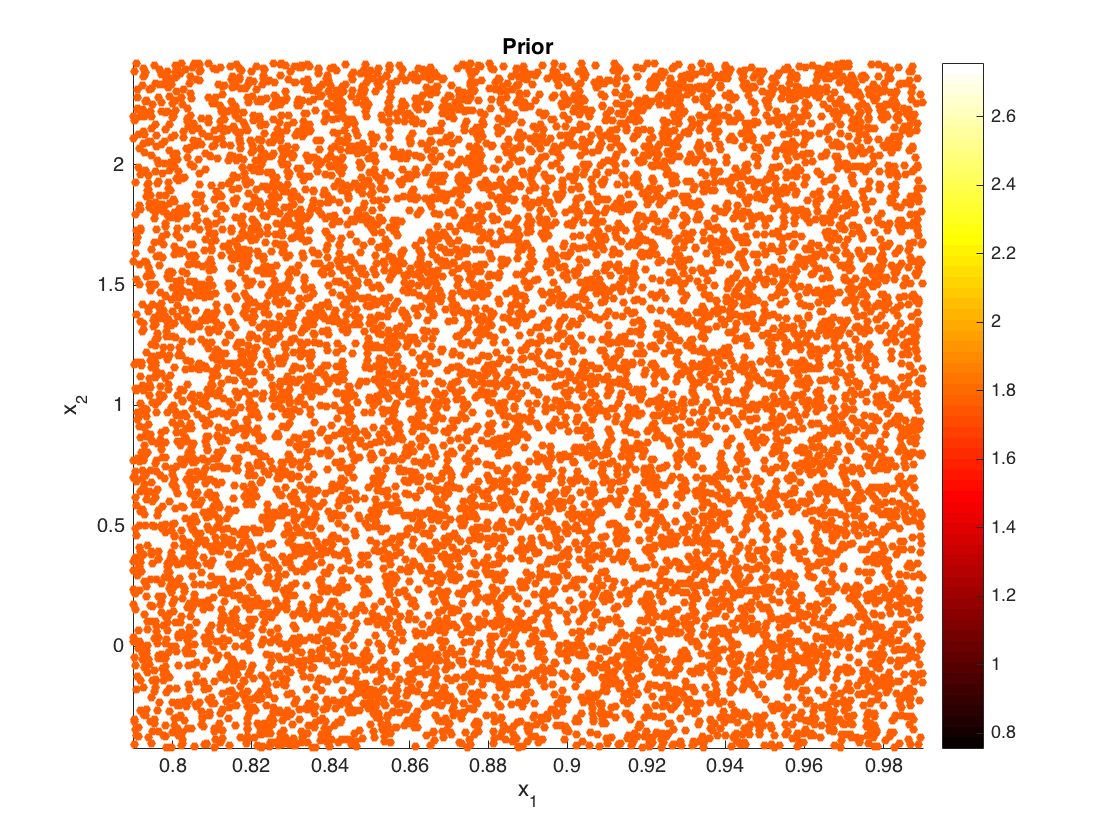
\includegraphics[width=0.49\linewidth]{ex1_prior.png}
     {\put(-220,150){\bf (a)}}
        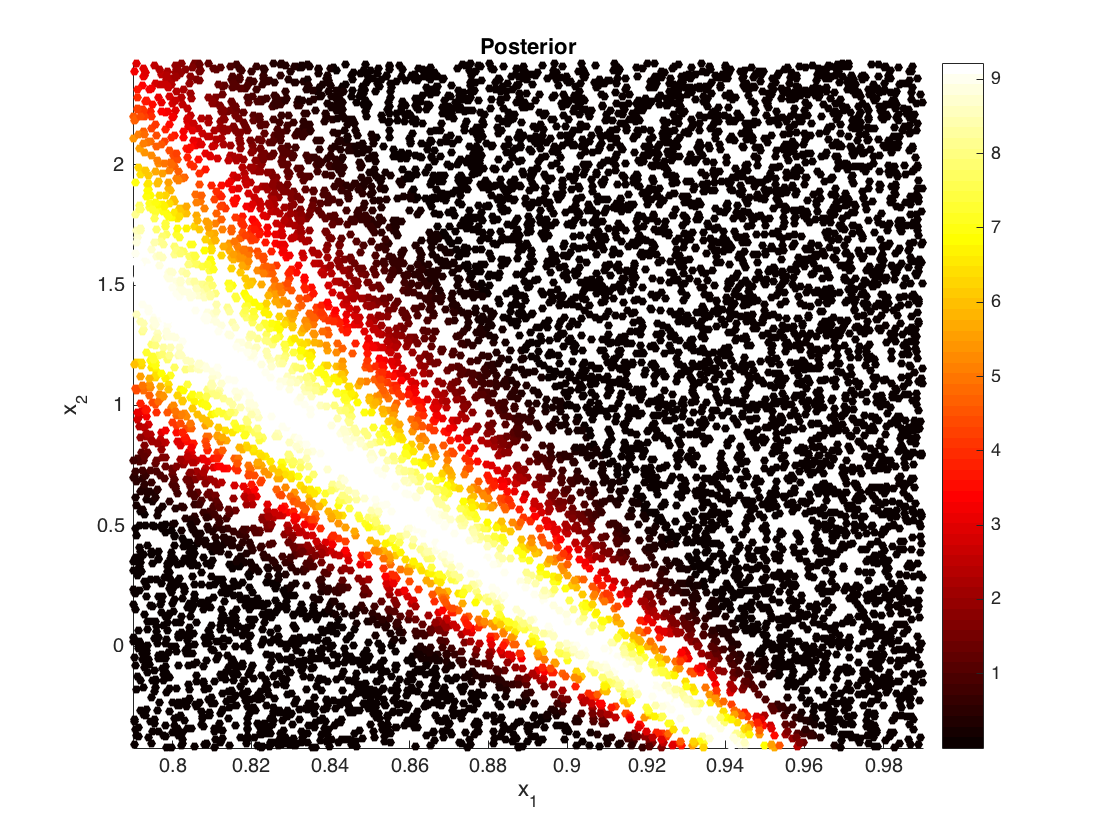
\includegraphics[width=0.49\linewidth]{ex1_post.png}
 {\put(-220,150){\bf (b)}}
    \caption{\label{ex1rho}Response surfaces for a uniform $\boldsymbol{\xi}$ distribution. (a) Stochastic simplex algorithm (b) Result from \cite{Tim1}.}
\end{figure}
\begin{figure}[htb!]

        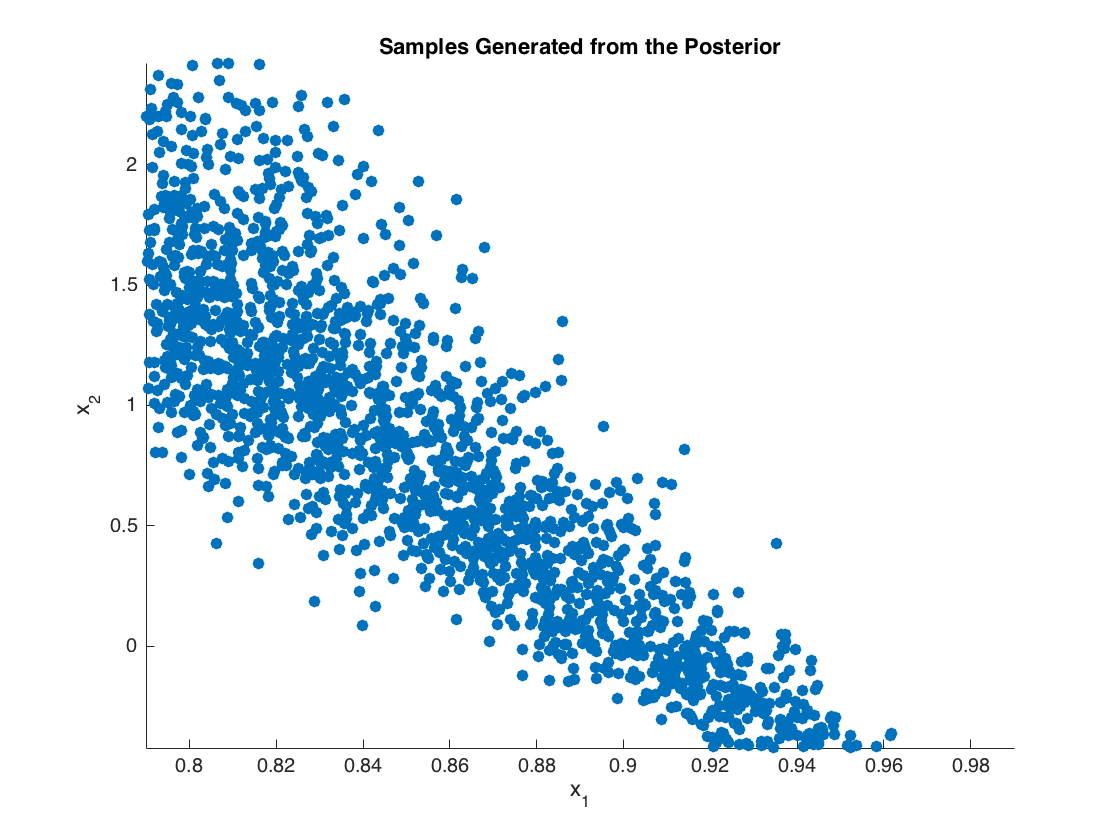
\includegraphics[width=0.49\linewidth]{ex1_RS.png}
     {\put(-220,150){\bf (a)}}
        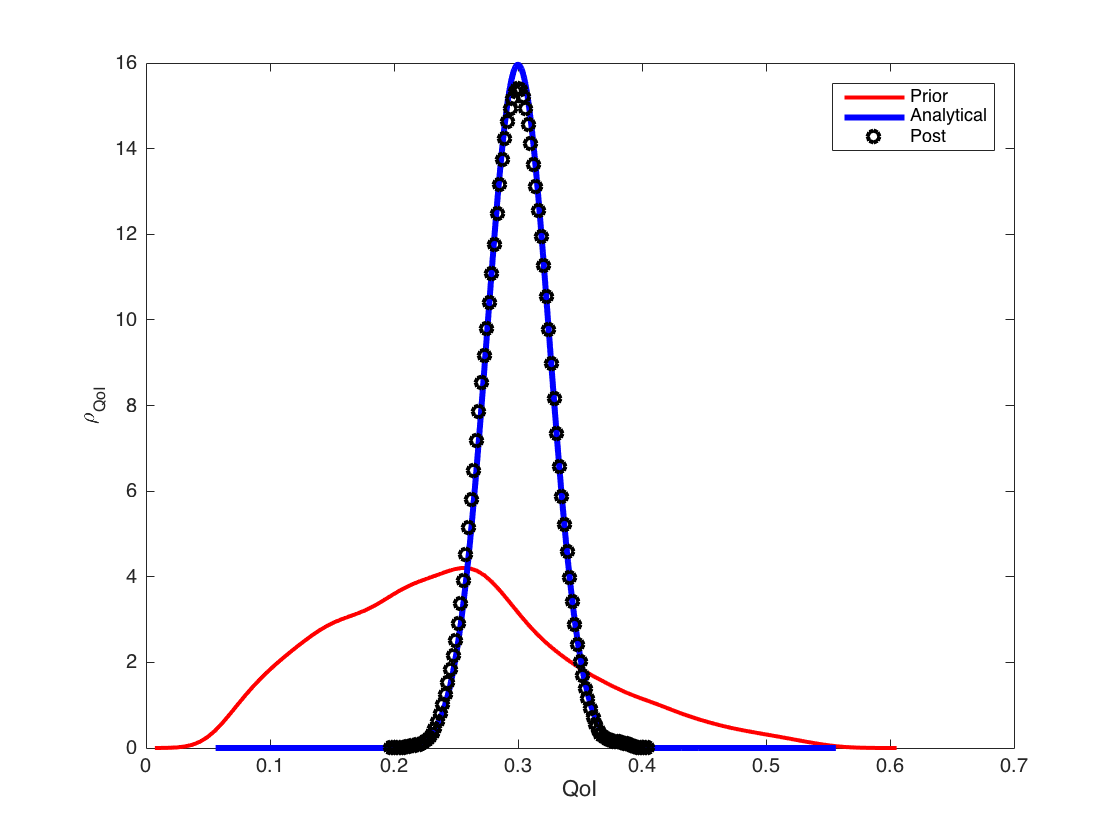
\includegraphics[width=0.49\linewidth]{ex1_pdf.png}
 {\put(-220,150){\bf (b)}}
    \caption{\label{ex1pdf}Response surfaces for a uniform $\boldsymbol{\xi}$ distribution. (a) Stochastic simplex algorithm (b) Result from \cite{Tim1}.}
\end{figure}
\color{blue!40!black}\chapter{Coupling forward and backward propagation}\color{black}
\section{Introduction}
In order to apply both type of uncertainty propagation in complex problems such as CFD models, we test the coupled method on analytical functions, mostly used by Butler et al \cite{Tim2}. We are first interested in the inverse method solution convergence. Thus, a first convergence study using crude Monte Carlo forward propagation is done. \\
The second study aims to show the efficacy of the stochastic collocation to build, with less deterministic calculation, an accurate metamodel able to detect singularities in  the QoI stochastic domain $D$. Comparisons are made with MC and gPC simulations.\\
Finally,  in order to better choose the final CFD optimisation problem, a study concerning the uniqueness of the inverse problem solution is made for several stochastic dimensions. For all problems, we use either an analytical observed distribution $\pi_D^{obs}$ or a numerically created one. 

\subsection{Analytical examples}
Analytical examples used for the following studies are presented here. To give an intuition about how the inference works, we give an example for each test case, with uniform priors. $\pi_D^{obs}$ follows, for each case :   $\mathcal{N}(0.3, 0.025)$ for the first example and $\mathcal{N}(-2, 0.25)$ for the second one, which were used in the reference paper \cite{Tim2}. 
\subsubsection{Example 1 : Non linear system}
First example is the following parameterized system for the uncertain parameters ${\xi} = [\xi_1, \xi_2]$ :
$$ \xi_1 x_1^2 + x_2^2 = 1 $$
$$ x_1^2 - \xi_2 x_2^2 = 1 $$
$x_2(\xi)$ being the functional of.  $\Lambda =$  $([0.79, 0.99],[1-4.5\sqrt{0.1}, 1+4.5\sqrt{0.1}])$. The non linear system is solved through an optimisation problem where  $\boldsymbol{x}$ is found so both expressions presented before are respected (given a chosen residual achievement goal and an initial solution), summarised by the following algorithm, for $\xi_i$, $i=1...N, N \in \mathcal{N}$.\\

\hrule 
\vspace{0.25cm}
\textbf{Algorithm : Non linear system resolution and QoI estimation}
\vspace{0.25cm}
\hrule
\vspace{0.25cm}
\textbf{for} k = 1 to $N$ \textbf{do} \\
Initialise the first couple $(x_1, x_2)_{0,k}$. \\
Evaluate the first residual $R_{0,k}$ and $J_{0,k}$. \\
\textbf{while} $|R_{iter,k}|>1e10$ and given a maximum number of iterations $iter$ \textbf{do} \\
Update $x$ values given $J_{iter-1, k}$.\\
Evaluate the new residual $R_{iter,k} $ and $J_{iter,k}$. \\
\textbf{end while}\\
\textbf{end for} \\
Choose which QoI is returned. \\
\hrule
\vspace{0.25cm}
Given $x = (x_1, x_2)_{iter}$ of an iteration, residuals and gradients are calculated through :
$$R_{iter, k} =
\begin{pmatrix}
1 \\
1
\end{pmatrix}
-
\begin{pmatrix}
\xi_1^k x_1^2 + x_2^2 \\
x_1^2 - \xi_2^k x_2^2
\end{pmatrix}
$$
$$J_{iter, k} = \Vec{\bigtriangledown} \begin{pmatrix}
\xi_1^k x_1^2 + x_2^2 \\
 x_1^2 - \xi_2^k x_2^2 = 1
\end{pmatrix} 
=
\begin{pmatrix}
2\xi_1^k x_1 + 2x_2 \\
2x_1 - 2\xi_2^k x_2
\end{pmatrix}
$$
Then $\boldsymbol{x}$ is updated :
$$ x = x + dx $$
with
$$ dx =\frac{J_{iter-1,k}}{R_{iter-1,k}} $$
The response surface computed with the stochastic collocation method is similar to the one obtained from Breit et al \cite{Tim1} (Fig.\ref{timrs1}). 
\begin{figure}[htb!]

        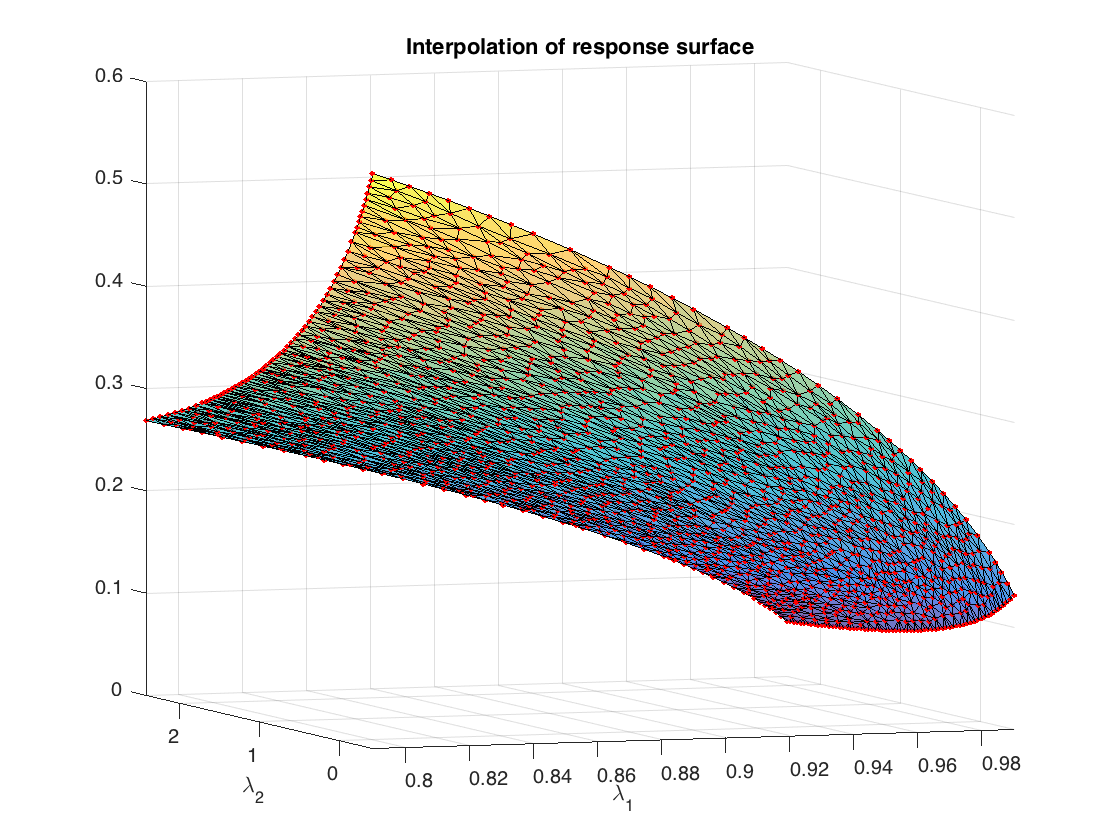
\includegraphics[width=0.49\linewidth]{Us_tim_uni_x2_rs.png}
     {\put(-220,150){\bf (a)}}
        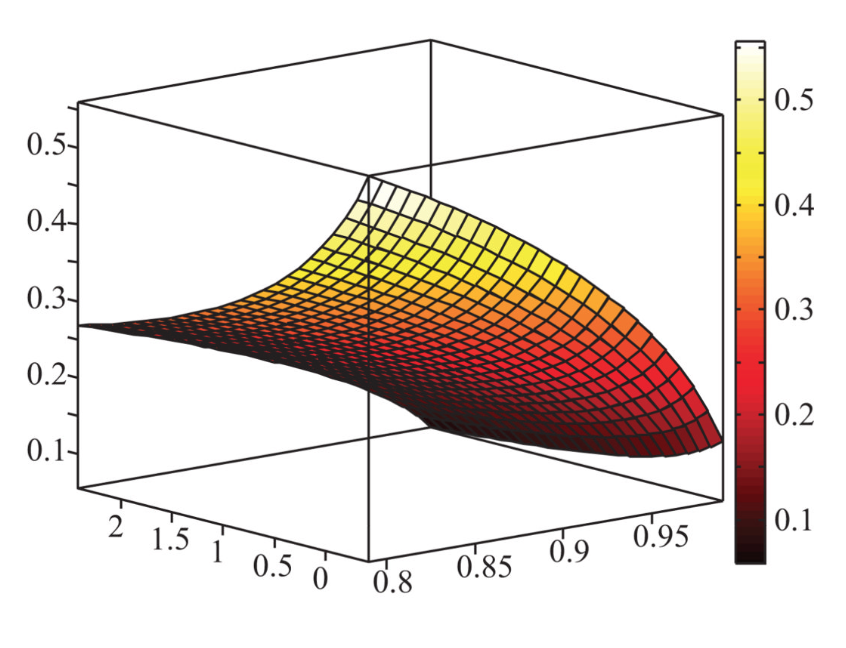
\includegraphics[width=0.49\linewidth]{Tim_response_suface_system.png}
 {\put(-220,150){\bf (b)}}
    \caption{\label{timrs1}Response surfaces for a uniform $\boldsymbol{\xi}$ distribution. (a) Stochastic simplex algorithm (b) Reference result \cite{Tim1}.}
\end{figure}\\

\subsubsection{Example 2 : Discontinuous surface}
Example 2 is a discontinuous response surface where the QoI $q(\xi)$ given ${\xi}=x_1, x_2, ..., x_d$, $d\in {N}$ is :
$$q({\xi}) = \left \{
\begin{array}{ll}
     q_1({\xi})-2 \hspace{0.1cm} \mbox{.if} \hspace{0.2cm} 3x_1+2x_2 \geq 0 \mbox{ and } -x_1+0.3x_2<0  \\
     2q_2({\xi}). \hspace{0.5cm} \mbox{if} \hspace{0.2cm} 3x_1+2x_2 \geq 0 \mbox{ and } -x_1+0.3x_2\geq 0  \\
     q_1({\xi})+4. \hspace{0.13cm} \mbox{if} \hspace{0.2cm} (x_1+1)^2+(x_2+1)^2<0.95^2 \mbox{ and } d=2 \\
     q_1({\xi}) \hspace{2.6cm} \mbox{otherwise}
\end{array}
\right.
$$
with 
$$ q_1({\xi}) = exp(-\sum_{i=1}^d x_i^2) - x_1^3 - x_2^3 ; \hspace{0.1cm} q_2({\xi}) = 1 + q_1({x}) + \frac{1}{4d}\sum_{i=1}^d x_i^2 $$
We fix d=2 and $\Lambda = ([-1,1]^2)$. The prior distribution for inferring stay uniform. Similarly to the first example, the surrogate model built approaches the one presented in the reference paper. This example if of great interest since it contains many singularities in the QoI map.
\begin{figure}[htb!]

        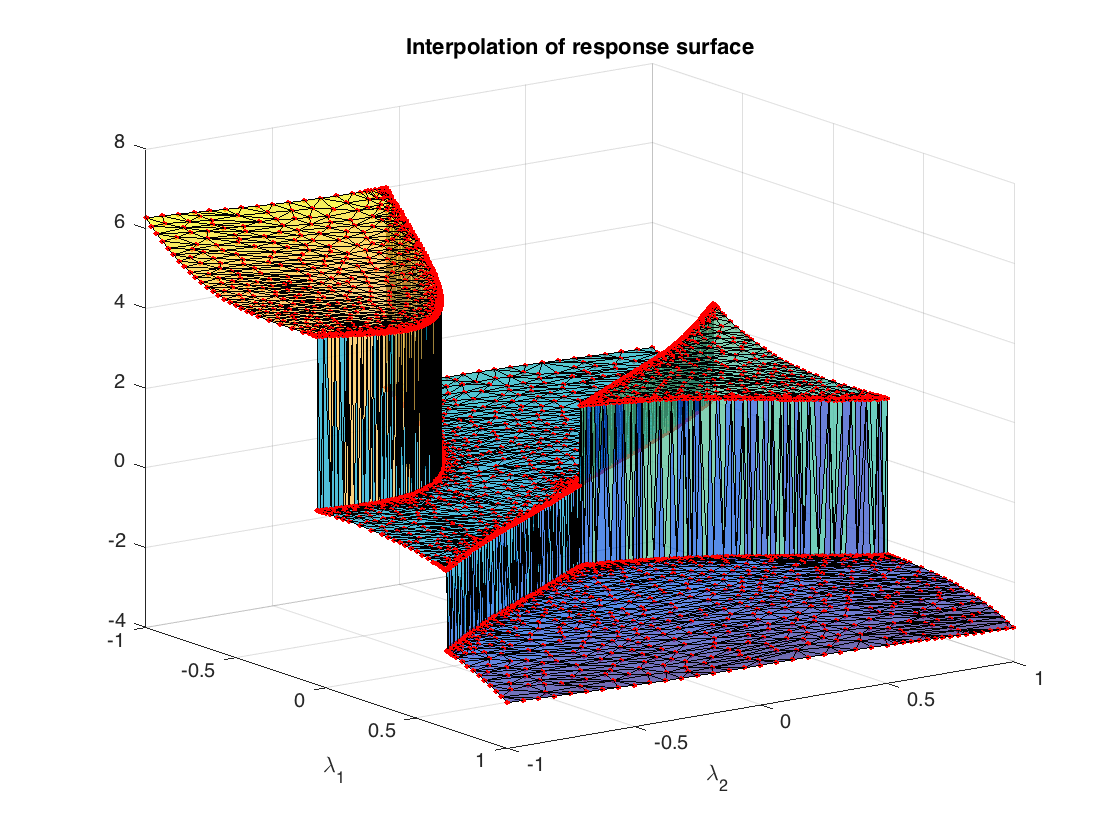
\includegraphics[width=0.49\linewidth]{Tim2_uni_rs.png}
     {\put(-220,150){\bf (a)}}
        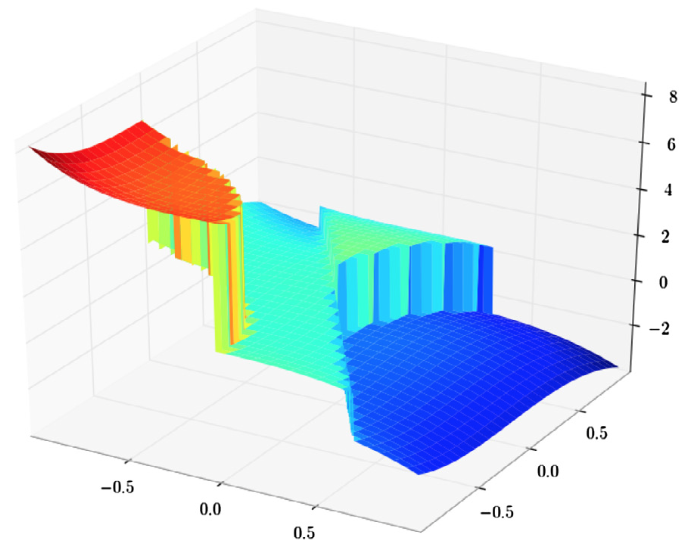
\includegraphics[width=0.49\linewidth]{castest4_paper.png}
 {\put(-220,150){\bf (b)}}
    \caption{\label{ex2pdf}Response surfaces for a uniform $\boldsymbol{\xi}$ distribution. (a) Stochastic simplex algorithm (b) Result from \cite{Tim1}.}
\end{figure}
\subsubsection{Example 3 : G-function}
We also introduce a second interest quantity computed from the G function. Uncertain parameters are  defined in $\Lambda = [0,1]^2$ : 
$$ G(x) = \prod_{i=1}^d \frac{|4x_i+2|+a_i}{1+a_i} $$
where, $\forall i = 1,..,d$ ,
$$a_i = \frac{i - 1}{2} $$
We create an observable from a independent Gaussian bi variate distribution in the $\Lambda$ space with $\mu = [0.2, 0.7]$ and $\sigma = [0.05, 0.5]$.
\section{Inference's Convergence study}
In this first study the convergence of the inverse resolution is evaluated. 

\subsubsection{Methodology}
We apply the Consistent Inference using Monte Carlo samples to push forward uncertainties. We compute then both mean and variance (and their L2 error norm) of samples from the posterior, for both analytical examples (Fig \ref{MC11}). More over, we compute the L2 norm 
$$err_{L2} = \sqrt{(m-\bar{m})^2} $$ 
between the numerical $\bar{m}$ and analytical moments that are plotted in a log log scale (Fig.\ref{MC1}, bottom). First and second statistical moments are computed with the Matlab mean and var functions, since we use Monte Carlo to the first propagation.
\subsubsection{Results}
One can see that for both examples moments converge to the expected observed values. For both examples the L2 error decreases as well as the number of samples raises.
From these results we validate the inverse method convergence. Nevertheless, where as the variance value convergence near $10^4$ samples, at least $10^5$ samples are required to get a converged QoI expectation. Also, we note that results presented in the reference paper \cite{Tim2} weren't numerically converged.\\\\ 
\begin{table}[h!]
\centering
\begin{tabular}{l|l|l|l}
\hline
Test               & sample size & $\mu$  & $\sigma^2$ \\ \hline
\multirow{2}{*}{1} & 1e4         & 0.2995 & 0.0006455  \\
                   & 1e5         & 0.2998 & 0.0006318  \\ \hline
\multirow{2}{*}{2} & 1e4         & -1.994 & 0.06628    \\
                   & 1e5         & -2.001 & 0.06554  
                   
\end{tabular}
\label{refere}
\caption{Reference values}
\end{table}
\begin{figure}[htb!]
    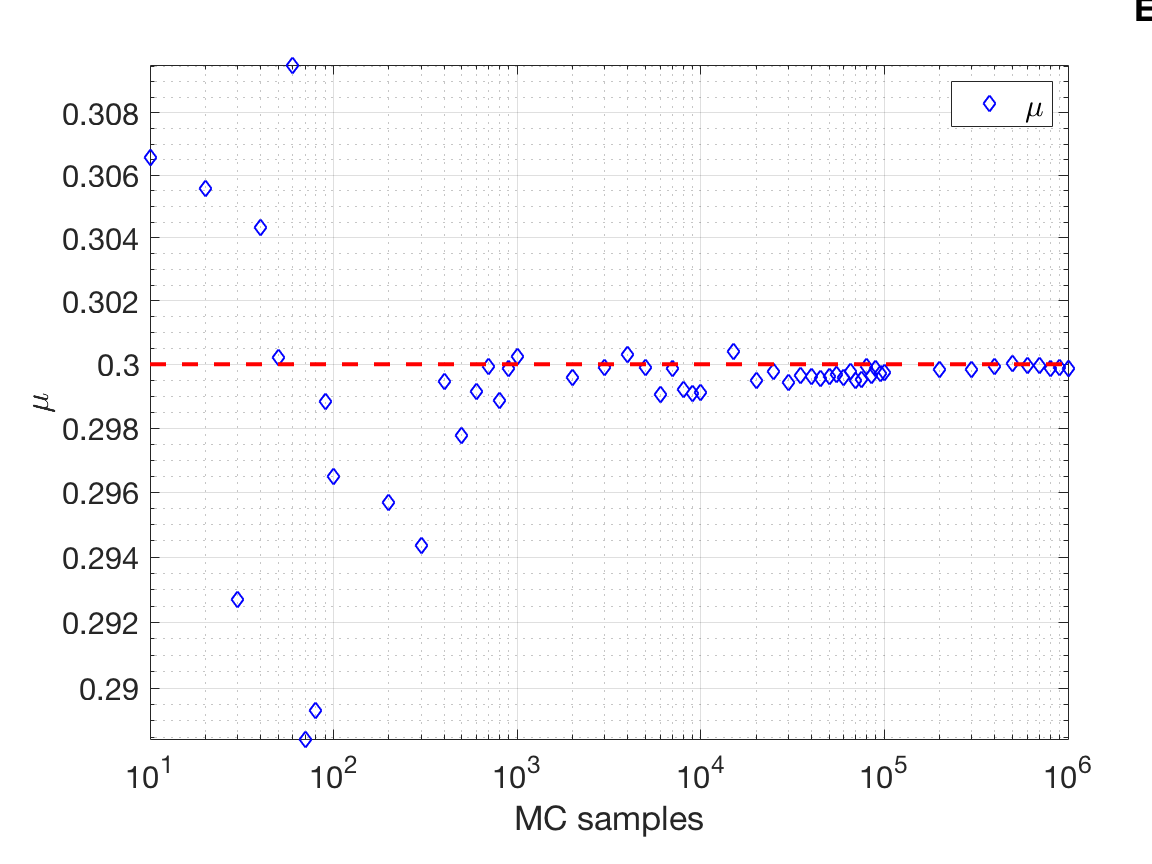
\includegraphics[width=0.49\linewidth]{ex1_1}
    {\put(-215,170){\bf (a)}}    
    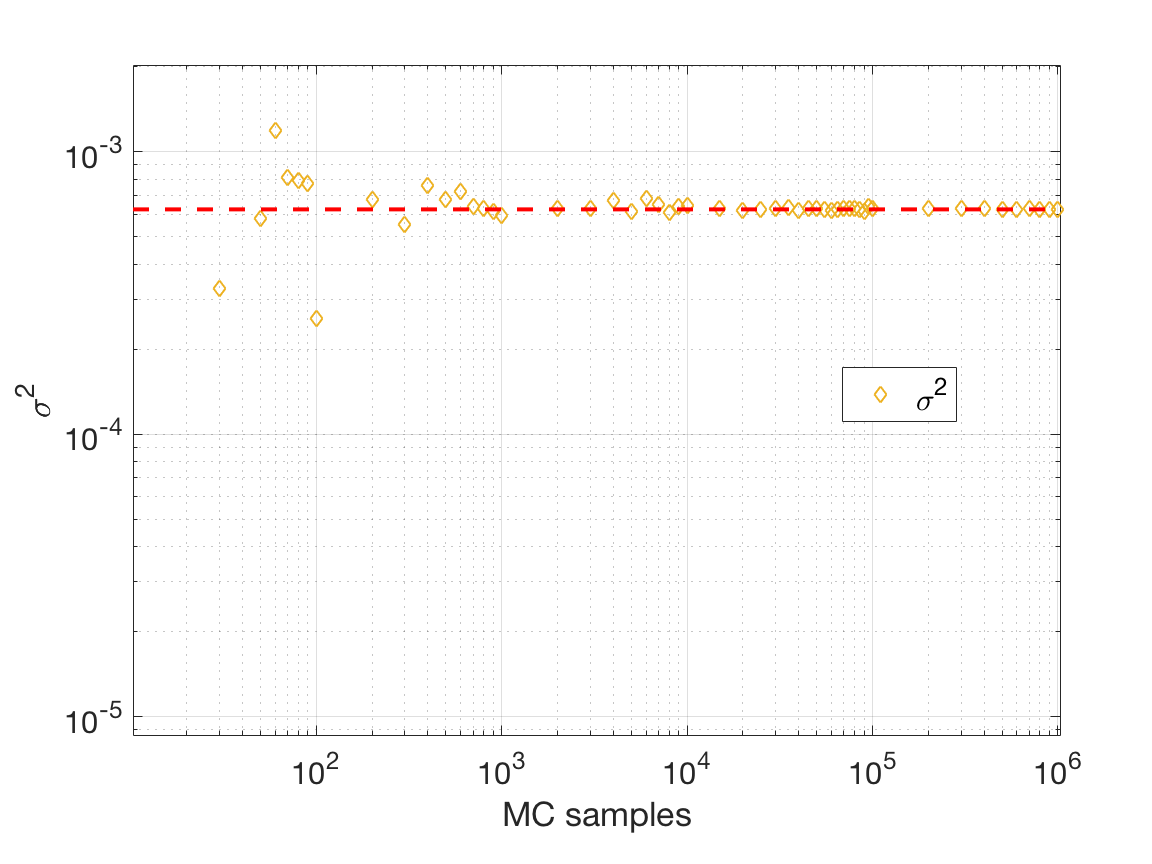
\includegraphics[width=0.49\linewidth]{ex1_2}
    {\put(-215,170){\bf (b)}}
    \caption{\label{MCex11}\textit{Convergence study results for example 1. (a) QoI Expectation following the number of MC samples (b) QoI Variance following the number of MC samples}}

\end{figure}
\begin{figure}[htb!]
    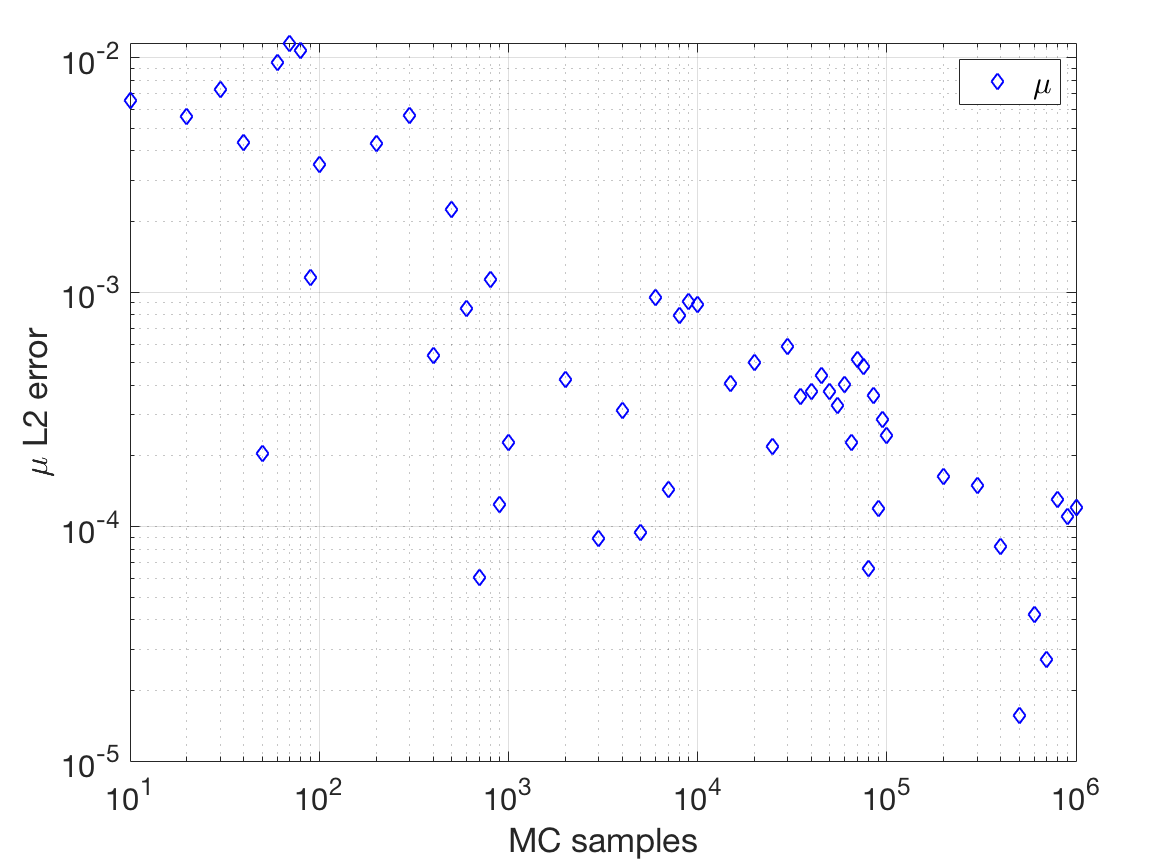
\includegraphics[width=0.49\linewidth]{ex1_3}
    {\put(-215,170){\bf (a)}}    
    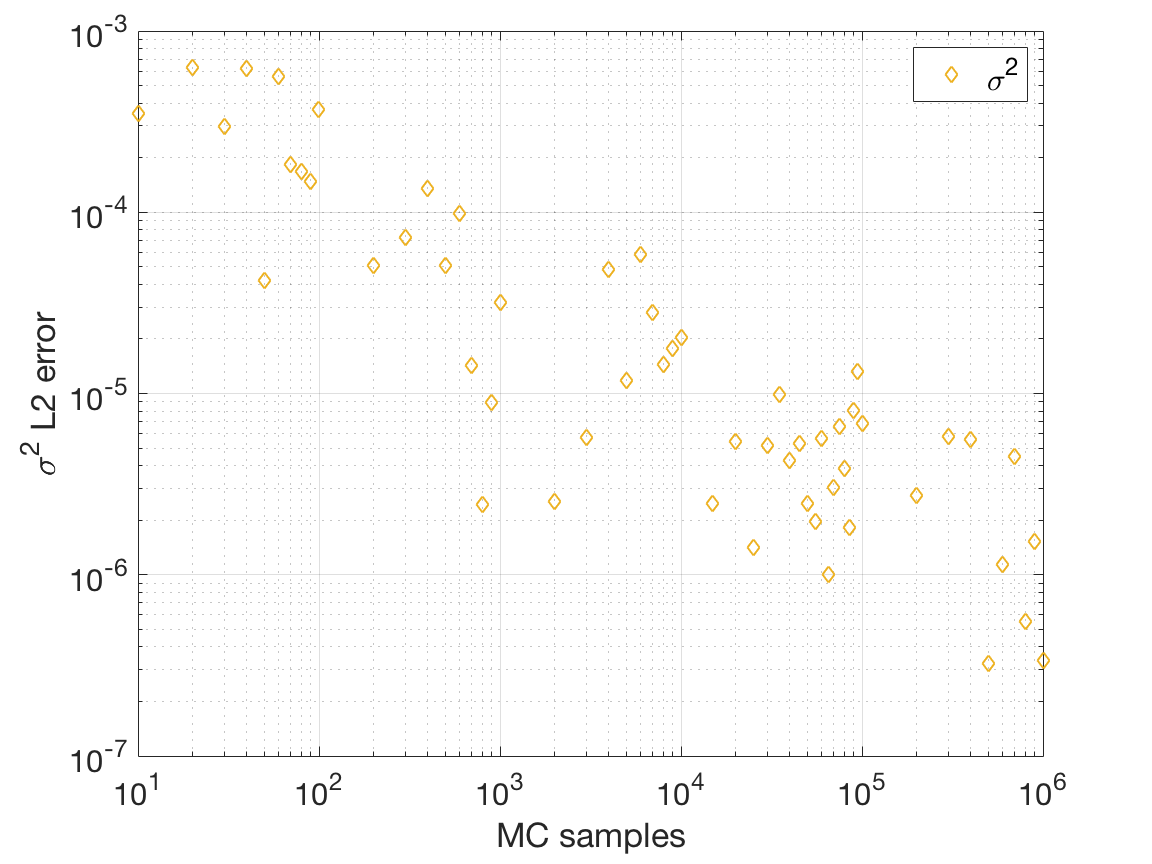
\includegraphics[width=0.49\linewidth]{ex1_4}
    {\put(-215,170){\bf (b)}}
    \caption{\label{MCex11}\textit{Convergence study results for example 1. (a) QoI Expectation error L2 norm following the number of MC samples (b) QoI Variance error L2 norm following the number of MC samples}}

\end{figure}

%%% FAIRE POUR LEX 2
\section{Metamodels comparison for the consistent inference}
One wants to evaluate, for the two presented examples which forward propagation method is the more accurate and computationally affordable. Indeed,  where as 1e6 samples can be afforded for an analytical simple problem, more complex models such as in a CFD problem can be very expensive and last long. Thus, crew MC, Lunar Hypercube Sampling (LHS), gPC and Stochastic Collocation (SC) (presented in chapter 2) and Artificial Neural Networks will be evaluated. \\\\
In a first step, we compare MC (expensive, but useful for comparison) gPC and SC results ; indeed, since we aim to apply the forward backward propagation tool to CFD, Neural Networks techniques aren't yet accurate enough. Nevertheless, its potential is still interesting to study.
\subsection{Example 1}
\subsubsection{Methodology}
We compare results from crude MC samples to the ones obtained using gPC and the Stochastic Collocation method. To do so, we evaluate moments for both methods and their errors to an observed density $\mathcal{N}(0.3, 0.025)$ and compare them to the 2 reference values (see 6.2). For the Generalized Polynomial Chaos, we apply a spectral projection method to compute the QoI of LHS samples. The Gauss Legendre quadrature and Legendre polynomials are used. We choose 5 as polynomial degree but are conscious that it could be even higher. SC moments are evaluated through post LHS samples applied on the metamodel. We compare also the L2 norm of both expectation and variance errors related to the analytical observed distribution moments. \\\\
Since for the gPC technique P=5, we use a 6x6 quadrature, thus 36 points. To make results comparable, the Stochastic Collocation metamodel is built with 36 collocation nodes. A parametric study of the number of LHS samples is carried out from 1e3 to 2e5 samples. In addition, a study comparing crude Monte Carlo moments and post processing Monte Carlo samples on a stochastic collocation is made.
\subsubsection{Results}
\begin{figure}[h!]
    \centering
    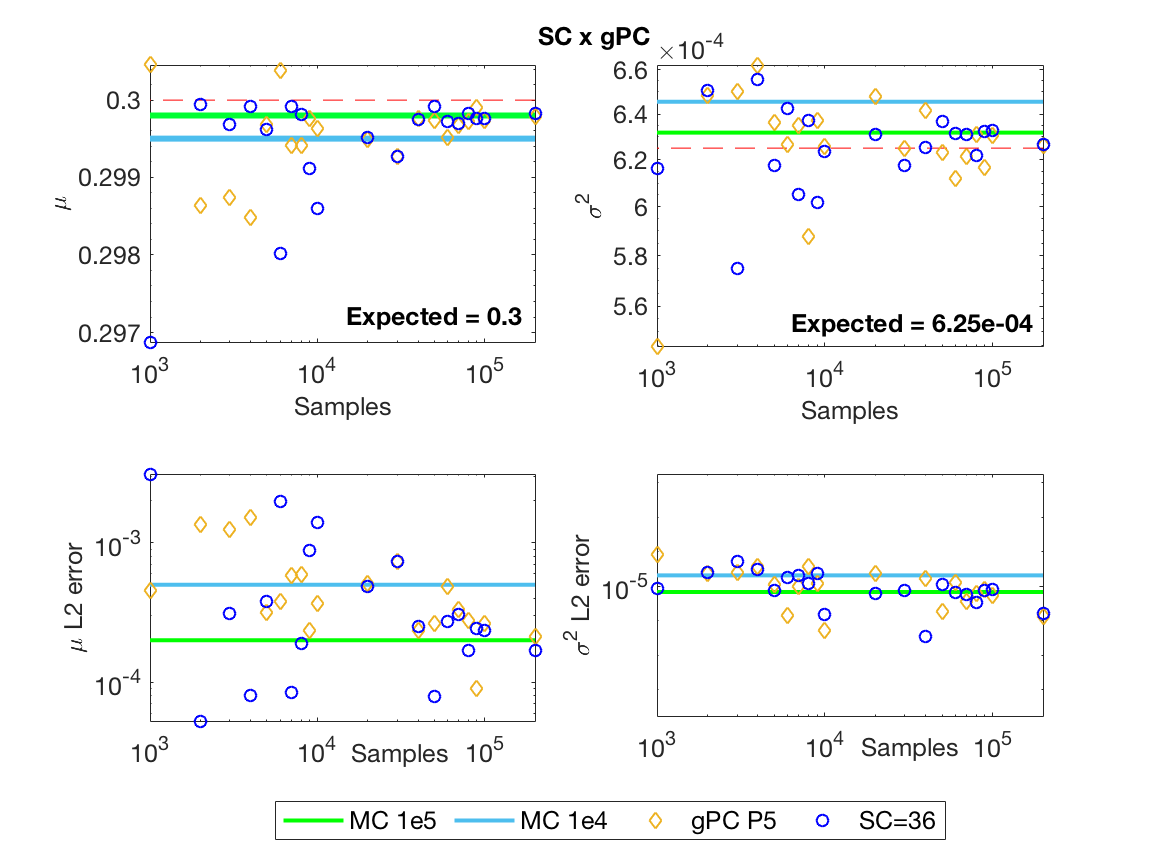
\includegraphics[width=\linewidth]{SCxGPC_moments2.png}
    \caption{SC and gPC moments compared to MC moments. Top figures : (left) Expectation, (right) Variance. Bottom figures : (left) Expectation L2 error norm, (right) Variance L2 error norm. Continuous representations are the reference MC values. x-axis are the number of LHS samples in the stochastic domain.}
    \label{comparaison1}
\end{figure}
Firstable, the moments values for both gPC and SC methods convergence while the number of LHS samples increases which is logical. Both methods seems to approaches well the metalmodel and the consistent inference works also well. Indeed, for both methods the 1e4 reference error value is underpassed before 1e4 LHS samples. The same behaviour for the 1e5 reference value. Thus, with 36 deterministic calculations, we manage to approach better the observed distribution using gPC P5 and the Stochastic Collocation. A reason for such results is a good polynomial approximation of the metamodel : for the gPC, the use of a quadrature and for the Stochastic Collocation, an adaptive mesh. \\ More over, for the same number of deterministic points, the Stochastic Collocation is better than the gPC for expectation results. Finally the error is globally very low and results seem accurate. 
%
\begin{figure}[htb!]
    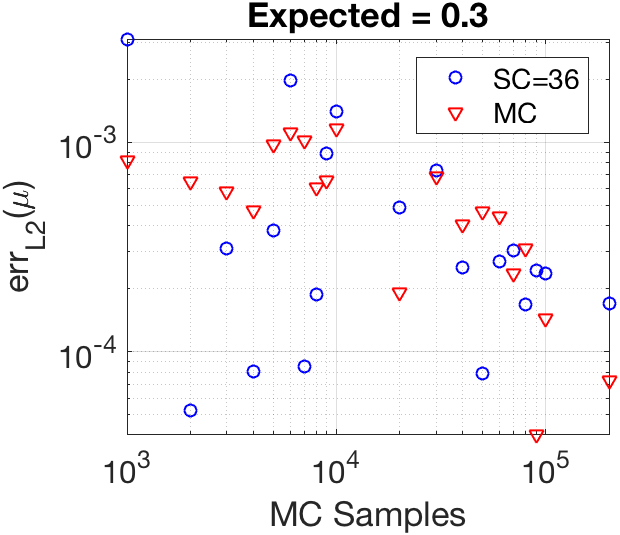
\includegraphics[width=0.49\linewidth]{muu}
    {\put(-215,170){\bf (a)}}    
    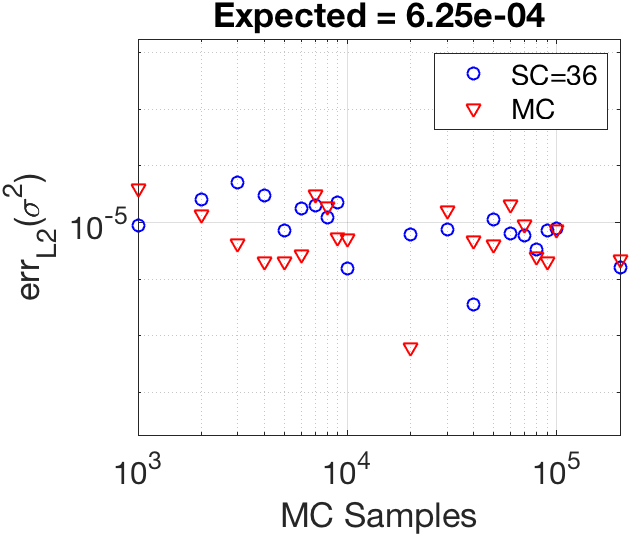
\includegraphics[width=0.49\linewidth]{sigma}
    {\put(-215,170){\bf (b)}}
    \caption{\label{SCMC}\textit{L2 error norm of two first statistical moments calculated after the rejection sampling algorithm (a) L2 norm of the expectation error for different MC sampling sizes (b) L2 norm of the variance error for different MC sampling sizes.}}

\end{figure}\\
SC results are as accurate as MC ones, while it needs way less computations. For instance, the SC method, with 36 deterministic computations has less error for both moments with $4e10^4$ post processing MC samples, compared to crud MC computations, which divides the number of deterministic computations by $10^3$.
For the second example, where discontinuities exist, we expect to observe different accuracy results.
\subsection{Example 2}
\subsubsection{Methodology}
For example 2, we want to evaluate the capacity of both methods to work with discontinuous response surfaces and provide accurate inferences regarding an observed distribution. Thus, we cannot use anymore the analytical observed distribution used by Butler et al, since the posterior was defined in a smooth sub-domain of the QoI map.
We define then a 2D distribution $\pi_\Lambda^{obs}$ in the uncertain parameters stochastic domain where, after forward propagation, leads to the QoI observable density $\pi_D^{obs}$ which is used for the consistent inference (Fig.\ref{priorobs}, right).  $\pi_\Lambda^{obs}$ follows a Gaussian distribution, with 2 uncorrelated parameters with $\mu = [0.2, 0.7]$, $\sigma_1 = 0.03$ and $\sigma_2 = 0.005$ (Fig.\ref{priorobs}, left). For both gPC and SC, we generate 1e5 LHS samples (following an uniform prior) to compute the posterior QoI distribution. 
\begin{figure}[htb!]
%
    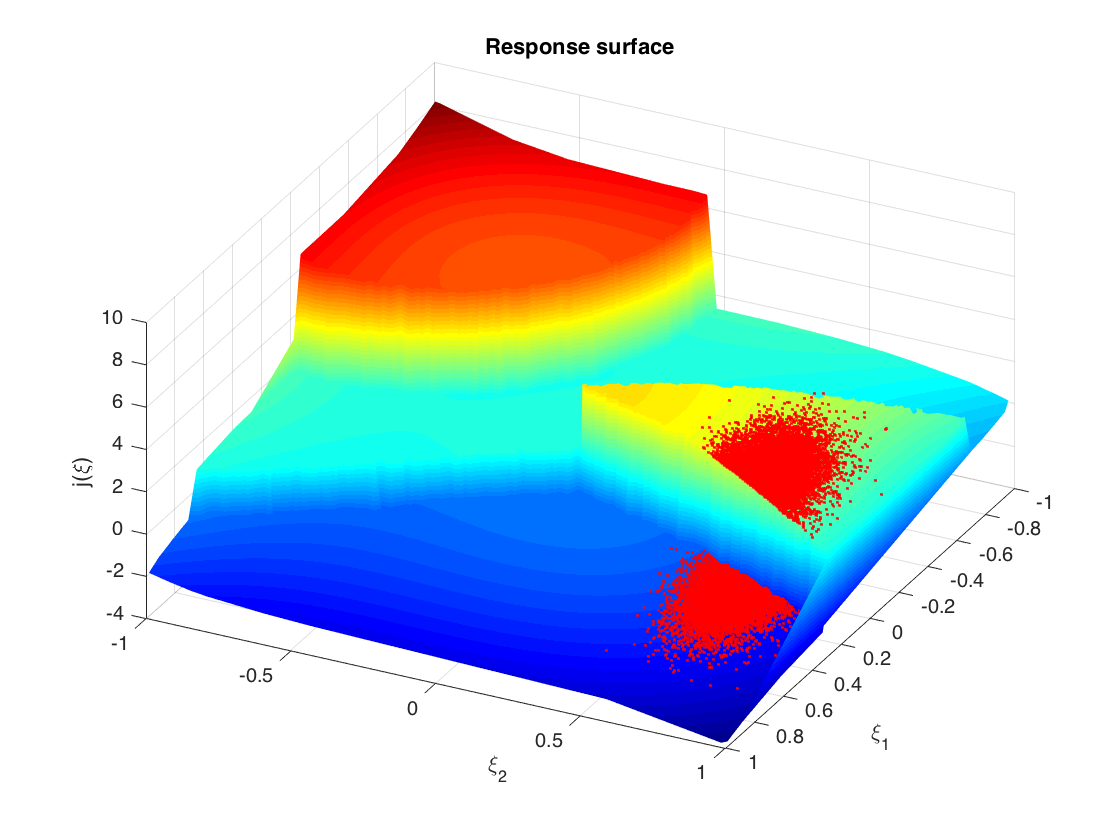
\includegraphics[width=0.49\linewidth]{priorobs.png}
    {\put(-215,150){\bf (a)}}    
    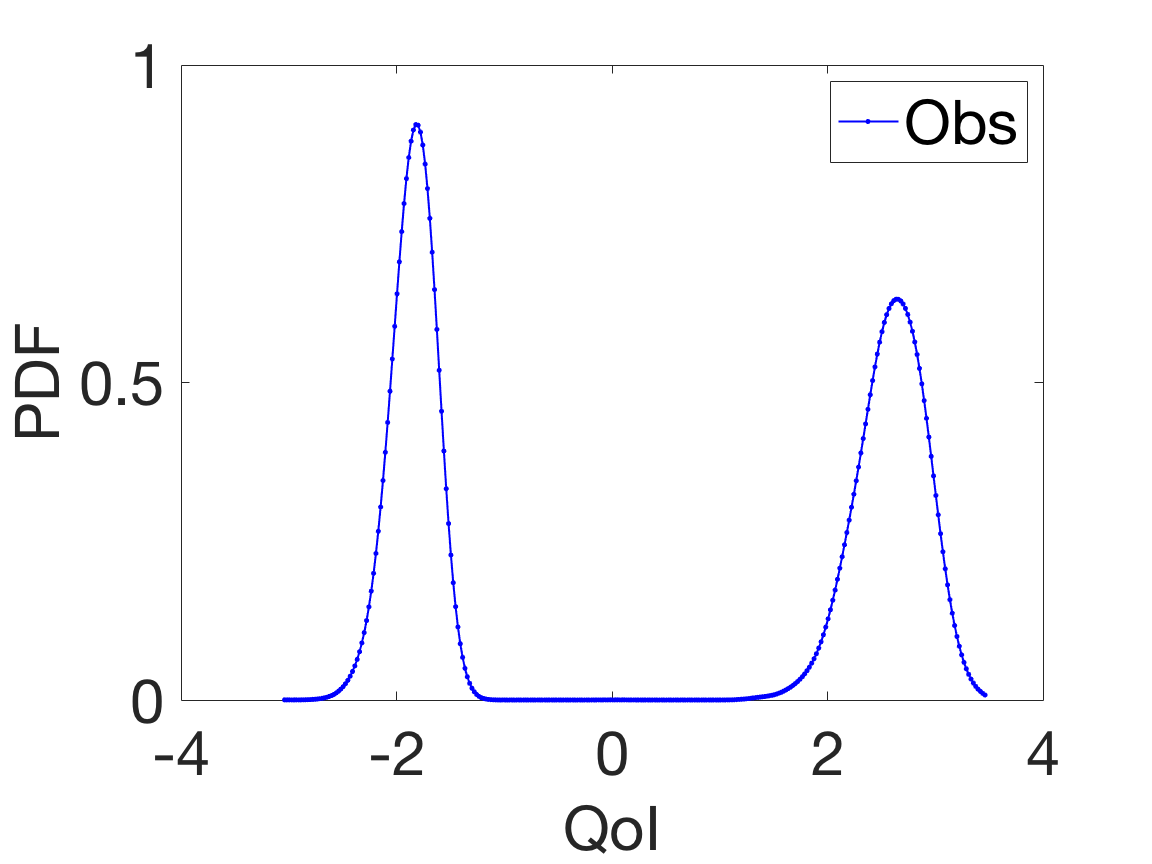
\includegraphics[width=0.49\linewidth]{Obs_default.png}
    {\put(-215,150){\bf (b)}}
    \caption{\label{priorobs} Observed distributions in both $\Lambda$ and $D$ spaces. (a) Samples generated from $\pi_\Lambda^{obs}$ on the total response surface (b) $\pi_D^{obs}$ generated with the kernel density estimation using a default bandwidth}

\end{figure}\\
Since the QoI observable is bimodal, it is hard to evaluate the different methods accuracy. Thus, a simple graphical comparison will be made between the final distributions and the observed QoI density.
\subsubsection{Results}
\begin{figure}[htb!]
%
    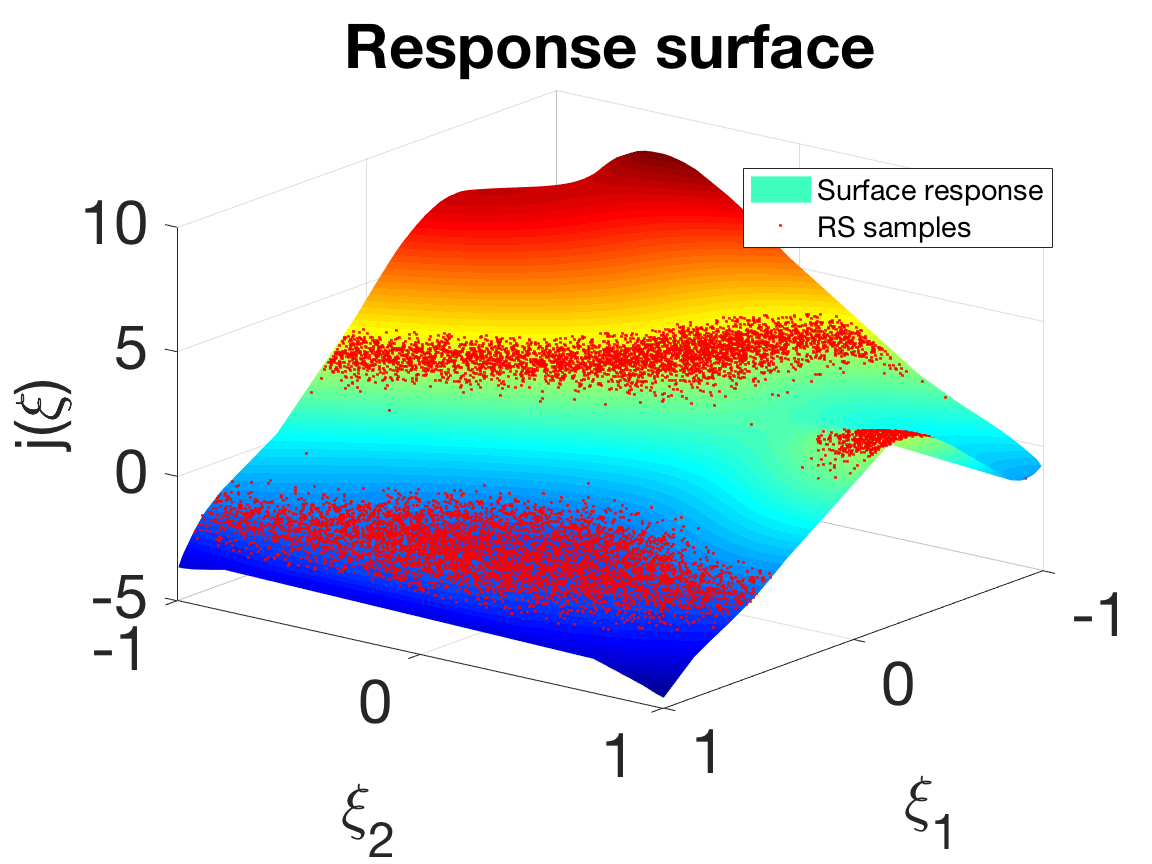
\includegraphics[width=0.5\linewidth]{gPCP5_RS.png}
    {\put(-215,150){\bf (a)}}    
    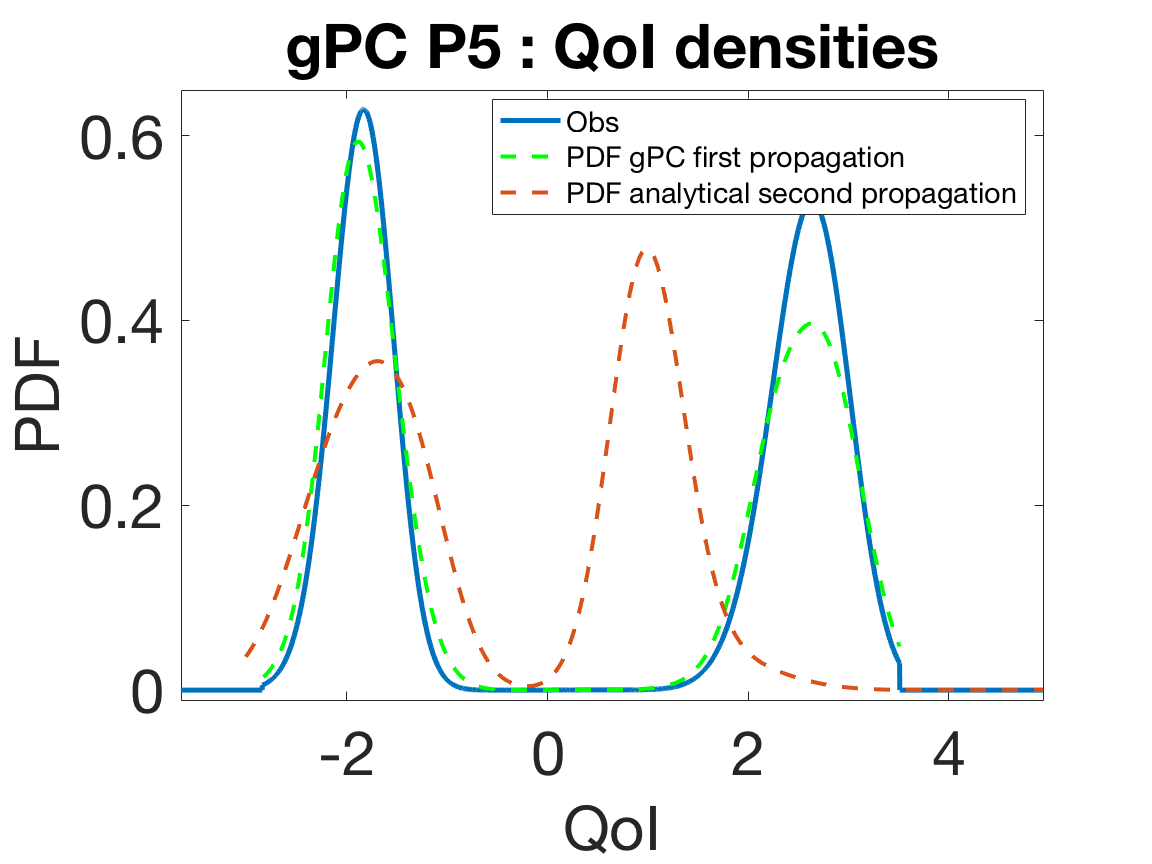
\includegraphics[width=0.5\linewidth]{repgPCp5.png}
    {\put(-215,150){\bf (b)}}
    \caption{\label{gpc} (a) Response surface created with gPC P=5. Red dots are the samples generated by the rejection sampling algorithm (b) blue : observed QoI density, green : rejection sampling samples density on the gPC metamodel (c) analytical rejection sampling samples density}

\end{figure}
gPC results show that polynomials doesn't approach well the discontinuous response surface because of Gibbs oscillations where singularities exist (Fig.\ref{gpc}, left). Nevertheless, samples generated after the inference and rejection sampling algorithm induce a QoI distribution that matches pretty well the observable (Fig.\ref{gpc}, right).
\begin{figure}[htb!]
%
    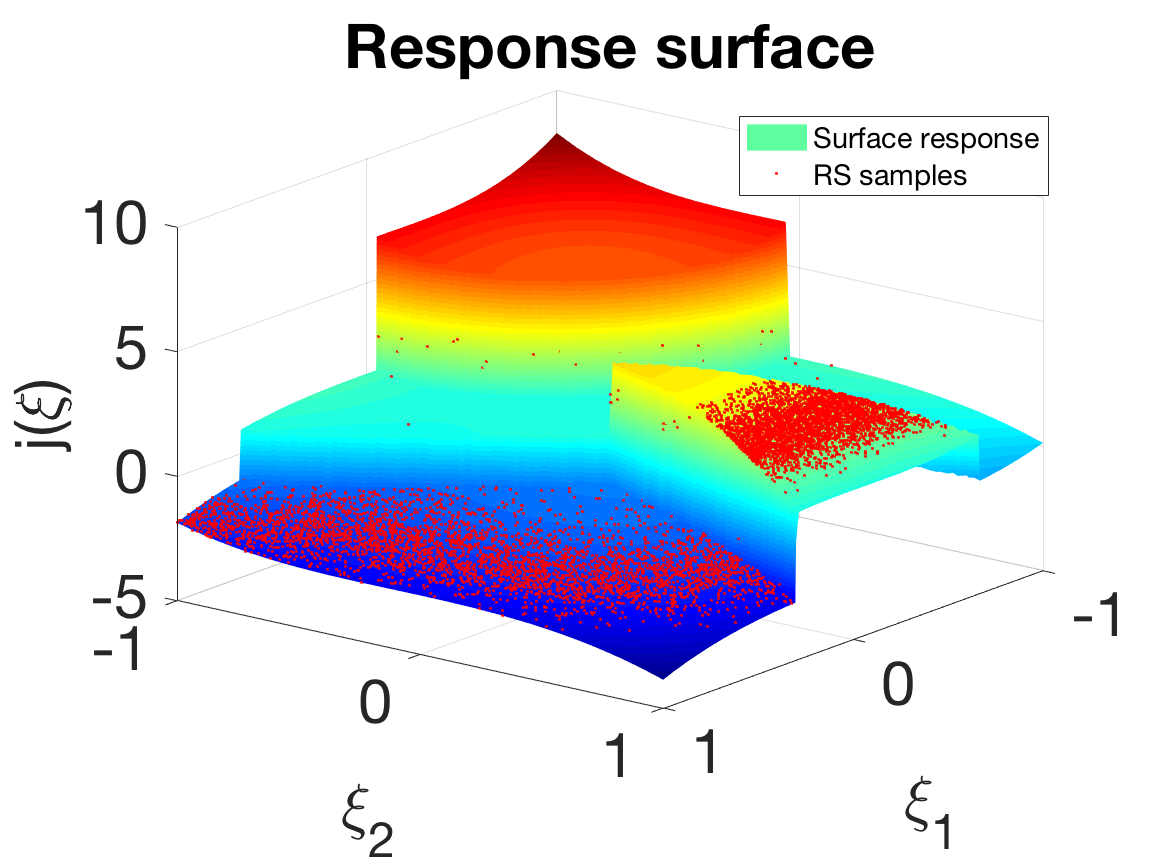
\includegraphics[width=0.5\linewidth]{SC100000_RS.png}
    {\put(-215,150){\bf (a)}}    
    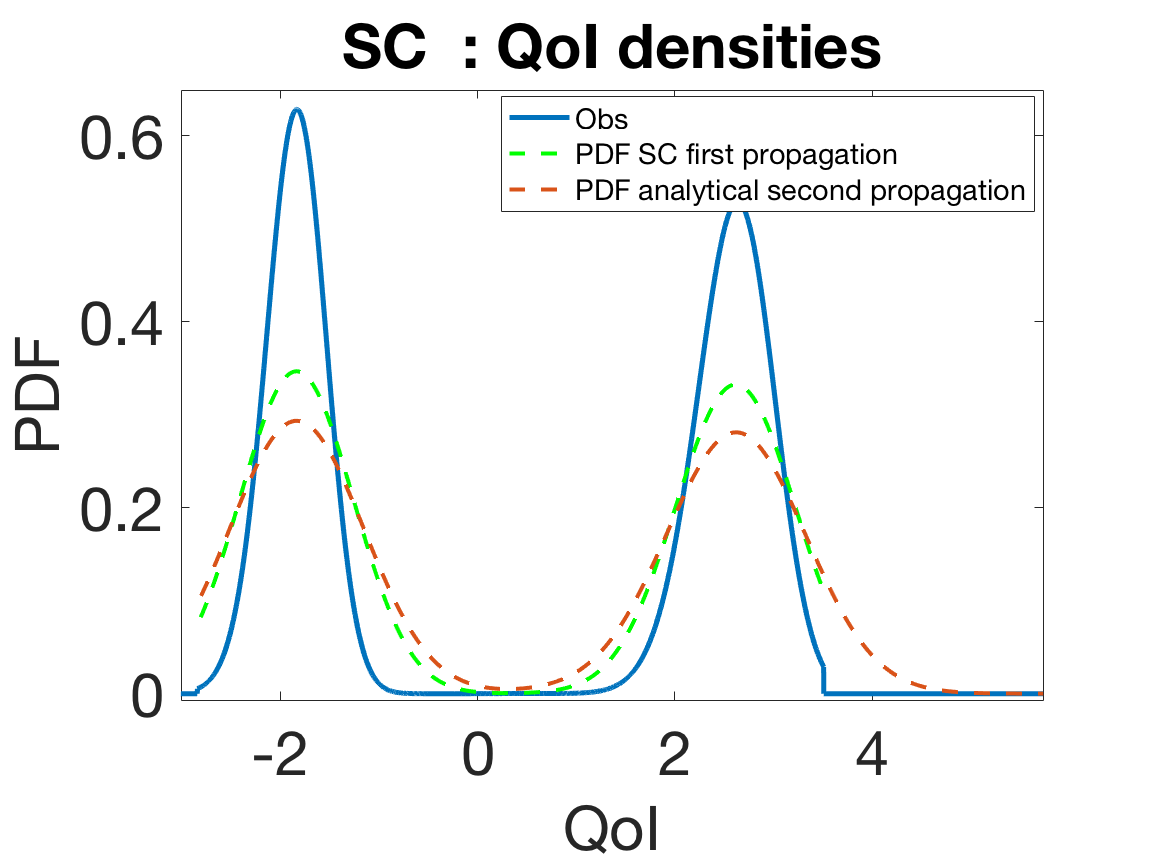
\includegraphics[width=0.5\linewidth]{repSC.png}
    {\put(-215,150){\bf (b)}}
    \caption{\label{sc} (a) Response surface created with the Stochastic Collocation. Red dots are the samples generated by the rejection sampling algorithm (b) blue : observed QoI density, green : rejection sampling samples density on the SC metamodel, red : analytical rejection sampling samples density}

\end{figure}\\\\
Samples computed through the SC metamodel leads to a less accurate QoI density comparing to the one obtained with the gPC (Fig.\ref{sc}). Nevertheless, in order to verify this results reliability we compute the analytical solution for all samples generated by the sampling algorithm ; in both right Figures \ref{gpc} and \ref{sc} the red pdf shows that the SC results are more trustable than the gPC ones. This comes from the worse metamodel approximation using polynomials. More over, the fact that using gPC allows the inference to better work can be understandable since the QoI map is smooth, allowing the inference to get the QoI value it needs. From this observations a new test shall be made, where the observable QoI density should be more representative of the real QoI map computed from $\pi_\Lambda^{obs}$ i.e on the kernel density estimation function used to build the observable.\\\\
\begin{minipage}{0.5\textwidth}
Among all the ksdensity function parameters, the bandwidth is the most important (see appendix, kernel density estimation). The more the bandwidth is small the more the density computed overfits the data. Since the hypothesis is that the previous observable had more information than it should have, we apply the previous methodology to an observable made with a lower bandwidth h=0.01. As shown in the right Figure, when the bandwidth is reduced the density slope changes, getting thinner.
\end{minipage}
\begin{minipage}{0.5\textwidth}
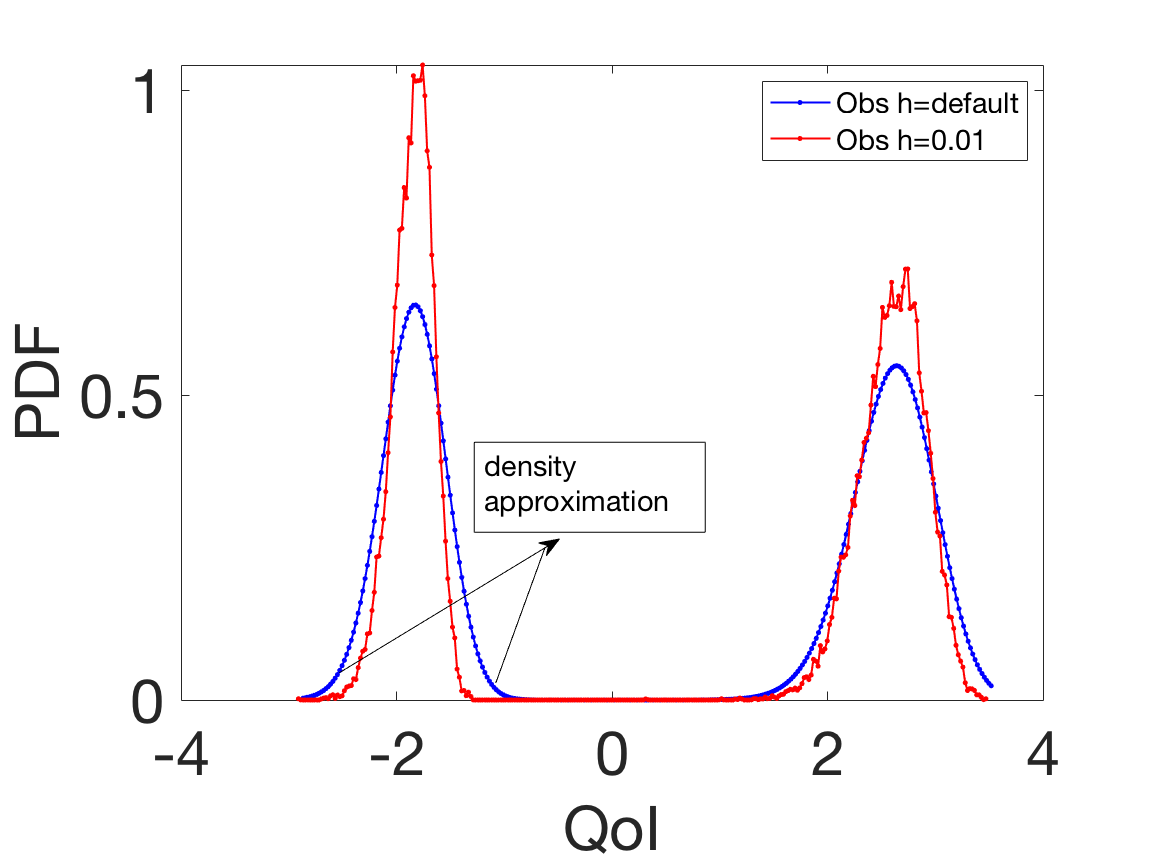
\includegraphics[width=\textwidth]{Obs_bandwidth.png}
\end{minipage}
The hypothesis of "fake observed values" is confirmed where for instance, -1 values were observed previously. We test now the accuracy of gPC and Sc methods.
\begin{figure}[htb!]
%
    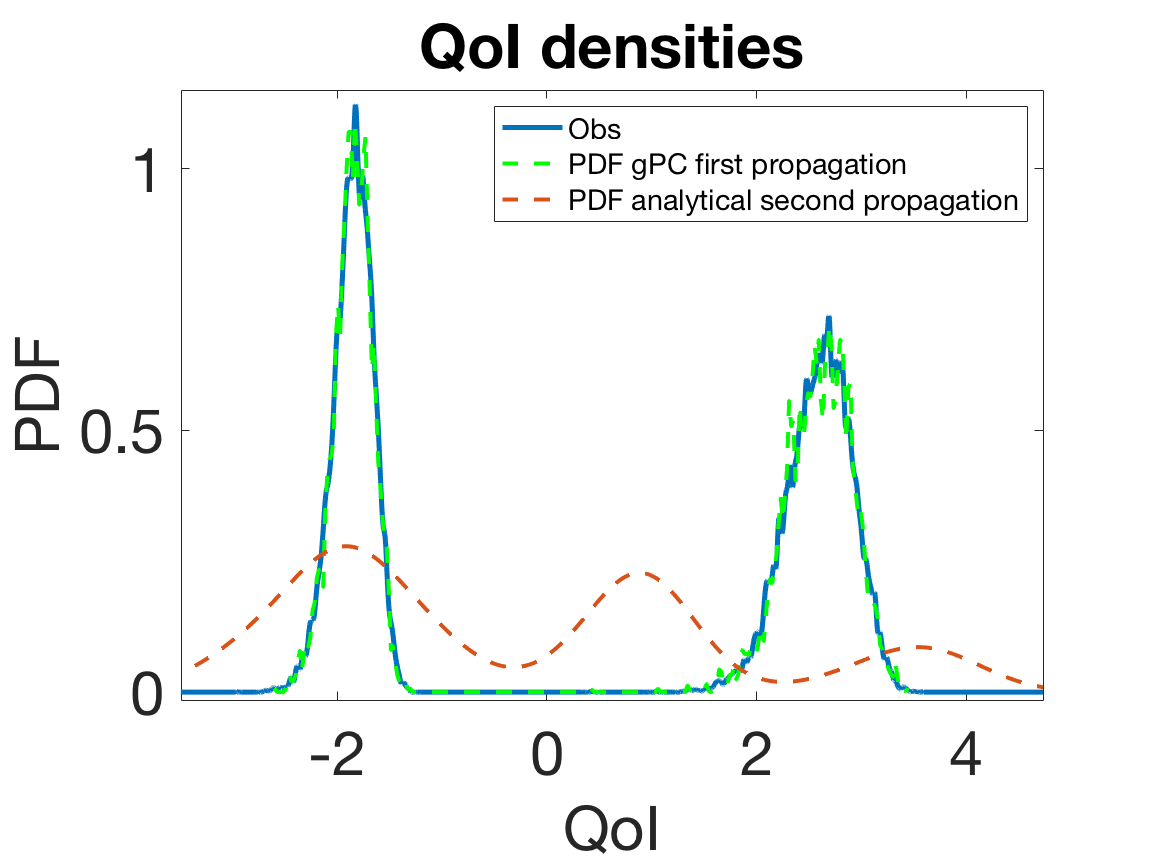
\includegraphics[width=0.5\linewidth]{h001gPCpdf.png}
    {\put(-215,150){\bf (a)}}    
    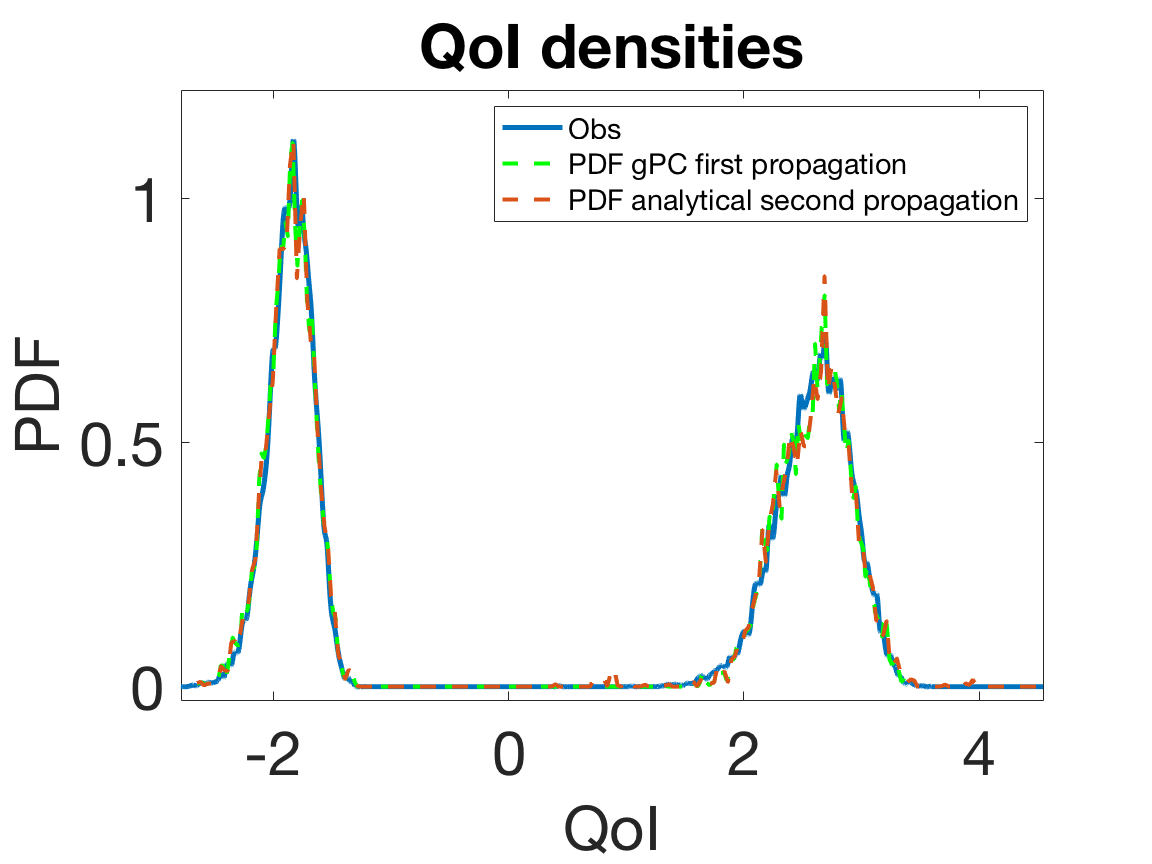
\includegraphics[width=0.5\linewidth]{h001SCpdf.png}
    {\put(-215,150){\bf (b)}}
    \caption{\label{final} blue : observed QoI density, green : rejection sampling samples density on the SC metamodel, red : analytical rejection sampling samples density. (a) gpc (b) SC }

\end{figure}
This time both methods approach the observed density using the inference which is already an improvement from the previous test. When computing analytically the QoI distribution wanted, the forward propagation from gPC samples result in a distribution different from the observed one (Fig.\ref{final}, left). The analytical forward propagation on SC rejected samples bring a very similar distribution from the one obtained during the first inference : it is more accurate than the gPC. Thus, to get a logical result, the band width has to contain the less fake information possible which would lead to a bad posterior. More over, in case of discontinuities in the response surface, we showed that the Stochastic adaptive mesh is able to provide more interesting results than gPC.\\\\
Figure \ref{scdisc} shows the stochastic collocation method efficiency to detect singularities in the QoI map domain. Indeed, comparing 
\begin{figure}[htb!]
%
    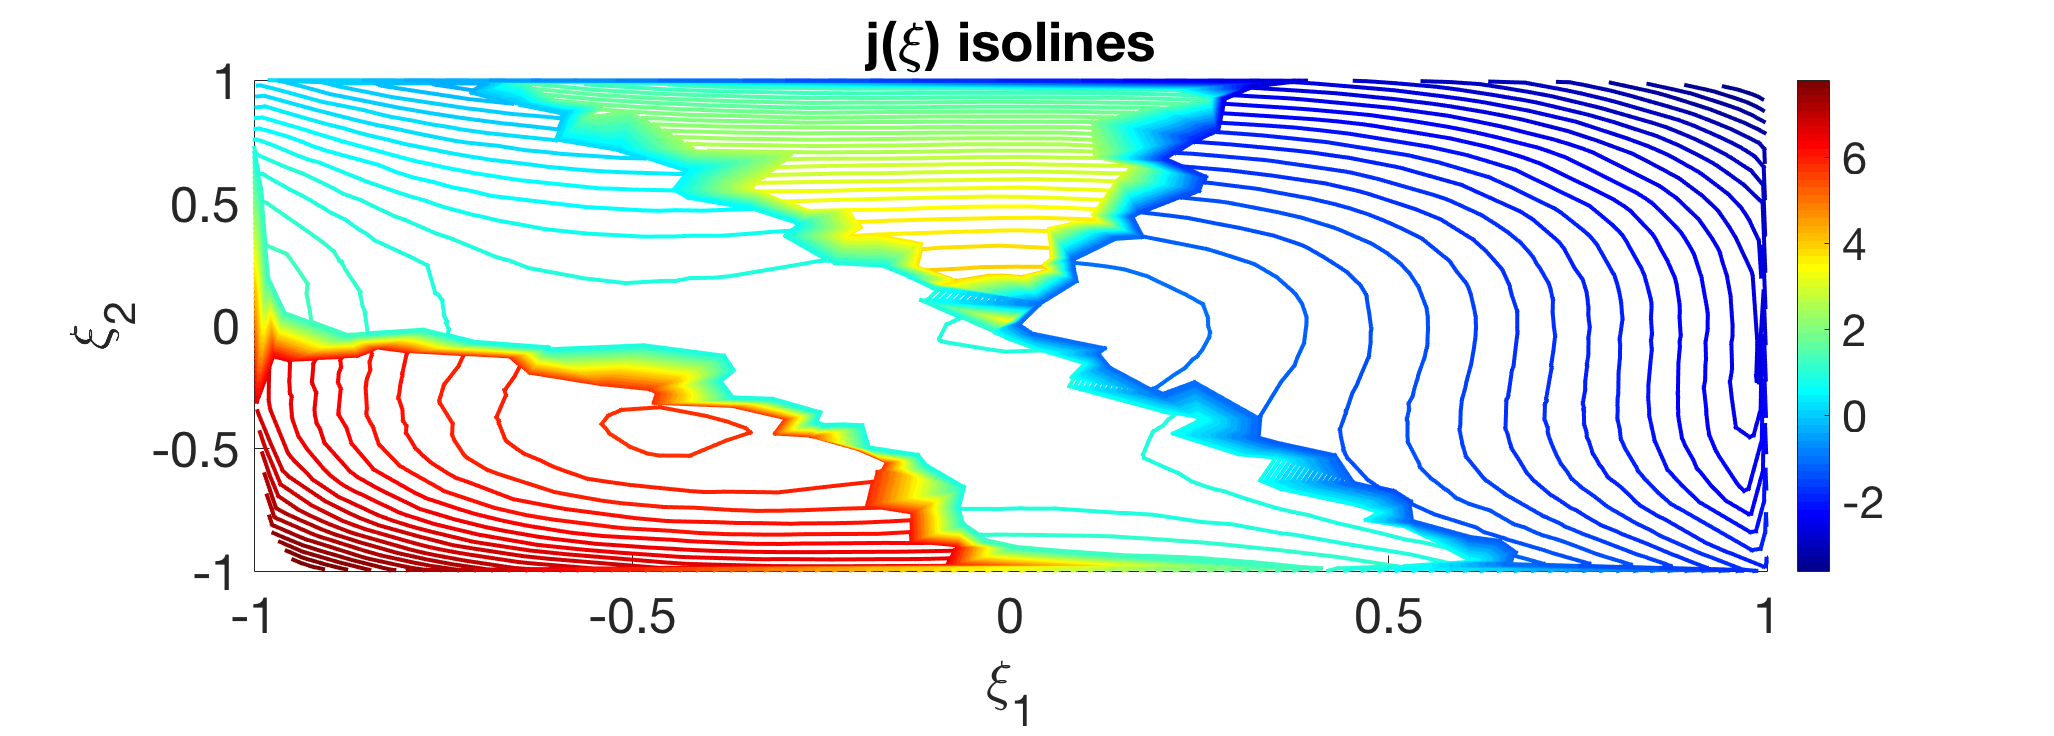
\includegraphics[width=0.9\linewidth]{sx2_MC1e3.png}
    {\put(-215,150){\bf (a)}}    
    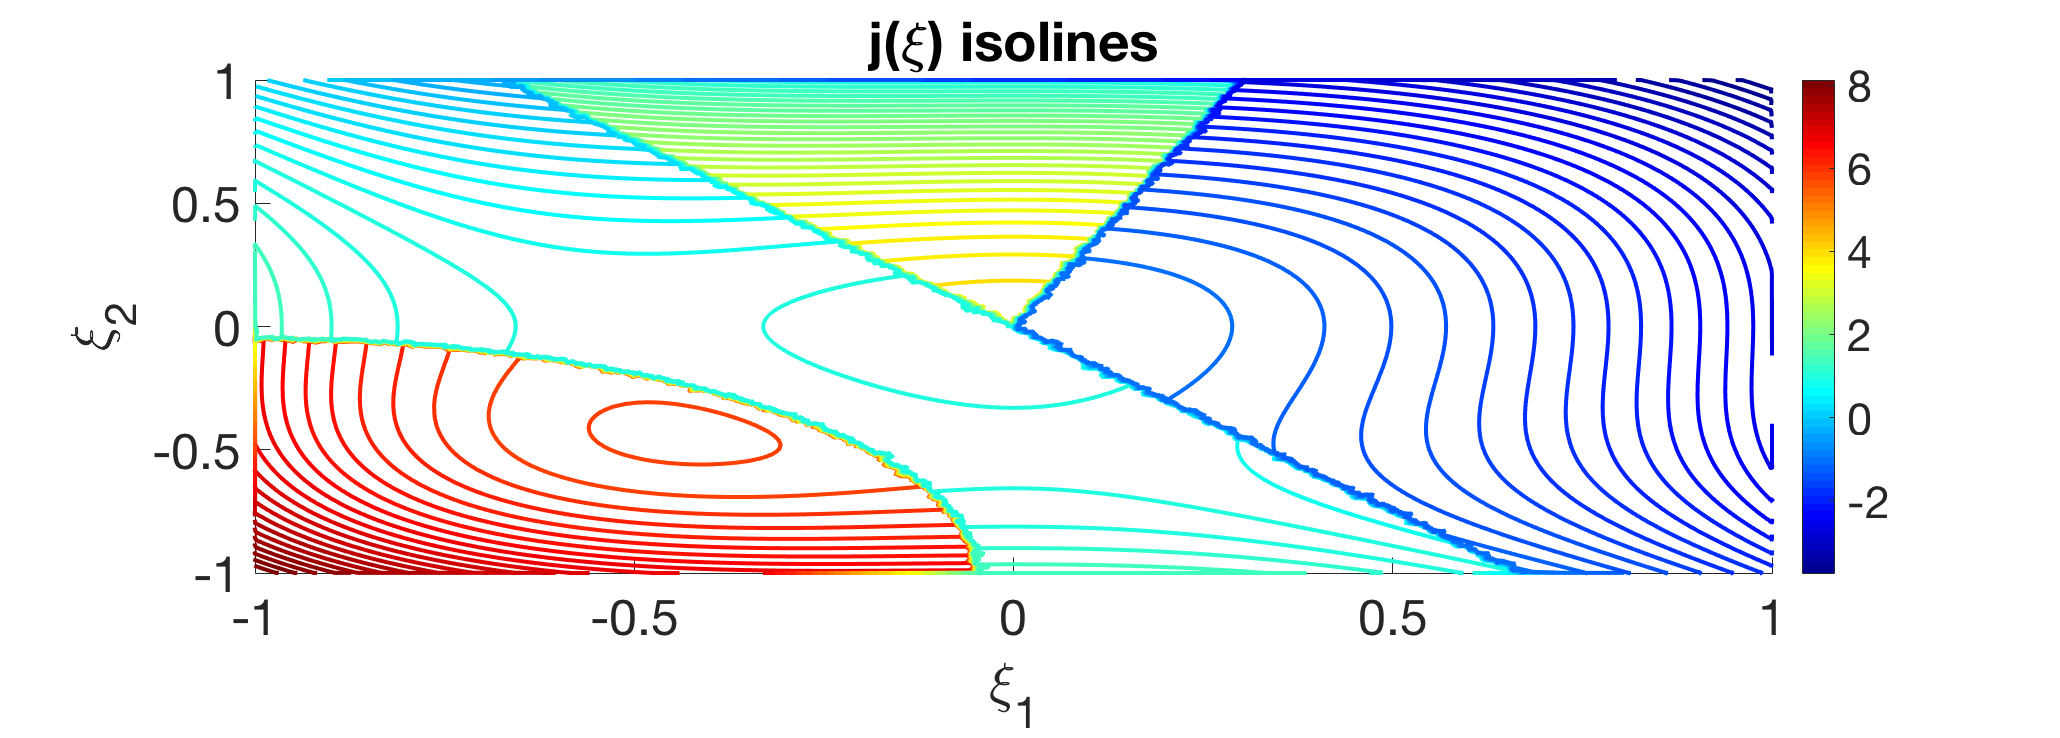
\includegraphics[width=0.9\linewidth]{ex2_MC1e5.png}
    {\put(-215,150){\bf (b)}}
    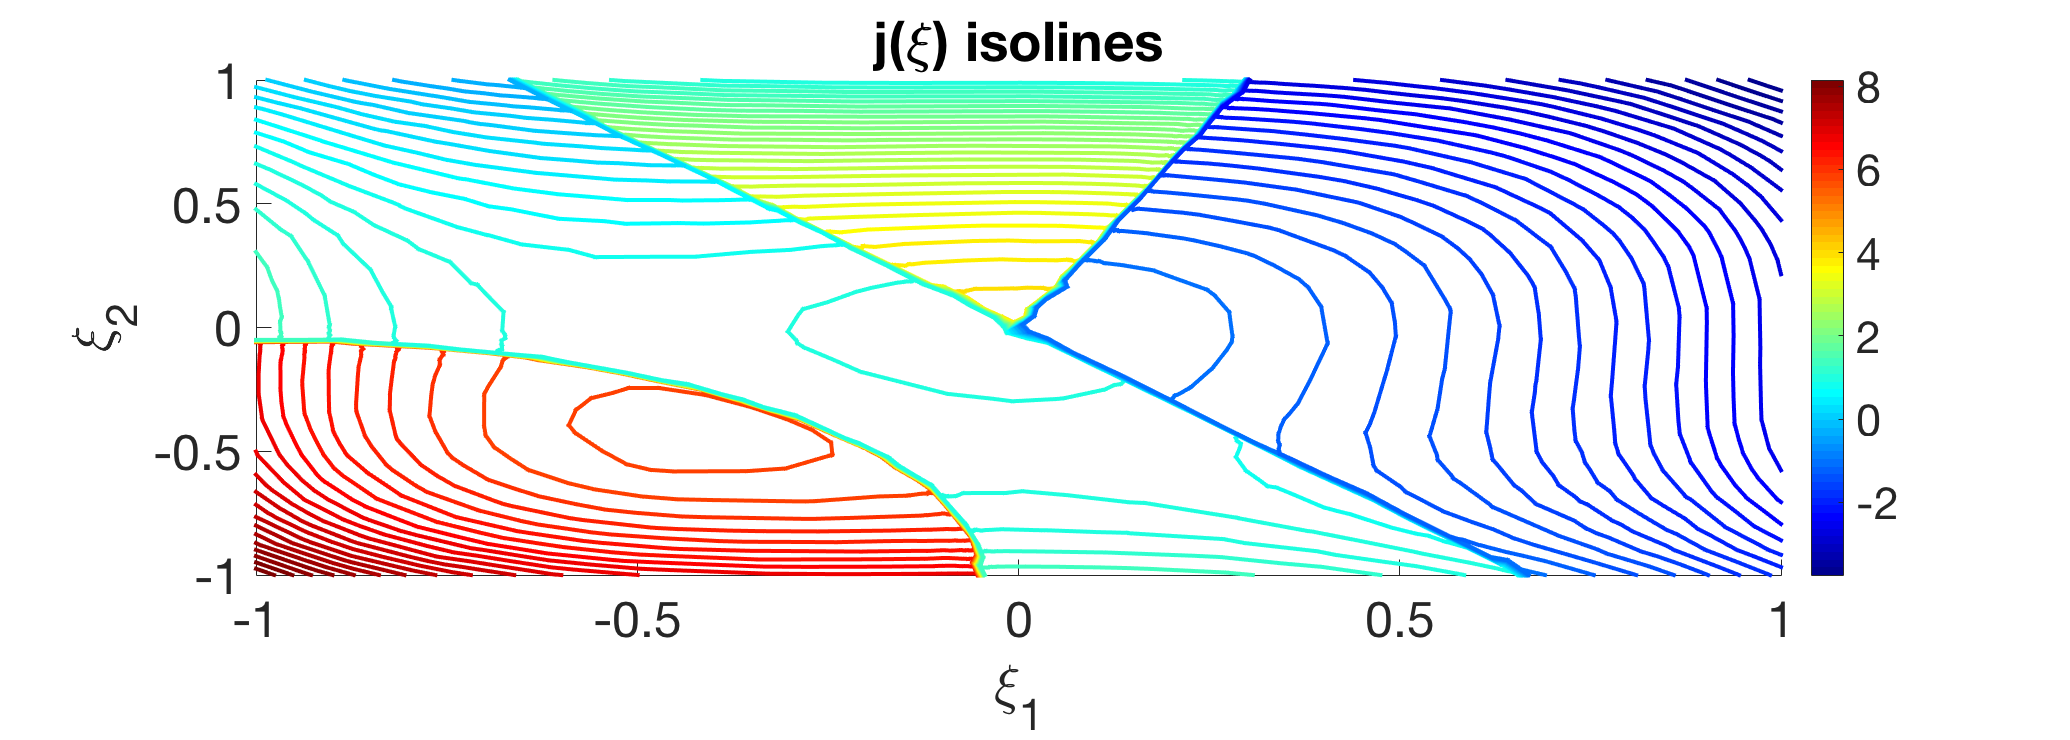
\includegraphics[width=0.9\linewidth]{ex2_SC1e3.png}
    {\put(-215,150){\bf (c)}}
    \caption{\label{scdisc} Isolines of the QoI for example 2. (a) 1e3 MC samples (b) 1e5 MC samples (c) 1e3 collocation nodes (SC)}

\end{figure}

\section{Unicity of the inverse problem solution}
\begin{minipage}{0.5\textwidth}
In order to study inverse CFD problems in a model uncertainty propagation context, we want to evaluate possibilities of applications using the Consistent Bayesian Inference \cite{Tim1}, and better understand on which context this efficient resolution for inverse problems can be used.In the current study, we focus on this method capacity on finding a given type of posterior distribution which was used to built a given quantity of interest (QoI) observed distribution. The next section methodology is applied on the first example presented on 5.4.
\end{minipage}
\begin{minipage}{0.49\textwidth}
    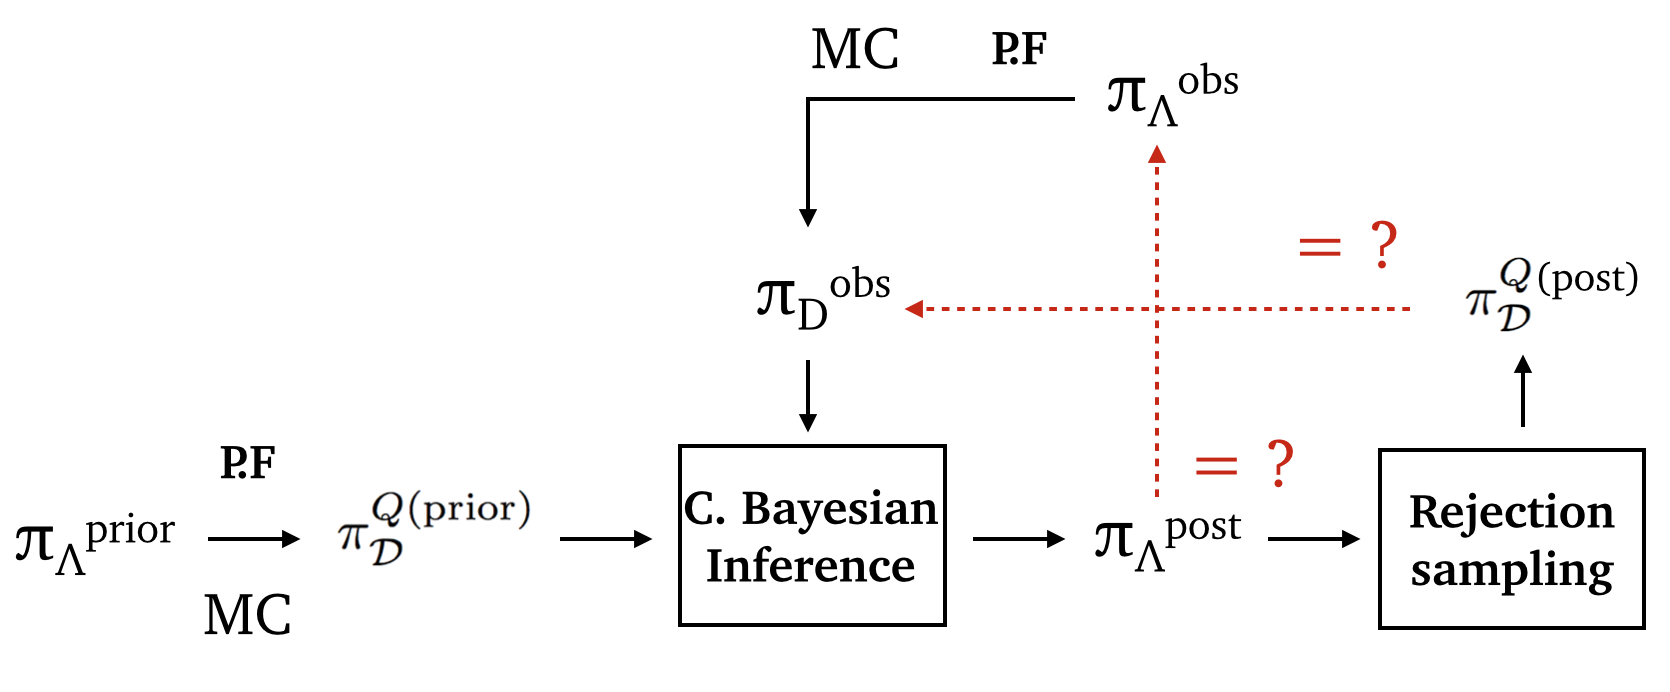
\includegraphics[width=\textwidth]{sch2.png}
    \centering
    \caption{The current study main steps. MC sampling is used to push forward. In red, the final distributions to be compared. $\Lambda$ and $D$ are both sets associated to the uncertain parameters and the model QoI map.}
    \label{sch2}

\end{minipage}

\begin{minipage}{0.5\textwidth}
\subsection{Methodology}
Let $\Lambda$ be the set of the uncertain parameters.
Given a distribution $\pi_\Lambda^{obs}$ in $\Lambda$, we build the QoI map and compute an observed QoI density $\pi_D^{obs}$ using a KDE function  that is used in the Consistent inference. To do so, a prior is then fixed and the inference is made after a Monte Carlo push  forward in the stochastic space. After a rejection sampling algorithm, we compute the posterior QoI map with samples from the first push-forward. Both posterior $\pi_\Lambda^{post}$ and its QoI density $\pi_D^{post}$ are compared to $\pi_\Lambda^{obs}$ and $\pi_D^{obs}$ respectively. Finally, a study on the impact on results of the choice of the prior is made for the first example. The distribution $\pi_\Lambda^{obs}$ used to compute $\pi_D^{obs}$ follows a uncorrelated bi-variate Gaussian with $\mu = [0.9, 1]$, $\sigma_1 =0.001, \sigma_2 = 0.001$.
\end{minipage}
\begin{minipage}{0.49\textwidth}
 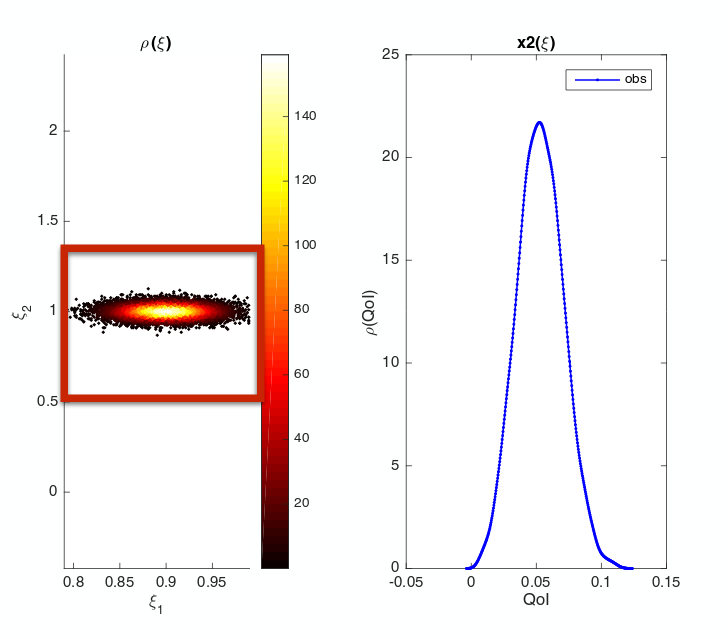
\includegraphics[width=\textwidth]{observable.png}
 \centering
 Left : samples used to compute the observable, right : observable
\end{minipage}\\\\
We want in this study to see if the consistent inference, in addition of matching an QoI observed distribution, can also find exactly the posterior used to its computation. The prior is set as uniform and the forward propagation of all studies here is made with crude Monte Carlo, since we use a simple test case.
\subsection{Results}
For an uniform prior :
\begin{figure}[htb!]
%
    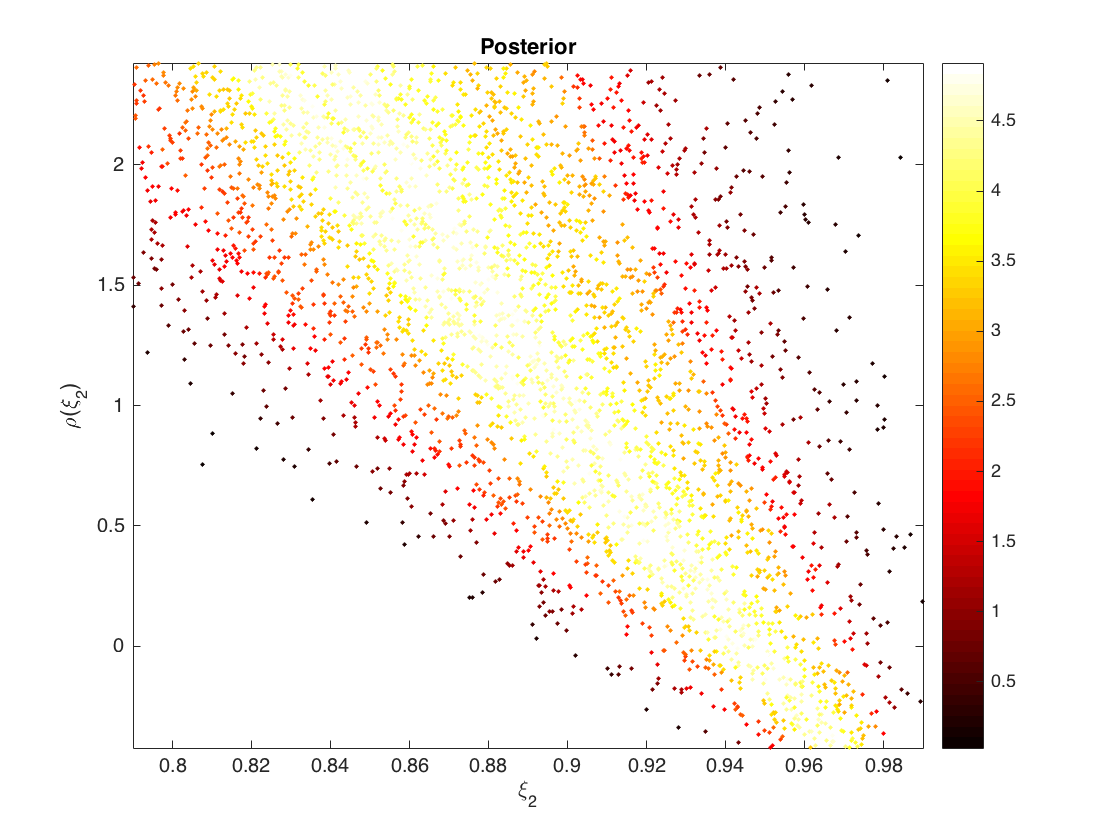
\includegraphics[width=0.49\linewidth]{2Dunipost.png}
    {\put(-215,150){\bf (a)}}    
    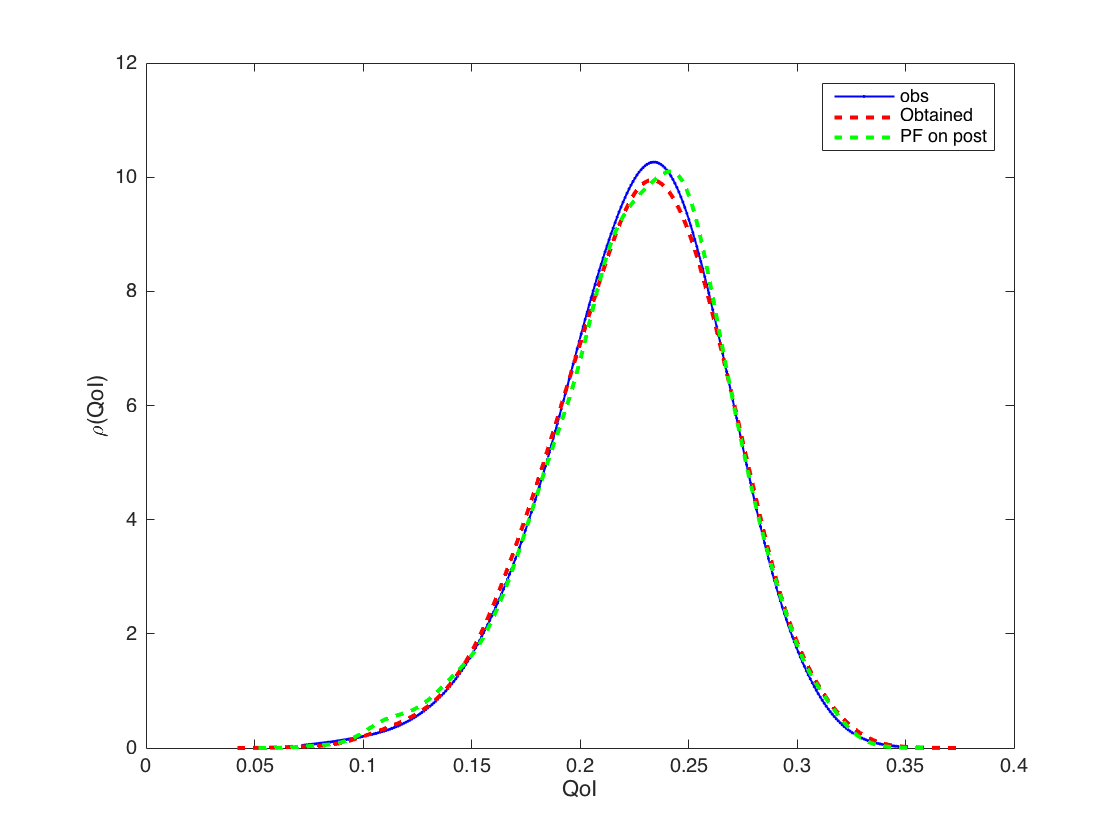
\includegraphics[width=0.49\linewidth]{2Dunipdf.png}
    {\put(-215,150){\bf (b)}}
    \caption{\label{MC1} \textit{The consistent inference results for an uniform prior (a) Posterior computed and represented on samples from the rejection sampling algorithm (b) blue : observed QoI distribution, red : Push forward QoI distribution from rejected samples, green : Independent push forward made in the posterior}}

\end{figure}\\
We observe that despite the fact that the QoI observable is matched, the posterior doesn't match the observed uncertain parameters distribution which makes us question the inverse solution uniqueness. In the reference paper, authors show that for two different type of priors one would compute two different posteriors, that could still match the observable. Thus, a parametric study on the prior is made here in order to evaluate how the computed posterior is affected by the prior choice and if there's a chance, for a given prior, to find a posterior similar to the distribution chosen in $\Lambda$ to compute $\pi_D^{obs}$.\\\\
Prior now follows a Gaussian distribution. In this context, $\sigma_{\lambda_1}$ is set as 0.005, $\mu_{\lambda_1} = 0.89$ and $\mu_{\lambda_2} = 1$. Posteriors are computed following different $\sigma_{\lambda_2}$ values represented in Table \ref{sigma}.
\begin{table}[h!]
\centering
\begin{tabular}{c|ccc}
\hline
Figure 7             & \textbf{(a)} & \textbf{(b)} & \textbf{(c)}\\ \hline
$\sigma_{\xi_2}$ & 0.3 & 0.05         & 0.01         
\end{tabular}
\caption{Values taken by $\sigma_{\xi_2}$}
\label{sigma}
\end{table}\\
\begin{figure}[htb!]
    %  
    \centering
    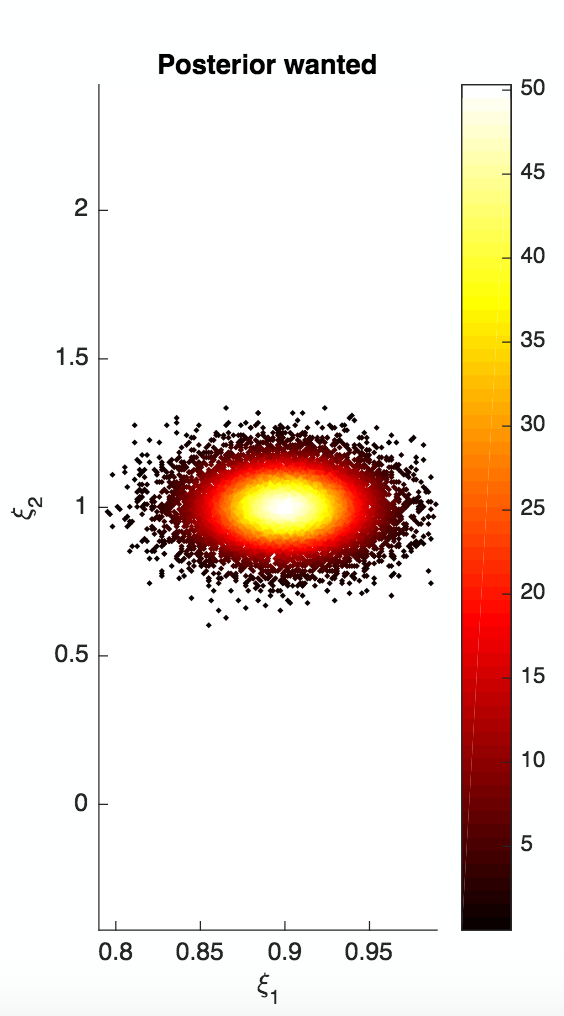
\includegraphics[width = 0.22\linewidth]{1.png}
    {\put(-100 ,170){\bf (a)}}
    %  
    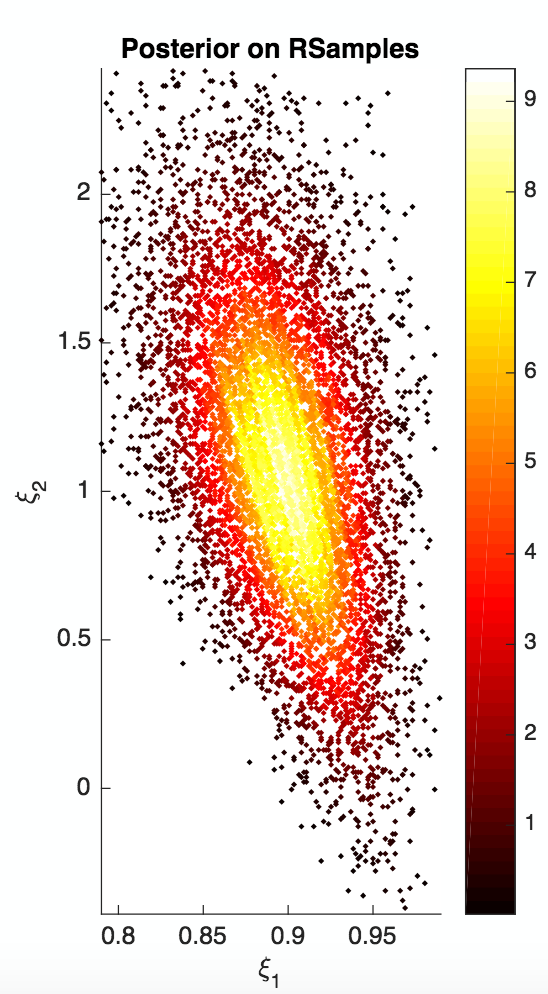
\includegraphics[width = 0.22\linewidth]{2.png}
    {\put(-100 ,170){\bf (b)}}
    %  
    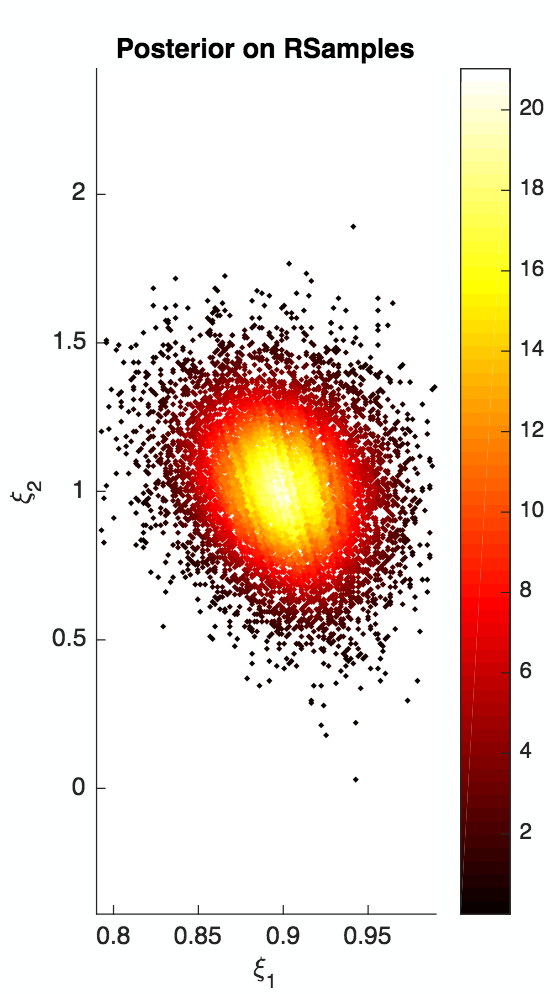
\includegraphics[width = 0.22\linewidth]{3.png}
    {\put(-100 ,170){\bf (c)}}
    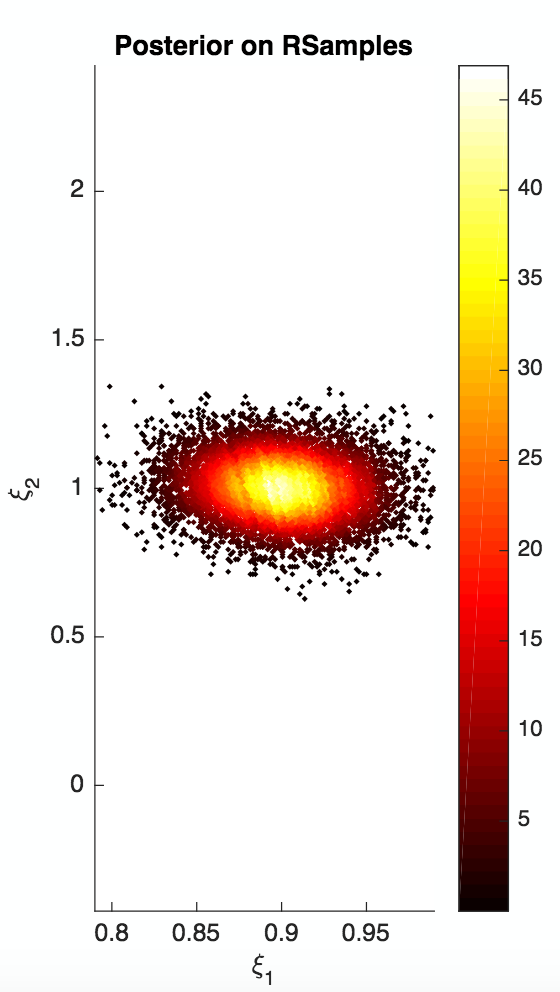
\includegraphics[width = 0.22\linewidth]{4.png}
    {\put(-100 ,170){\bf (d)}}
    \caption{\label{different posterior} Posteriors. (a) Observed (b) $\sigma_{\xi_2}=0.3$ (c) $\sigma_{\xi_2}=0.05$ (d) $\sigma_{\xi_2}=0.01$}
 \end{figure} \\
Results show that the prior choice has as expected an impact on the computed posterior. While the second uncertain parameter variance decreases, we expect to find a final posterior closer to the observed one, which is the case (Fig.\ref{different posterior}). However, one must be aware that sometimes an arbitrary prior choice can be difficult according to the complexity of the studied problem. Although all posteriors computed lead to QoI distributions which match the QoI observable, the closest posterior to the parameters observed one is, logically, the one found with a prior distribution that is also closer to the observable (i.e $\sigma_{\xi_2} = 0.01$) ; therefore, we show here that in order to match $\pi_{\Lambda}^{obs}$ we simplified the problem to a single stochastic dimension. 
\subsection{1 stochastic dimension test}
From this result, we set now, for the example 1, an 1D inverse problem. We keep the QoI as $x_2(\xi)$ and set $\xi_1=0.89$ ($\xi_2 \in [1-4.5\sqrt{0.1}, 1+4.5\sqrt{0.1}])$. With 20 000 MC samples we test the consistent inference. Two priors are compared. First an uniform prior which takes into account all the uncertain parameter ($\xi_2$) stochastic domain, followed by a Gaussian prior with $\mu = 0$ and $\sigma = 0.2$. \\\\
For the first simulation, both QoI and $\xi_2$ distributions computed after the inference match $\pi_\Lambda^{obs}$ and $\pi_D^{obs}$ (Fig.\ref{1D1}). This result is similar the one obtained in last subsection, where the uniqueness of a posterior solving the inverse problem seems to exist. Nevertheless, for the second example, the prior computed (red, left Figure \ref{1D2}), doesn't provide enough information to the inference. As consequence, the post inference QoI distribution doesn't match the observed one. More over the posterior differs of the waited distribution. It's definition in the stochastic domain exist until no more information is provided from the prior. Thus, in future studies the choice of prior is very important ; it must cover at its best the stochastic domain, in order to provide to the inference useful information. Since a 1 uncertain parameter to 1 QoI inference brings an unique solution to the inverse problem, an 2 $\xi$ x 2 QoI study seems to be essential.
\begin{figure}[htb!]
%
    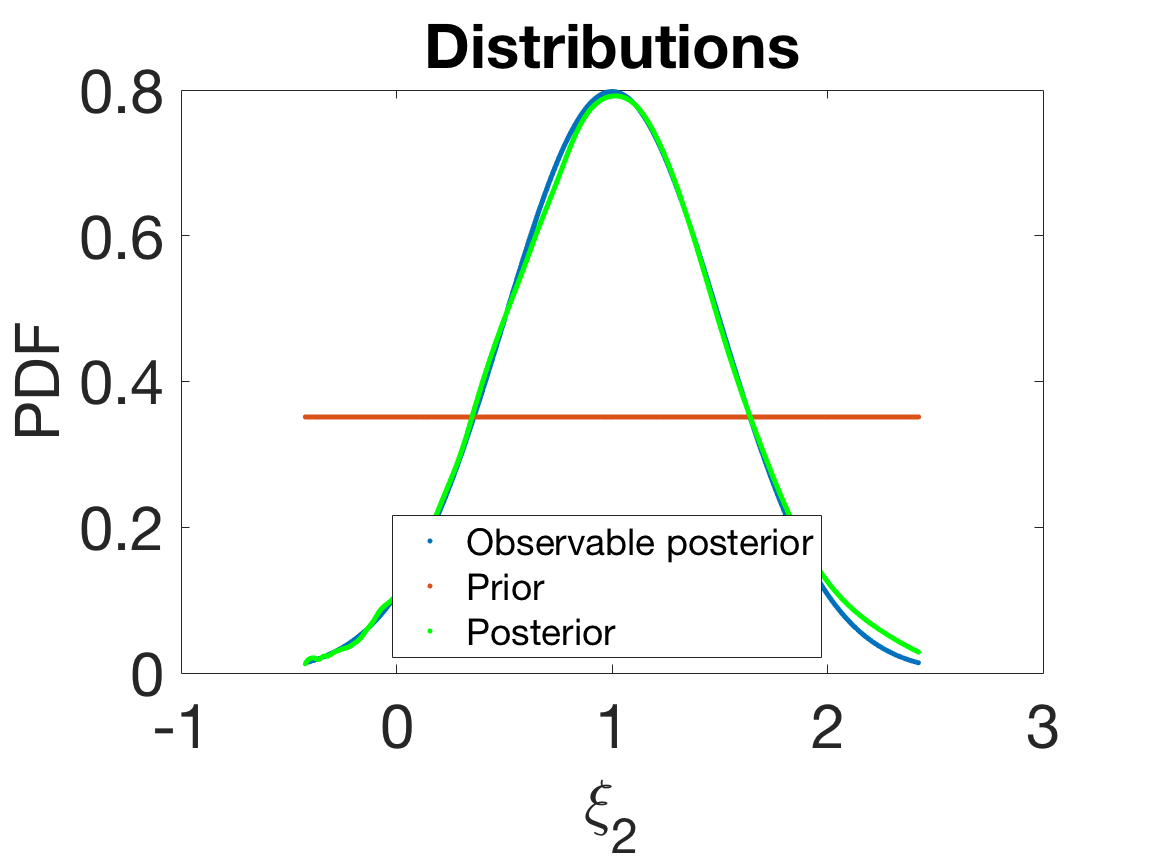
\includegraphics[width=0.49\linewidth]{1Dpost.png}
    {\put(-215,150){\bf (a)}}    
    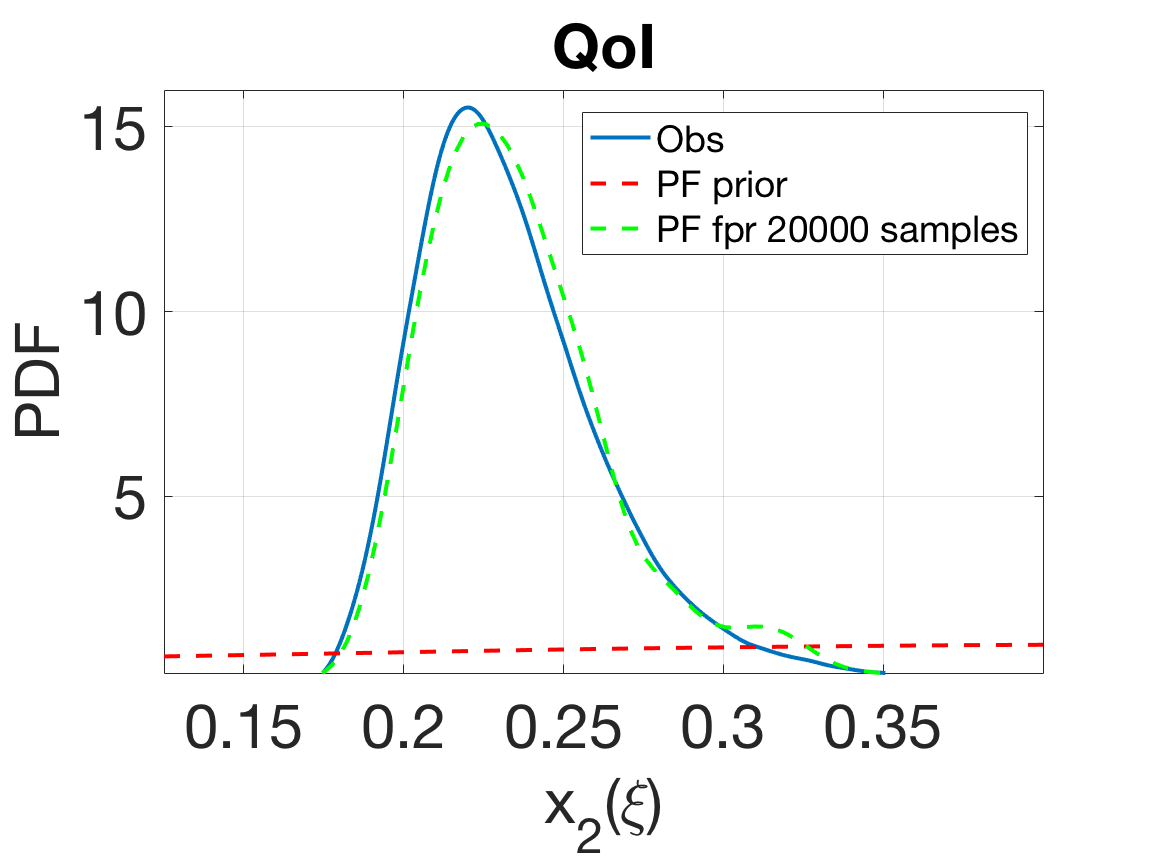
\includegraphics[width=0.49\linewidth]{1Dpdf.png}
    {\put(-215,150){\bf (b)}}
    \caption{\label{1D1} \textit{Uniform prior results (a) blue : Observed distribution, green : Posterior , red : prior (b) QoI distribution. blue : observed, green : RS distribution, red : Prior QoI map distribution} }

\end{figure}
\begin{figure}[htb!]
%
    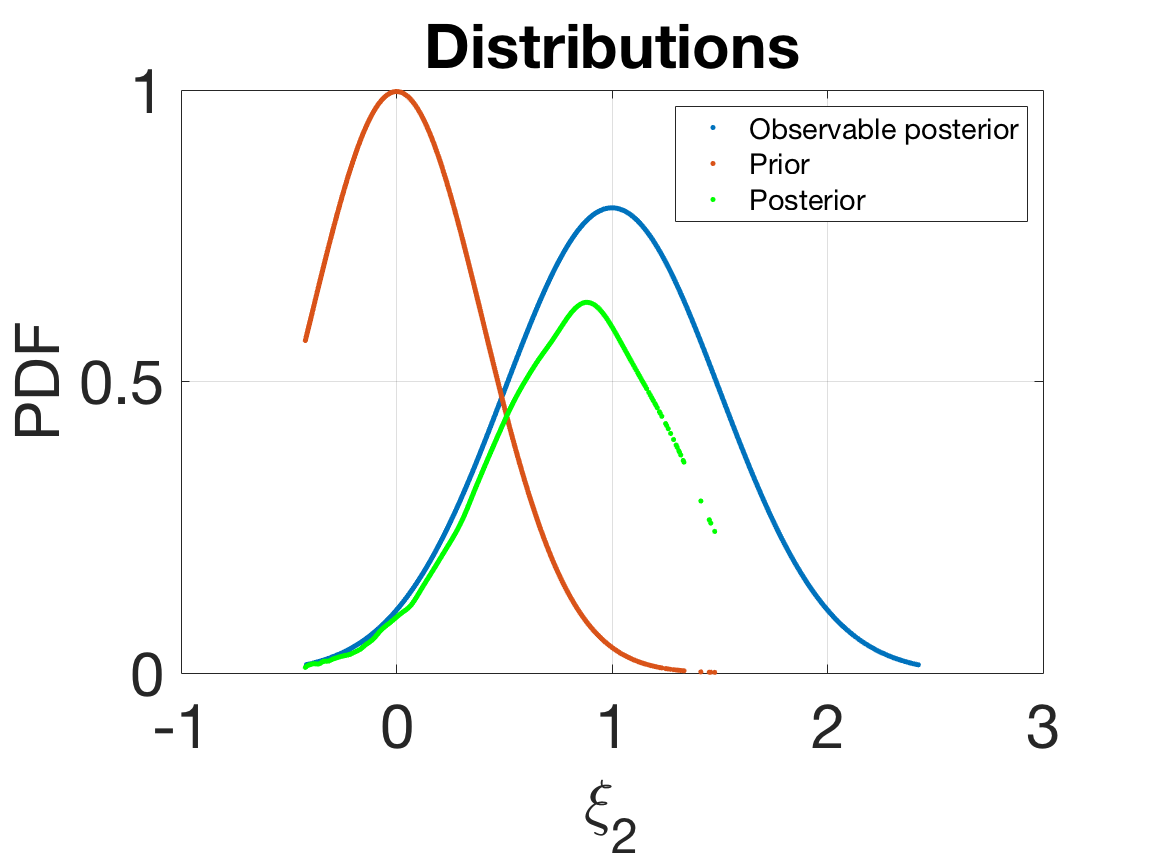
\includegraphics[width=0.49\linewidth]{2e4_post_gaussian2.png}
    {\put(-215,150){\bf (a)}}    
    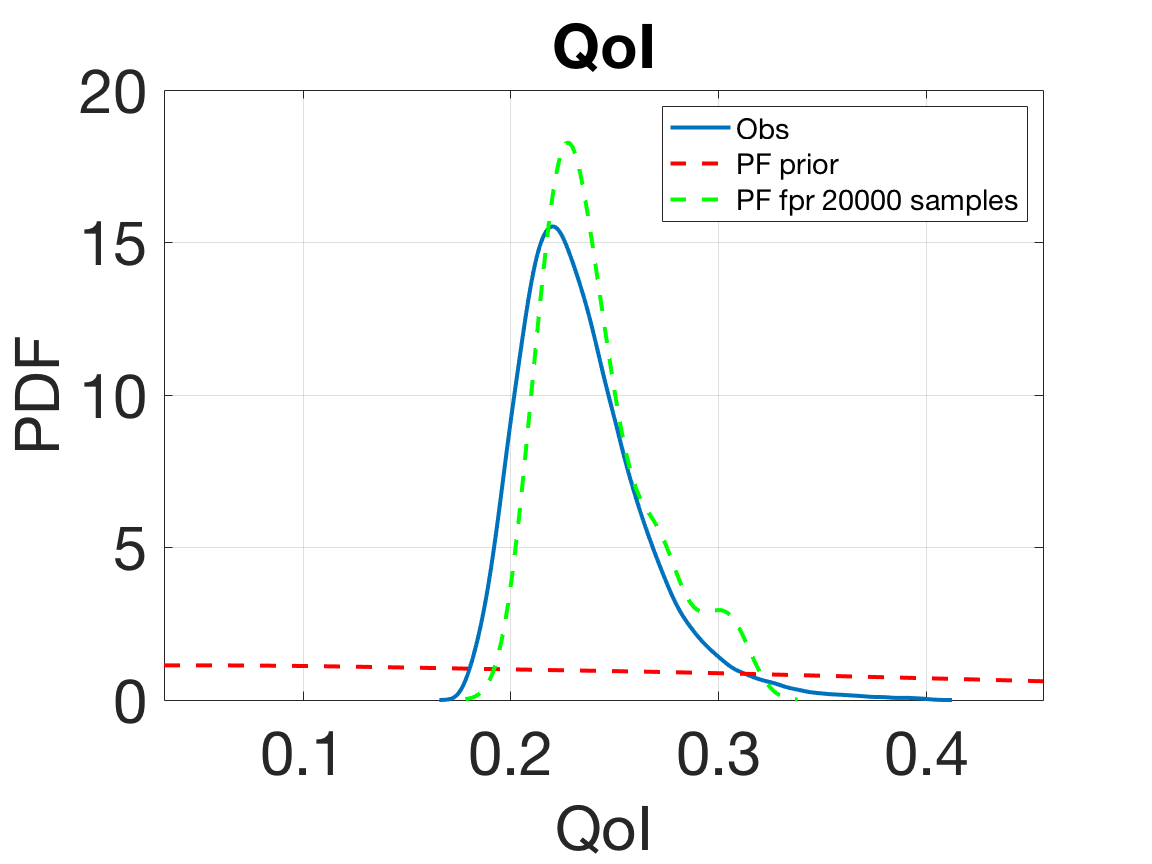
\includegraphics[width=0.49\linewidth]{2e4_pdf_gaussian2.png}
    {\put(-215,150){\bf (b)}}
    \caption{\label{1D2}\textit{N(0, 0.2) prior results (a) blue : Observed distribution, green : Posterior , red : prior (b) QoI distribution. blue : observed, green : RS distribution, red : Prior QoI map distribution}}

\end{figure}
\subsection{2 $\xi$ x 2 QoI test}
For this study we set 2 quantities of interest ($x_1$, $x_2$) for the first example. We apply the same methodology of 6.3.1. The observed QoI density is computed through a forward propagation of a Gaussian bivariate distribution ... and a multi variate kernel density estimation function (left, Fig.\ref{22obs}).
Priors are set as uniform and we use a crude 1e5 samples (the model computing is fast) MC propagation to compute the first QoI map (Fig.) . %METTRE LA FIGURE. 
The posterior is then computed and the final QoI is made after a rejection sampling algorithm. Two main results are observed. First, the consistent inference leads to a QoI distribution which approaches the observed one (right, Fig.\ref{22obs}). More over, unlike the study where the number of QoI was unique, the posterior obtained is very similar to the one used to build the observable and its integral over the stochastic domain is equal to 1.0310. This results are of great importance since its shows the inverse problem uniqueness when the number of uncertain parameters and quantities of interest are equal. Thus, applications for CFD problems can be more easily found from these results. For instance, thanks to the solution uniqueness, we are able to find a stochastic domain which leads to a given QoI observable and then , using a forward propagation, obtain unknown information which couldn't be acquired from experimental tests.
\begin{figure}[htb!]
%
    \includegraphics[width=0.49\linewidth]{Obs_22}
    {\put(-215,150){\bf (a)}}    
    \includegraphics[width=0.49\linewidth]{QoI_pdf_22.png}
    {\put(-215,150){\bf (b)}}
    \caption{\label{22obs}\textit{Quantities of interest (x1, x2) distribution. (a) Observed distribution (b) Distribution computed from the rejection sampling algorithm after the consistent inference}}

\end{figure}

\begin{figure}[htb!]
%
    \includegraphics[width=0.49\linewidth]{distribution1}
    {\put(-215,150){\bf (a)}}    
    \includegraphics[width=0.49\linewidth]{distribution2.png}
    {\put(-215,150){\bf (b)}}
    \caption{\label{22obs}\textit{(a) QoI distribution after the first MC propagation (b) Comparison between the distribution used to build the observed distribution (left) and the posterior computed by the consistent inference (right) }}

\end{figure}
Since the solution uniqueness seems to exist in a 2D smooth QoI response surface, we add some complexity to the problem using now discontinuous QoI response surfaces. To do so, we consider now a first quantity of interest following the example 2 from previous chapters. 
\begin{figure}[htb!]
%
    \centering
    \includegraphics[width=0.49\linewidth]{isoline_q.png}
    {\put(-180,120){\bf (a)}}    
    \includegraphics[width=0.49\linewidth]{isoline_G.png}
    {\put(-180,120){\bf (b)}}
        \includegraphics[width=0.49\linewidth]{distribA.png}
    {\put(-180,120){\bf (c)}}    
    \includegraphics[width=0.49\linewidth]{post_A.png}
    {\put(-180,120){\bf (d)}}
            \includegraphics[width=0.49\linewidth]{obs_A.png}
    {\put(-180,120){\bf (e)}}    
    \includegraphics[width=0.49\linewidth]{pdf_A.png}
    {\put(-180,120){\bf (f)}}
    \caption{\label{std1} \textit{Case A. (a)(b) Isolines (c)(d) Results in $\Lambda$ (e)(f) Results in $D$}}
\end{figure}
\color{blue!40!black}\chapter{CFD applications}
\color{black}
From previous study we found that using the stochastic collocation forward propagation method would bring the coupled forward and backward propagation tool to be more accurate, especially when discontinuities exist in the surrogate model. This chapter shows some uncertainty coupled propagation applications for Computational Fluid Dynamics (CFD) problems. The first study is a localisation study where we evaluate this tool capacity to localise a given domain in the stochastic domain for aeronautics uncertain parameters. We study first the inference capacity to localise a stochastic area with 2 uncertain parameters for a single interest quantity, and then we do a 2 $\xi$ x 2 QoI problem.
\section{Introduction}
All deterministic solutions to the problem were made using the WOLF CFD solver, which is a 2D and 3D Mixed-Element-Volume solvers for compressible Euler and Navier Stokes equations developed at the research center "Institut National de Recherche dédié aux sciences du numérique", INRIA. For first CFD test cases we study different quantities of interest to a NACA 0012 air foil geometry where Euler equations are solved. The mesh used for simulations already existed and is composed of X nodes and is unstructured. For practical reasons, the is refined around the air foil profile, in order to better detect flow impact on quantities such as speed, density or pressure around our shape of interest (Fig.\ref{mesh}).
\begin{figure}[htb!]
%
    \includegraphics[width=0.5\linewidth]{mesh1.png}
    {\put(-225,130){\bf (a)}}    
    \includegraphics[width=0.5\linewidth]{mesh2.png}
    {\put(-225,130){\bf (b)}}
    \caption{\label{mesh} \textit{CFD study domain for the NACA0012 test. (a) Full spatial domain (b) NACA0012 mesh zoom}}
\end{figure}\\
Principal scalar fields are computed such as pressure, the velocity fields and the density one. From these quantities one can evaluate the quantities of interest needed.
\begin{figure}[htb!]
%
    \includegraphics[width=\linewidth]{fields.png}
    {\put(-465,125){\bf (a)}}    
    {\put(-465,110){\bf (b)}}
    {\put(-465,98){\bf (c)}}
    {\put(-440,70){\bf (a)}}
    {\put(-290,70){\bf (b)}}
    {\put(-110,70){\bf (c)}}
    \caption{\label{mesh} \textit{CFD study domain for the NACA0012 test. (a) Full spatial domain (b) NACA0012 mesh zoom}}
\end{figure}\\
\subsection{NACA0012 data settings}
\section{Study 1}
\subsection{Methodology}
\begin{minipage}{0.4\linewidth}
This study aims to evaluate the SC propagation method coupled with the consistent inference in complex problems. Here we don't want to compute a high number of nodes in order to build the metamodel, since the calculation time can be very important. We use the WOLF solver applied to a NACA0012 airfoil profile and create an observed QoI distribution from a specific chosen zone in the stochastic domain. For all studies, the model uncertain parameters are the flow Mach number $M_\infty$ and the angle of attack $\alpha$. These parameter variation are in the following stochastic space $\Lambda=\{[0.5, 0.7], [2,6]\}$. The inference is made in the whole stochastic domain (black square) in order to localize the wanted zone. 
\end{minipage}
\begin{minipage}{0.59\linewidth}
\includegraphics[width=\textwidth]{test_cases.png}

\end{minipage}
\\\\\\
Both posterior $\pi_\Lambda^{post}$ and its push forward density $\pi_D^{post}$ are then compared to the observed ones $\pi_\Lambda^{obs}$ and $\pi_D^{obs}$.
Three different quantities of interest will be studied : the Mach number at x/C = 0.25 and the lift and drag coefficients Cd and Cl. We use the stochastic collocation adaptive mesh to compute each surrogate model (Figure \ref{metamodels}) and a Lunar Hypercube Sampling to propagate uncertainties following $M_\infty$ and $\alpha$. Several studies, with 1 or 2 QoI are made for different stochastic zones. \\\\
The problem will get more and more complex for each study, where first we test the method for a single quantity of interest, then for 2 quantities presenting smooths response surfaces (Cd, Cl). We combine then the Mach number with one of these coefficients, which presents a discontinuous response surface in the flight conditions used. % Est ce qu'on a ajouté une dernière simulation avec 2 response surfaces présentant des discontinuités.
All computed densities from scattered data are made using a KDE function with a bandwidth following  the Silverman's rule of thumb \cite{Silverman} :
$$ b_i = \sigma_i\{\frac{4}{(d+2)n}\}^{\frac{1}{(d+4)}}
 $$
 where d is the total number of QoI, n the number of observations, and $\sigma_i$ is the $i^{th}$ variate standard variation.
% \usepackage{multirow}
\begin{table}[h!]
\centering
\begin{tabular}{|c|c|c|c|}

\hline
\textbf{Study} & \textbf{Quantities of interest} & \textbf{Domain} & \textbf{$\xi$}                      \\ \hline
\textit{1}     & Ma(x/c = 0.25)                  & 1                     & \multirow{5}{*}{$M_\infty, \alpha$} \\ \cline{1-3}
\textit{2}     & \multirow{3}{*}{Cd, Cl}         & 1                     &                                     \\ \cline{1-1} \cline{3-3}
\textit{3}     &                                 & 2                     &                                     \\ \cline{1-1} \cline{3-3}
\textit{4}     &                                 & 3                     &                                     \\ \cline{1-3}
\textit{5}     & Cl, Ma(x/c = 0.25)              & all                     &                                     \\ \hline
\end{tabular}
\end{table}

\begin{figure}[htb!]
%
    \centering
    \includegraphics[width=0.49\linewidth]{CD_meta.png}
    {\put(-140,95){\bf (a)}}    
    \includegraphics[width=0.49\linewidth]{CL_meta.png}
    {\put(-140,95){\bf (b)}}
        \includegraphics[width=0.49\linewidth]{Ma_meta.png}
    {\put(-140,95){\bf (c)}}
         \includegraphics[width=0.49\linewidth]{Ma_lowersurf.png}
    {\put(-140,95){\bf (d)}}
    \caption{\label{metamodels} \textit{Surrogate models used for the CFD studies from two uncertain parameters (a) drag coefficient Cd (b) lift coefficient Cl (c) Mach number on x/c = 0.25 on the upper surface of the NACA0012 airfoil (d) Mach number on x/c = 0.25 on the lower surface of the NACA0012 airfoil }}
\end{figure}
\subsection{Study 1}
\textit{QoI : }Ma(0.25)$(M_\infty, \alpha)$\\\\
In this first study, the zone 1 in the stochastic $\Lambda$ domain is used to build the QoI observable.
We obtain results similar to the study concerning analytical problems with 1 QoI for 2 uncertain parameters. The method isn't able to match the observed distribution in $\Lambda$ : even if the posterior is mostly located in the focused zone and the QoI observed distribution in $D$ is approximated, an important part of $\Lambda$ presents a positive density.
\begin{figure}[htb!]
%
    \centering
    \includegraphics[width=0.49\linewidth]{post_std1.png}
    {\put(-215,160){\bf (a)}}    
    \includegraphics[width=0.49\linewidth]{Unipdf.png}
    {\put(-215,160){\bf (b)}}
    \caption{\label{std1} \textit{Results for study 1. (a) Posterior computed after inference. In blue, the stochastic zone used to build the observable (b) Observed QoI density and post inference density}}
\end{figure}
\subsection{Study 2}
\textit{QoI : }{Cd, Cl}$(M_\infty, \alpha)$\\\\
We test the same methodology but now with two interest quantities (which present booth smooth response surfaces, Fig.\ref{metamodels}). We seek an unique solution in the $\Lambda$ space that corresponds to the choosen stochastic zone used to create $\pi_D^{obs}(Cd, Cl)$. Two different simulations are made. First, $\pi_D^{obs}$ is computed from case 1, then from case 2. For a better understanding of the following results, both QoI iso-contours are represented : 
\begin{figure}[htb!]
%
    \centering
    \includegraphics[width=0.49\linewidth]{Cd.png}
    {\put(-215,160){\bf (a)}}    
    \includegraphics[width=0.49\linewidth]{Cl.png}
    {\put(-215,160){\bf (b)}}
    \caption{\label{iso1} \textit{Iso-contours of the QoI map (a) Cd (b) Cl}}
\end{figure}\\
For the first simulation, the zone used to create the QoI observable (Fig.\ref{simu1}, (a)) is mainly computed by the inference. One can observe that the lower left part of the case 1 stochastic zone isn't fully recognised by the inference (Fig.\ref{simu1}, (b)). More over, this zone is related to a stochastic zone where the drag coefficient map's gradient gets lower (Fig \ref{iso1}, (a)). Consequently, the density computed in the $D$ space doesn't completely match the observable (Fig. \ref{simu1}, (c)(d)). These results could be different and are dependent on the kernel density estimation parameters such as the bandwidth, which will be studied later. 
\begin{figure}[htb!]
%
    \centering
    \includegraphics[width=0.49\linewidth]{distribD.png}
    {\put(-140,95){\bf (a)}}    
    \includegraphics[width=0.49\linewidth]{postcdcl.png}
    {\put(-140,95){\bf (b)}}
        \includegraphics[width=0.49\linewidth]{Obscdcl.png}
    {\put(-140,95){\bf (c)}}
         \includegraphics[width=0.49\linewidth]{pdfcdcl.png}
    {\put(-140,95){\bf (d)}}
    \caption{\label{simu1} \textit{Results for the first simulation, with the observable computed from case 1 }}
\end{figure}\\
Simulation 2 uses the second case zone to build the observable. The inference is then made from all the stochastic domain $\Lambda$.
\begin{figure}[htb!]
    \centering
    \includegraphics[width=0.49\linewidth]{distribcoin.png}
    {\put(-140,95){\bf (a)}}    
    \includegraphics[width=0.49\linewidth]{posterior_coin.png}
    {\put(-140,95){\bf (b)}}
    \caption{\label{postsimu2} \textit{Distributions in the uncertain parameters space. (a) Distribution used to compute the observed QoI density (b) Posterior computed after the inference}}
    \end{figure}\\
     We can see that results are way better, where both observed distributions in $\Lambda$ (Fig.\ref{postsimu2}) and $D$ are well approximated by the consistent inference.
    From both studies we have a first intuition about this method capacity to provide an unique solution to the inverse problem : the iso-contours are shown to have a important impact in results. When selecting a high gradient (mostly for Cd) stochastic zone to compute the QoI observable, we obtain better results, which means that the inference is more able to detect different information in such domains.
\begin{figure}[htb!]
%
    \centering

        \includegraphics[width=0.49\linewidth]{Obs_coin.png}
    {\put(-140,95){\bf (a)}}
         \includegraphics[width=0.49\linewidth]{pdf_coin.png}
    {\put(-140,95){\bf (b)}}
            \includegraphics[width=0.49\linewidth]{cdpdf.png}
    {\put(-140,95){\bf (c)}}
         \includegraphics[width=0.49\linewidth]{clpdf.png}
    {\put(-140,95){\bf (d)}}
    \caption{\label{simu1} \textit{Results for the second simulation in the QoI domain (a) Observed QoI density (b) Post inference computed QoI density (c) Both densities for Cd (d) Both densities for Cl}}
\end{figure}
\subsection{Study 3}
\textit{QoI : }$\{$Ma(0.25) lower surface, Ma(0.25) upper surface$\}$ $(M_\infty, \alpha)$\\\\
In this study we are interested in the Mach number on x/c = 0.25 for both upper and lower surfaces of the Naca0012 airfoil (Fig.\ref{machs}). Those functional of interest present one smooth response surface and another one containing a discontinuity that shall bring more complexity to the inverse problem resolution. The stochastic domain $\Lambda$ is divided in four identical squares (A,B,C,D), such as in \cite{JC}, represented in the Figure  \ref{isolines}. For each zone the coupled tool is tested using an uniform prior in $\Lambda$. The bandwidth used to compute each observed distribution is stored and used by all other kernel densities estimations.

\begin{figure}[h!]
    \centering
    \includegraphics[width=\textwidth]{machs.png}
    \caption{Points where the functional of interest are evaluated}
    \label{machs}
\end{figure}
\begin{figure}[htb!]
%
    \centering
    \includegraphics[width=0.49\linewidth]{Isoline_Ma.png}
    {\put(-210,150){\bf (a)}}    
    \includegraphics[width=0.49\linewidth]{Ma_lower.png}
    {\put(-180,120){\bf (b)}}
    \caption{\label{isolines} \textit{QoI Isolines with all the tested domains. (a) Ma(0.25) isolines (b) Cl isolines}}
\end{figure}
\newpage
\subsubsection{Case A }
\begin{figure}[htb!]
    \centering
        \includegraphics[width=0.49\linewidth]{distribA.png}
    {\put(-180,120){\bf (a)}}    
    \includegraphics[width=0.49\linewidth]{post_A.png}
    {\put(-180,120){\bf (b)}}
\end{figure}

\begin{figure}[htb!]
\centering
            \includegraphics[width=0.49\linewidth]{obs_A.png}
    {\put(-180,120){\bf (c)}}    
    \includegraphics[width=0.49\linewidth]{pdf_A.png}
    {\put(-180,120){\bf (d)}}
\end{figure}

\begin{figure}[htb!]
\centering
        \includegraphics[width=0.49\linewidth]{q1_A.png}
    {\put(-180,120){\bf (e)}}
         \includegraphics[width=0.49\linewidth]{q2_A.png}
    {\put(-180,120){\bf (f)}}
    \caption{\label{std1} \textit{Case A. (a)(b) Isolines (c)(d) Results in $\Lambda$ (e)(f) Results in $D$}}
\end{figure}

\newpage
\subsubsection{Case B }
\begin{figure}[htb!]
    \centering
        \includegraphics[width=0.49\linewidth]{distribB.png}
    {\put(-180,120){\bf (a)}}    
    \includegraphics[width=0.49\linewidth]{post_B.png}
    {\put(-180,120){\bf (b)}}
\end{figure}

\begin{figure}[htb!]
\centering
            \includegraphics[width=0.49\linewidth]{obs_B.png}
    {\put(-180,120){\bf (c)}}    
    \includegraphics[width=0.49\linewidth]{pdf_B.png}
    {\put(-180,120){\bf (d)}}
\end{figure}

\begin{figure}[htb!]
\centering
        \includegraphics[width=0.49\linewidth]{q1_B.png}
    {\put(-180,120){\bf (e)}}
         \includegraphics[width=0.49\linewidth]{q2_B.png}
    {\put(-180,120){\bf (f)}}
    \caption{\label{std1} \textit{Case A. (a)(b) Isolines (c)(d) Results in $\Lambda$ (e)(f) Results in $D$}}
\end{figure}
\newpage
\subsubsection{Case C }
\begin{figure}[htb!]
    \centering
        \includegraphics[width=0.49\linewidth]{distribC.png}
    {\put(-180,120){\bf (a)}}    
    \includegraphics[width=0.49\linewidth]{post_C.png}
    {\put(-180,120){\bf (b)}}
\end{figure}

\begin{figure}[htb!]
\centering
            \includegraphics[width=0.49\linewidth]{obs_C.png}
    {\put(-180,120){\bf (c)}}    
    \includegraphics[width=0.49\linewidth]{pdf_C.png}
    {\put(-180,120){\bf (d)}}
\end{figure}

\begin{figure}[htb!]
\centering
        \includegraphics[width=0.49\linewidth]{q1_C.png}
    {\put(-180,120){\bf (e)}}
         \includegraphics[width=0.49\linewidth]{q2_C.png}
    {\put(-180,120){\bf (f)}}
    \caption{\label{std1} \textit{Case A. (a)(b) Isolines (c)(d) Results in $\Lambda$ (e)(f) Results in $D$}}
\end{figure}
\newpage
\subsubsection{Case D }
\begin{figure}[htb!]
    \centering
        \includegraphics[width=0.49\linewidth]{distribD.png}
    {\put(-180,120){\bf (a)}}    
    \includegraphics[width=0.49\linewidth]{post_D.png}
    {\put(-180,120){\bf (b)}}
\end{figure}

\begin{figure}[htb!]
\centering
            \includegraphics[width=0.49\linewidth]{obs_D.png}
    {\put(-180,120){\bf (c)}}    
    \includegraphics[width=0.49\linewidth]{pdf_D.png}
    {\put(-180,120){\bf (d)}}
\end{figure}

\begin{figure}[htb!]
\centering
        \includegraphics[width=0.49\linewidth]{q1_D.png}
    {\put(-180,120){\bf (e)}}
         \includegraphics[width=0.49\linewidth]{q2_D.png}
    {\put(-180,120){\bf (f)}}
    \caption{\label{std1} \textit{Case A. (a)(b) Isolines (c)(d) Results in $\Lambda$ (e)(f) Results in $D$}}
\end{figure}
\subsubsection{Discussion and conclusion}
%%%%%% APPENDIX %%%%%%%%%%%%%%%
\begin{appendix}
\color{blue!40!black}\chapter{The stochastic adaptive collocation intuition}\color{black}
\section{Introduction and methodology}
This chapter aims to show the computational intuition and results of the stochastic collocation method and the consistent inference. Main reasons to use an adaptive collocation technique comes from some methods difficulties of considering non independent parameters of the used model. More over, metamodel methods such as the gPC have difficulties catching discontinuous QoI response surfaces. Thus, two examples are studied ; one using correlated input parameters the other with a discontinuous response surface. % METTRE LE SCHEMA DE LA FORWARD PROP
\begin{figure}[h!]
    \centering
    \includegraphics[width=\textwidth]{schfp.png}
    \caption{Main steps of a forward propagation using the Stochastic Collocation method. From a initial parameters distribution $\rho_\xi$ a first mesh is computed. After a first evaluation of $j(\xi)$ through the model, the algorithm add new vertices in the stochastic mesh thanks to a error minimisation problem in the Riemannian metric. The final mesh is used to build the QoI map that leads to the QoI distribution $\rho_{j(\xi)}$. This pdf brings to the user useful information of the impact of the model parameters uncertainties on the observed result.}
    \label{SCschema}
\end{figure}
\section{Stochastic correlated parameters}
Given two uncertain parameters $\boldsymbol{\xi} = \{u, p\}$ the Webster function is :
$$ f(u,p) = u^2 + p^3$$
Since one can face complex problems where the random parameters $\boldsymbol{\xi}$ are correlated, an option implemented in the algorithm which uses the correlation matrix between two RV A and B
$$\begin{pmatrix} \sigma_A^2 & \rho\sigma_A\sigma_B \\ \rho\sigma_A\sigma_B & \sigma_B^2 \end{pmatrix}  $$
can be activated as such manner that the multi variable probability distribution function is computed and applied in the model. For the same function we run the iterative process adding the correlated multi variable pdf (where $u$ follows now a Gaussian law $\mathcal{N}(5,0.7)$, p follows a normal distribution $\mathcal{N}(2, 1)$ and $\rho = 0.7$ ) and get :
\begin{figure}[h!]
    \begin{minipage}[t]{0.5\textwidth}
        \centering
        \includegraphics[width=\textwidth]{Webster_cor1.png}
      (a)
    \end{minipage}
    \begin{minipage}[t]{0.5\textwidth}
        \centering
        \includegraphics[width=\textwidth]{Webster_cor2.png}
       (b)
    \end{minipage}
    \caption{Results for the Webster function using correlated random variables distributions. (a) Final response surface and mesh. (b) Quantity of interest pdf.}
\end{figure}\\
The correlation seems to be well evaluated and so do the stochastic mesh adaptation, where vertices are added where the random variables probability is higher. Now that the process main idea is understood let's apply it to more complex problems. 
\section{Discontinuous response surface}
This classic test case is inspired by the work of Lin, Su and Karniadakis \cite{Piston1}, Zhang et al \cite{Piston2}. Later Witteven et al \cite{Piston3} applied simplex elements to the problem and Van Langehoven and al \cite{PistonAnca} tested the current algorithm on it. Here we consider a piston moving in a adiabatic cylinder (a tube) of constant area (Figure \ref{schemapiston}). The tube is filled of air, considered as a ideal gas. As shows the scheme the piston starts at $t=0$ moving to the right at an initial speed $u_{piston}>0$. The associated quantities with the tube at that time are its initial density $\rho_{pre}$, pressure $p_{pre}$ and speed $u_{pre} = 0$
. As the piston moves forward a shock is created and propagate in the tube at $u_{shock}$ speed. Quantities after the shock are indexed as $x_{post}$, with $u_{post} = u_{shock}$. 
\begin{figure}[h!]
    \centering
    \includegraphics[width = 0.8\textwidth]{F1long.png}
    \caption{Piston problem \cite{Piston1}}
    \label{schemapiston}
\end{figure}\\
Since we neglect effects of viscosity, the pressure behind the shock can be calculated with the Rankine-Hugoniot formulation :
$$ p_{post} - p_{pre} = \rho_{pre}c_{pre}(u_{post}- u_{pre})\sqrt{1+\frac{\gamma - 1}{2\gamma} \frac{p_{post} - p_{pre}}{p_{pre}}} $$
with $c_{pre} = \sqrt{\gamma p_{pre}/\rho_{pre}}$ the initial celerity. $\gamma = 1.4$ for air. The shock Mach number can be then calculated \cite{PistonAnca}:
$$ M_{shock} = \sqrt{1+\frac{\gamma + 1}{2\gamma}(\frac{p_{post}}{p_{pre}}-1)}$$
The quantity of interest here is the instantaneous mass flow $m(t)$ placed in a L distance from the initial piston position. Its expression depends on the relative shock position to the sensor :
$$ m(t) = \left \{
\begin{array}{ll}
     \rho_{pre} u_{pre} \mbox{ if } t<\frac{L}{u_{shock}} \\
      \rho_{post} u_{post} \mbox{ if } t>\frac{L}{u_{shock}}
\end{array}
\right.
$$
Lets set $\boldsymbol{\xi} = [u_{piston}, p_{pre}]$ our uncertain parameters as we have :
\begin{table}[h!]
\centering
\begin{tabular}{l|l|l|l}
\hline
Variable     & Distribution law & Parameter 1 & Parameter 2 \\ \hline
$u_{piston}$ & Uniform          & 0.622       & 1.56        \\
$p_{pre}$    & Gaussian         & 1           & 0.02       
\end{tabular}
\end{table}

\begin{minipage}{0.5\textwidth}
Results show that the response discontinuity because of the shock is well captured by the adaptive algorithm (Figure \ref{pistonresults1}). MC interpolation error is on the order of $10^{-5}$. More over the quantity of interest final pdf shows two modes corresponding to both interest surfaces before and after the shock (Figure \ref{pdfpiston} (b)). Note that on the initial mesh initialisation the algorithm relies on the parameters distribution, but once the singularity detected the adaptive optimisation will create nodes in that interesting area. These results are similar to those obtained in \cite{PistonAnca} (not totally identical since different $\rho_{\boldsymbol{\xi}}$ were chosen).
\end{minipage}
\begin{minipage}{0.49\textwidth}
%\begin{figure}
 \begin{center}
         \includegraphics[width = \textwidth]{piston1.png}
    \caption{Piston problem results}
    \label{pistonresults1}
 \end{center}

%\end{figure}
\end{minipage}

\begin{figure}[htb!]
%
    \includegraphics[width=0.49\linewidth, height = 5cm]{piston4.png}
    {\put(-220,150){\bf (a)}}    
    \includegraphics[width=0.49\linewidth]{pistonpdf.png}
    {\put(-220,150){\bf (b)}}
    \caption{\label{pdfpiston}Piston problem. (a) Optimal meshes for each main iteration (b) Quantity of interest probability density function}
\end{figure}


\color{blue!40!black}\chapter{Artificial Neural Networks (ANN)}\color{black}
An Artificial Neural network (ANN) also know as neural network is one of many machine and deep learning models used in numerous domains nowadays. It is a computational model able to learn from any kind of information and predict results from unknown data. However, there is no universally accepted definition of a NN \cite{ANNfaq}. For this work, a neural network is considered as a system composed of many simple processing elements operating in
parallel whose function is determined by the network structure, connection strengths, and the
processing performed at computing elements or nodes (Fig.\ref{fig1}) \cite{defANN}.   \\\\
Such model is actually big topic in the technology industry, since it provides accurate predictions in a short time.
Moreover its popularity doesn't stop increasing since data acquisition booms combined with the exponentially growing standard computational power. Indeed, the more data a network can have, the better it will work. This kind of model is used in most of today's active domains \cite{ANNfaq}, such as probabilities, speech or image recognition, marketing and finances. For instance, a recent Google's model based on neural networks allows the Google Assistant, integrated to Google Allo, to participate to phone calls and to automatically make a personalised reply to a message\cite{GoogleAssistant}.
\begin{figure}[h!]
    \centering
    \includegraphics[width=10cm, height=5cm]{nn.png}
    \caption{Visualisation of the structure, connection strengths, and biases of one of the most successful trained ANNs from DeVries et al (2017) able to predict earthquakes \cite{exemple}.}
    \label{fig1}
\end{figure}\\
 Let's understand first why this method is so effective.
The base of a neural network is a neuron, it represents some memory space that will contain an information. ANN's neurons can be compared to the human neurons which the artificial model is based on \cite{Kriesel}: neural networks are a  simplified caricature of this biological complex system (Fig.\ref{compar}).\\\\\\ Approximately 86 billions neurons can be found in the human nervous system. They are connected by synapses, which are also simulated in an ANN. Incoming signals from other neurons or cells are transferred to a neuron by  these special connections. In a neural artificial model, a neuron receives information from others through weights, which are one of the most important contents in such model; it shows the information flow importance between neurons. To sum up, each neuron receives much information of different intensities. An information processing follow the acquisition thanks to an activation function, explained in the next section.\\\\
Neural networks' main advantages are that they can handle many types of data, even missing data. Moreover, the model can be made without a limit number of inputs and outputs, which can be either a number or an image. For regression problems, they can deal with the non linearity of usual problems treated also by their capability of learning with bad or noisy data. Still, to be efficiently accurate, a neural network needs a large amount of useful data and depending on the problem complexity, a heavy computational power.\\\\
Even though ANNs have clearly a lot of positive aspects, we still can find some cons for this model \cite{AnnProcons}. The best known disadvantage is the model black box nature, since that once the network trained, one cannot explain how and why an ANN came up with a certain output. For instance, in a cat image recognition problem, neural networks can overcome many machine learning techniques but we don't know how it did recognise with precision a cat. Thus, for some problems where a decision must be made with an explainable reason, sometimes a neural network isn't the technique to be used. This is why banks usually don't use ANN to predict whether a person is creditworthy, since an ANN response wouldn't be explainable and acceptable.
\begin{figure}[h!]
    \centering
    \includegraphics[width=\textwidth]{s8_5.jpg}
    \caption{Human and artificial neuron comparison}
    \label{compar}
\end{figure}\\
Actually two types of model exist to solve different problems: regression and classification neural networks (Fig.\ref{models}). The main idea is that a regression network will have as output a precise number, for instance, a pollutant emission, whereas the other one is used to classify something, like pattern recognition. Thus, if faced with a discrete or categorical problem, one would use a classification model. If the problem is about finding something real and continuous, a regression network shall be used \cite{Regression}. \\\\
\begin{figure}[h!]
    \centering
    \includegraphics[scale=0.23]{s9_1.png}
    \caption{Representation of types of neural networks}
    \label{models}
\end{figure}\\
Once the network's type chosen, another configuration must be studied, the way the model will learn. In machine learning techniques, the learning part is crucial and must be wisely chosen between being rather supervised or unsupervised. Supervised learning is done using known outputs; each training sample is affected to a label or number. Therefore, supervised learning's goal is to best approximate the relationship between inputs and outputs thanks to an existent database. On the other hand, unsupervised training does not have labelled outputs, so its goal is to infer the natural structure present within a set of data points\cite{Supervised}.
Such model is useful in exploratory analysis, since it relies information that couldn't be easy for a human to rely. In our case, supervised learning is used .
%penser peut etre a mettre une image de unsupervised image clustering
\section{Major components and structure}
As its name shows, neural networks are mostly composed of neurons, also called nodes. Information transfer between each node is made thanks to weights, that gives the intensity between neurons' connection. Before going further let's introduce the concept of layers.\\
A NN has, at least, an input and an output layer. In more complex situations, a hidden layer, composed of several neurons can be added to the network. The Input layer is made of our entrance parameters. It contains the information used to process the problem; for instance, in a regression network aimed to predict someone's cancer probability, inputs can be the person body characteristics and habits. The Output layer is either a number or a category. Weights are then used to connect neurons between each layer; they are usually stored in a Weight vector or matrix \textbf{W}. Depending on the type of network, connections can follow different architectures. In our case, a basic architecture fits the considered problem's complexity. Connections simply link the inputs to the first hidden layer, that is connected to the second, until the output layer \cite{Kriesel}. \\
Furthermore, a network doesn't operate only with weights between layers. Each neuron has also its bias, which is essential during the model's mathematical process. The neuron information acquirement is usually followed by its processing by an activation function. Basically, considering a single node, the activation function is a scalar-to-scalar function that defines a single node's output Table \ref{table}. Many activation functions exist and are used following the  wanted node output. For instance, the sigmoid activation function takes a real-valued input and squashes it to range between 0 and 1, whereas the tanh takes a real-valued input and squashes it to the range [-1, 1]. In output's layer, purelin activation function ($y=x$) is used, as real discrete results must be returned.  

During the learning phase, an error or cost function $C$ is also needed. Different types of cost functions will be presented later, but to summarise, the cost function's role is to measure the performance of a neural network given a training sample prediction and the expected output.\\\\
Different network architectures exist.
The simplest is the single neuron network. Inputs $x_i$ compose the input vector \textbf{X}, and same for outputs \textbf{Y}. The value given by the neuron $a_1$ after data processing is calculated thanks to:
\begin{equation}
\large a_1=\sigma((\Sigma x_i w_i)+b1)=\sigma(\textbf{X}\textbf{W}+b1)
\end{equation}
Where $\sigma$ is the activation function. In a more complex layer composed of $a^i_j$ neurons for several i layers, we can generalise the previous mathematical expression: 
\begin{equation}
\large a^i_j=\sigma_i(X^{i-1}_j w^{i-1}_j+b_j)
\end{equation}
This allows neural networks to deal with several complex problems.  Networks that have more than 2 layers (input and output) are called multi-layer perceptrons MLP. This kind of network will be used because of its capacity to learn non-linear representations (most of the cases the data presented to us is not linearly separable).\\\\ Despite the existence of several other types of neural networks not presented here which are even more complex (competitive networks, convolutional networks...), from now on only feedforward MLP will be considered, since it was the type of network chosen to predict our emissions. In a feedforward network each neuron in one layer has only directed connections to the neurons of the next layer \cite{Kriesel}. Fig.\ref{arch} below summarise the general MLP process: 
\begin{figure}[h!]
    \centering
    \includegraphics[width=\textwidth, height=8cm]{s9_5.png}
    \caption{Example of a feedforward multi-layer perceptron architecture}
    \label{arch}
\end{figure}\\
In this case, the output array $\hat{Y}$ is calculated with the following expression :
$$\large \hat{Y}=\sigma_3(\textbf{W3}.\sigma_2(\textbf{W2}.\sigma_1(\textbf{W1.X}+\textbf{b1})+\textbf{b2})+\textbf{b3})$$

\color{blue!40!black}\chapter{Numerical tools used in this work}\color{black}
\section{Legendre Polynomials}

\section{Quadratures}

\section{Wolf CFD solver}

\section{The Rejection Sampling algorithm}
The rejection sampling is a popular technique that, given a continuous probability density function $\pi(x)$, which, in our case, was obtained using the kernel density estimation, can generate data points following it \cite{rejection}.\\\\
Consider a 1D stochastic problem.
Let us first introduce $M \ge sup_x \frac{\pi(x)}{p(x)}$ where $p(x)$ is a assumed probability distribution we know how to sample on (for instance, a Gaussian). We generate then a random number Y in our parameters range from the known distribution p and another one U from a uniform law between 0 and 1. If $ U < \frac{\pi(Y)}{M.p(Y)}$, we accept the sample (Figure \ref{rejI}). In our model this algorithm is used to generate random samples given a discrete distribution i.e in the first stochastic mesh creation and in the final QoI pdf evaluation (through the ksdensity function applied on a accepted sample).
\begin{figure}[h!]
    \centering
    \includegraphics[width=\textwidth, height = 5.5cm]{rejection-sampling.png}
    \caption{Example of rejection sampling algorithm \cite{rejImage}}
    \label{rejI}
\end{figure}
\section{Kernel Density Estimation}
The Kernel density estimation is a method used to compute a smooth distribution curve from a given discrete dataset. It will be very useful to estimate distributions during back and forward propagation from a given quantity $X(\boldsymbol{\xi})$. Moreover, one can also generate samples from a given database. We can give a more formal definition of a density $\pi(x)$ computed through KDE :
$$ \pi(x)=\frac{1}{nh}\sum_{i=1}^n K( \frac{X_i - x}{h} )     $$
where n is the dimension of our parameters, K is the Kernel function, which is smooth, like a Gaussian, for instance. The kernel function will weight the distances for each point located at a given x (see Figure \ref{kernel2} (d)). h is called the bandwidth and plays a vital role in the final density computation. The more h will be large, the smoother the distribution will get. \\\\
Let us give an example. Consider the following output of interest of a model and its histogram. The KDE will apply the presented formula and estimate a continuous probability density function (Figure \ref{kernel2}). Once the density is computed, we can then use it to estimate any probability in the stochastic domain.
\begin{figure}[htb!]
    %  
    \includegraphics[width = 0.49\linewidth]{kernel1.png}
    {\put(-170,110){\bf (a)}}
    \includegraphics[width = 0.49\linewidth]{kernel2.png}
    {\put(-170,110){\bf (b)}}
    \center
    \includegraphics[width = 0.49\linewidth]{kernel7.png}
    {\put(-170,110){\bf (c)}}
     \includegraphics[width = 0.49\linewidth]{kk.png}
    {\put(-170,110){\bf (d)}}
    \caption{\label{kernel2} (a) Output of interest in a stochastic mesh (b) Its histogram (c) Kernel density estimation for different bandwidths : h = 0.001, h = 0.01, h = 0.03. (d) Intuition on the kernel density estimation. From random generated samples (white circles), and a given bandwidth, the kernel function (curve in red) apply weights to each value.  }
\end{figure}\\

Finally, this scheme is known to converge $\mathcal{O}(N^{-4/(4+d)})$ where d is the number of uncertain parameters dimension \cite{kernelconvergence}.



\color{blue!40!black}\chapter{gPC module validation}
\color{black}
In order to use the generalized polynomial chaos non intrusive method, a gPC module was coded and validated using the non-linear system presented in (donner le chapitre). We proceed the validation methodology presented below for 1D and 2D test cases.
\section{Methodology}
We fix $x_2$ as quantity of interest. The model uncertain parameters are set in the same range from the reference paper \cite{Tim1}. We compare, with MC analytical results, the first and second moments of MC samples where the QoI was computed using the spectral approach. 2nd and 5th degree polynomials are studied and the quadrature used to the spectral projection is Gauss Legendre. Quadrature number of points $N_q$ in 1D follows, for a polynomial degree P :
$$ N_q =\frac{2P+c}{2}$$
where c is a constant which depends on the type of Gauss method used. For instance, c=1 for classical Gauss quadrature, c=2 for Gauss Radau and c=3 for Gauss Lobatto \cite{CoursLucor}. The 2D grid weigths are calculated through tensor product. For this study a uniform distribution is given for the model uncertain parameters. Thus, we use the orthogonal bivariate Legendre Polynomials.
\\\\ 
In the 1D study, we set $x_1$ as 0.89. \\\\
In the 2D study, we add to figures the deterministic quadrature moments to evaluate the polynomial representation convergence. Since the random variable $Y$ is represented with orthogonal polynomials, the two first statistical moments are \cite{CoursLucor} : 
$$\mu =\mathbb{E}[Y] = a_0 $$
and 
$$\sigma^2 = \mathbb{E}[(Y - \mathbb{E}[Y])^2] = \sum_{k=1}^\infty a_k^2\mathbb{E}[\psi_k^2(X)]$$
We expect the moments computed with the spectral projection to converge to those values. More over, two different sampling techniques are applied to the metamodel and the speed of convergence between the Monte Carlo Sampling (MCS) and Latin Hypercube Sampling (LHS) are compared.
\section{Results}
\subsubsection{1D results :} 
From results in 1D, we first observe that a polynomial with higher order approaches better the analytical solution (Fig.\ref{validationgPC1}). Moments results confirm the better approximation using P=5, where both expectation and variance from the gPC MC samples are close to the analytical moments (represented in blue, Fig.\ref{validationgPC2}). Finally, moments seem to convergence to a given value for each polynomial degree as does the crude Monte Carlo moments. 
\begin{figure}[htb!]
%
    \includegraphics[width=0.49\linewidth]{P2.png}
    {\put(-225,150){\bf (a)}}    
    \includegraphics[width=0.49\linewidth]{P5.png}
    {\put(-225,150){\bf (b)}}
    \caption{\label{validationgPC1}Analytical results in red, spectral gPC in blue. Green crosses stand for the Gauss Legendre quadrature points. (a) P = 2 (b) P = 5}

\end{figure}
\begin{figure}[htb!]
%
    \includegraphics[width=0.49\linewidth]{mu.png}
    {\put(-225,150){\bf (a)}}    
    \includegraphics[width=0.49\linewidth]{var.png}
    {\put(-225,150){\bf (b)}}
    \caption{\label{validationgPC2}1D results : (a) First statistical moment (expectation) for MC analytical results, P=2 and P=5 (b) Second statistical moment (variance)}

\end{figure}\\
\newpage
\subsubsection{2D results :} 
For 2D simulations, we'd rather apply Latin Hypercube Sampling instead of Monte Carlo since it brought faster converging results. Similarly to 1D results, we observe that P=5 approaches better the solution. Nevertheless, expectation results show a larger difference between P=2 and P=5 approximation accuracy ; Adding a stochastic dimension brought useful information for the first statistical moment so a lower degree polynomial can approach the solution easier.
\begin{figure}[htb!]
%
    \includegraphics[width=0.49\linewidth]{lhs_mu2D.png}
    {\put(-225,150){\bf (a)}}    
    \includegraphics[width=0.49\linewidth]{lhs_sigma2D.png}
    {\put(-225,150){\bf (b)}}
    \caption{\label{validationgPC1} 2D results (a) First statistical moment (expectation) for MC analytical results, P=2 and P=5 (b) Second statistical moment (variance)}

\end{figure}

\color{blue!40!black}\chapter{Minimization of the stochastic error}\color{black}
\section{Error Estimation}
This section introduces the notion of total error and splits it into two following the deterministic and stochastic sources. 
\\\\
In cases where the quantity of interest response to the random input parameters is smooth, popular methods such as gPC and the stochastic collocation are efficient. Nevertheless, when the response possesses discontinuities and is of low regularity, global polynomials approximation suffer from Gibbs oscillations \cite{Janthesis}. One possible solution is to divide the space in sub-domains where a local polynomial approximation is made, also called a multi element method. Different works focused on making an adaptive stochastic sampling refinement ; Giovanis and Shields \cite{Giovanis} focused on a variance based SSC where the refinement is informed by variability in the solution of the
system. The method was applied to several stochastic systems and comparisons between classic SCM and the SSC showed improvement in results' accuracy.\\\\
This work main goal is to get the more robust response surface for a quantity of interest. This precision relies on both model's solution and the uncertainty propagation robustness. Thus, in order to have an accurate control of our error we may separate it according to its different sources. Let's define the model our solution depends on $\Psi$ (for example the Navier-Stokes system), having $w(\boldsymbol{\xi},x)$ for exact solution. Note that the exact wording doesn't refer to an unique and fully exact solution, but rather to a solution the freest possible of numerical errors, since an exact solution is out of reach in real life complex problems such our. Thus, at a given computational cost after a spatial discretization $\mathcal{H}_{h_x}$ we can have an approximate solution of $\Psi(\boldsymbol{\xi}_{(i)},w(\boldsymbol{\xi}_{(i)},x))=0$, i.e \cite{Janthesis}:
$$\Psi_{h_x}(\boldsymbol{\xi}_{(i)},w_{h_x}(\boldsymbol{\xi}_{(i)},x))=0$$
$w_{h_x}(\boldsymbol{\xi}_{(i)},x)$ being the deterministic solution associated to the spatial discretization. Our QoI is then defined following this deterministic value and a observation operator $J$ :
$$j(\boldsymbol{\xi}_{(i)}) = J(\boldsymbol{\xi}_{(i)}, w_{h_x}(\boldsymbol{\xi}_{(i)},\boldsymbol{x})) $$
Nevertheless, if the objective is to have a surrogate model depending on the $\boldsymbol{\xi}$ parametric range, one may define a stochastic mesh $\mathcal{H}_{h_\boldsymbol{\xi}}$ so 
$$ j_{h_{\boldsymbol{\xi}}}(\boldsymbol{\xi}) = J_{h_{\boldsymbol{\xi}}}(\boldsymbol{\xi}_{(i)}, w_{h_x}(\boldsymbol{\xi}_{(i)},\boldsymbol{x})) $$
Lets then define the \textbf{total error} for a given QoI and a set of parameters $\boldsymbol{\xi}$ as :
$$\delta j(\boldsymbol{\xi}) = j - j_{h_{\boldsymbol{\xi}}} = J(\boldsymbol{\xi}, w) - J_{h_{\boldsymbol{\xi}}}(\boldsymbol{\xi}, w_{h_x})  $$
$J_{h_{\boldsymbol{\xi}}}(\xi, w_h_x)  $ being the QoI approximation. This error can be divided in two components. First, a deterministic error related to the discrete model solution $w_{h_x}(\boldsymbol{\xi})$, depending also on $\mathcal{H}_h_x$. The other type of error comes from the stochastic space $\mathcal{H}_h_{\boldsymbol{\xi}}$ and also from the surrogate model $J_{h_{\boldsymbol{\xi}}}$ calculation. Thus, we can separate the total error in two contributions :

$$\delta j(\boldsymbol{\xi})= \underbrace{J(\boldsymbol{\xi},w) - J(\boldsymbol{\xi}, w_{h_x})}_{\epsilon(h_x,h_{\boldsymbol{\xi}})} + \underbrace{J(\boldsymbol{\xi}, w_{h_x}) - J_{h_{\boldsymbol{\xi}}}(\boldsymbol{\xi}, w_{h_x})}_{\eta(h_x, h_{\boldsymbol{\xi}})} $$
We'll consider that $\epsilon$, the deterministic error will be controlled by the deterministic refinement and $\eta$ by the stochastic one. Since $\delta j$ is a random quantity, the optimization problem aims to decrease the average QoI total error which is expressed as :
$$\Bar{\delta j} = \mathbb{E}[\delta j(\boldsymbol{\xi})] = \underbrace{\mathbb{E}[\epsilon]}_{\Bar{\epsilon}} + \underbrace{\mathbb{E}[\eta]}_{\Bar{\eta}}$$
Different works focused on reducing both types or errors. Fidkowski and Darmofal \cite{Darmofal}
In the next section we'll focus on a technique allowing to reduce the mean stochastic error $\bar{\eta}$ by using a refinement in the stochastic space.

\section{Stochastic adaptive mesh}
Based on Van Langenhove thesis \cite{Janthesis}, this section focuses on the building of a stochastic adaptive mesh in order to control the previous introduced mean stochastic error. The main optimization idea is to control the error through the $\boldsymbol{L}^p$ norm of the interpolation error and to use a Riemann metric field in the stochastic space, since we may deal with anisotropic information. Examples of $\boldsymbol{L}$ norms : the $\boldsymbol{L}^1$ norm is the Manhattan distance, which sums the magnitudes of a given element in the space, the $\boldsymbol{L}^2$ norm is the Euclidean norm. Thus, following Loseille \cite{Loseille}, we control : %expliquer ANisotrope
$$||J(\boldsymbol{\xi},w_{h_x}) - \pi_{h_{\boldsymbol{\xi}} }    J_{h_{\boldsymbol{\xi}}}(\boldsymbol{\xi}, w_{h_x})||_{\boldsymbol{L}^p}       $$
$\pi_{h_{\boldsymbol{\xi}} }$ being the linear interpolation operator. In this study we'll consider from now on the $\boldsymbol{L}^1$ norm of the interpolation error in the stochastic space. Thus, the mean stochastic $\boldsymbol{L}^1$ norm can be written as :
$$ \bar{\eta} = \mathbb{E}[\eta] = \int_{\Omega_i} |J(\boldsymbol{\xi},w_{h_x}) - \pi_{h_{\boldsymbol{\xi}} }    J_{h_{\boldsymbol{\xi}}}(\boldsymbol{\xi}, w_{h_x})|\rho_{\boldsymbol{\xi}} d\boldsymbol{\xi} $$
\subsection{The Riemann metric}
The use of metrics is a good way to deal with problems where physics can behave differently in different directions, where isotropic adaptive meshes, who divide elements with larger error in smaller ones are often not suitable. Instead of leading to smaller and smaller elements, the idea is to develop a metric based adaptive mesh where element's edge lengths are unit to some Riemann metric. This method came out to be efficient in complex problems and numerous mesh generators in different research fields use it, such as BAMG \cite{bamg}, Feflo.a \cite{Loseillemesh}, Fun3D \cite{fun3D} among others.
\\\\
Let us first recall some important concepts. Consider two vectors $\boldsymbol{u}$ and $\boldsymbol{v}$ $\in \mathbb{R}^D$ spanned in a basis vector $e_i$ for $i = 1,...,D$. Their inner product is :
$$<\boldsymbol{u}, \boldsymbol{v}> = \sum_i^D \sum_j^D u_i<e_i,e_j>v_j$$
The metric $\mathcal{M}$ tensor with components $m_{ij}$ can then be defined :
$$ m_{ij} = <e_i,e_j> $$
Note that for an orthonormal basis $m_{ij} = \delta_{ij}$ and that the metric tensor $\mathcal{M}$ is diagonalized :
$$ \mathcal{M} = \mathcal{R}\Lambda\mathcal{R}^T$$
$\mathcal{R}$ being the orthonormal matrix of eigenvectors and $\Lambda$ a  diagonal matrix containing all $\mathcal{M}$ eigenvalues $\lambda_i$ for $i = 1,...,D$. In a geometrical perspective, a metric $\mathcal{M}$ of a point P are metrics points satisfying the following condition \cite{Fredo}:
$$  ||\overrightarrow{PM}||_{\mathcal{M}}=\sqrt{^t \overrightarrow{PM} \mathcal{M} \overrightarrow{PM}} = 1   $$
This is an ellipse in two dimensions and an ellipsoid in three dimensions. Note that axis represent the metric eigen vectors and its corresponding radius $h_i$  are directly related to the eigen values so $h_i = 1/\sqrt{\lambda_i}$ (Fig.\ref{geometric}) (if all eigen values are identical we get a sphere or disk).
\begin{figure}[h!]
    \centering
    \includegraphics[width=\textwidth]{metric_geo.png}
    \caption{Metric geometry in 2 and 3 dimensions \cite{Fredo}}
    \label{geometric}
\end{figure}\\
Since for each point i in the considered space a metric is defined we may also define metrics intersection (Fig.\ref{gric}). Despite the fact that two ellipses intersection isn't necessarily another ellipse, two metrics intersection is wanted to an ellipse or ellipsoid. For instance, considering an intersection of two metrics $\mathcal{M}_1$ and $\mathcal{M}_2$ associated to two ellipses $\epsilon_{\mathcal{M}_1}$ and$\epsilon_{\mathcal{M}_2}$ we keep the larger surface $\epsilon_{\mathcal{M}_{1\cap2}}$   in $ \epsilon_{\mathcal{M}_1}\cap \epsilon_{\mathcal{M}_2}$. Note that using this method the eigen vectors of both metrics are not preserved. More over, if the two metrics initially present very larger differences between its $h_i$ one may loose its anisotropic properties and get an intersected isotropic metric. Our everyday life uses what we call the Euclidean metric space, where for instance the length of the segment between two points is their distance from a bird's-eye view. This is not the case in Riemannian metric spaces. Using the Riemannian metric will provide important information concerning the stochastic adaptive mesh such as an estimation of the mesh solution error in each all directions. 

\begin{figure}[h!]
    \centering
    \includegraphics[width=\textwidth]{metric_2.png}
    \caption{Examples of two metrics intersection in red \cite{Fredo}}
    \label{gric}
\end{figure}
A Riemannian metric space in the $\Omega$ domain can be defined as $\boldsymbol{M} = (\mathcal{M}(x))_{x \in \Omega}$. Thus, each considered domain point has its own Metric (which can be geometrically represented as an ellipse). It has been shown that the Riemann Metric can be seen as a continuous representation of a given mesh \cite{Loseille2011a} \cite{Loseille2011b} and can be set following 3 variables : $(\mathcal{R}(x), d(x), r_1(x),..., r_{D-1}(x)$, where $\mathcal{R}(x)$ contain all the metric eigen vectors. r and d are called local variables, defining the continuous mesh. $r_i(.)$ are the anisotropic ratios and $d$ the mesh density:
$$ r_i = h_i(\prod_{k=1}^D h_k)^{-1/D}$$
and
$$ d = \frac{1}{\prod_{k=1}^D h_k} = \sqrt{\prod_{k=1}^D \lambda_k}$$
Thus we may rewrite the metric $\mathcal{M}(x)$ as \cite{Janthesis}:
$$\mathcal{M}(x) = d^{2/D}(x) \mathcal{R}(x) \begin{pmatrix} r_i^{-2} & & \\& ... & \\ & & r_D^{-2} \end{pmatrix} \mathcal{R}^T (x)$$
The mesh density allows the mesh to change according to local error without affecting its anisotropy. Finally we define the metric complexity $\mathcal{C}(\boldsymbol{M})$ :
$$ \mathcal{C}(\boldsymbol{M}) = \int_\Omega d(x)dx = \Omega \sqrt{det (\mathcal{M}(x))}$$
It can be considered as the number of nodes for a discrete mesh. Having a continuous mesh doesn't allow us to solve a numerical problem. Thus, we need now to pass from a continuous object of the Riemannian metric to a discrete object. The idea is to go from an \textbf{unit mesh} in the Riemannian metric to an anisotropic mesh in the Euclidean space. To do so, we need to generate this mesh in the metric, which means that all the mesh elements edges lengths are unit in the metric $\mathcal{M}$. An edge $e_i$ length is defined as :
$$l_{\mathcal{M}} (e_i) = \sqrt{e_i^T \mathcal{M} e_i}$$
A mesh which all elements have every edge length unit is an unit mesh. Computationally speaking this is hardly possible, thus we'll want our mesh to be quasi-unit i.e 
$$ l_{\mathcal{M}} (e_i) \in [\frac{1}{\sqrt{2}}, \sqrt{2}] \space  \forall i $$
The risk of having zero volume elements exist so one more mesh condition is added to avoid that using what one calls the quality $\mathcal{Q}_{\mathcal{M}}(K)$ of a mesh element. Thus before going to the anisotropic mesh the following condition also has to be respected for all $K$ elements in the unit metric mesh :
$$\mathcal{Q}_{\mathcal{M}}(K) \in [\alpha, 1]$$ 
with $\alpha > 0$. 

\begin{table}[h!]
\centering
\begin{tabular}{llll}
\hline
Discrete                                & Continuous                                                             & Discrete                          & Continuous       \\ \hline
\multicolumn{1}{l|}{Element $K$}        & \multicolumn{1}{l|}{$\mathcal{M}(x)$}                                  & \multicolumn{1}{l|}{Orientation}  & $\mathcal{R}(x)$ \\
\multicolumn{1}{l|}{Mesh $\mathcal{H}$} & \multicolumn{1}{l|}{$\boldsymbol{M}=(\mathcal{M}(x))_{x \in \Omega}$} & \multicolumn{1}{l|}{Stretching}   & $r_i (x)$        \\
\multicolumn{1}{l|}{Vertices N}         & \multicolumn{1}{l|}{$\mathcal{C}(\boldsymbol{M})$}                     & \multicolumn{1}{l|}{Element Size} & $d(x)$          
\end{tabular}
\caption{Discrete and continuous duality}
\end{table}
\subsection{Minimisation problem}
Now the Riemannian metric space is defined we can formulate the stochastic interpolation error following \cite{Loseille2011a} :
$$e_{\mathcal{M}}(\xi) = |j - \pi_{\mathcal{M}}j| (\xi) = \frac{1}{20}trace(\mathcal{M}(\xi)^{-0.5}|H_j(\xi)|\mathcal{M}(\xi)^{-0.5} = \frac{1}{20}\sum_{i=1}^3 h_i^2(\xi)v_i^T\xi)|H_j(\xi)|v_i(\xi)$$
Where $v_i(\xi)$ are the eigen vectors of $\mathcal{M}(\xi)$ and $H_j(\xi)$ the Hessian matrix of j regarding the $\xi$ parameters :
$$H_j(\xi) = \rho_\xi H(j(\xi)) $$
$|H_j|$ is then calculated taking the matrix eigen values. In 2D we have a similar formulation :
$$e_{\mathcal{M}}(\xi) = |j - \pi_{\mathcal{M}}j| (\xi) =\frac{1}{8}\sum_{i=1}^2 h_i^2(\xi)v_i^T\xi)|H_j(\xi)|v_i(\xi)$$
Thus we can write the stochastic error in a general formula : 
$e_{\mathcal{M}} = (\sum_{i=1}^D h_i^\beta \gamma_i)^\alpha $
$\beta$ and $\alpha$ are constants fixed and $\gamma_i=|v_u^T(\xi)H_j(\xi)v_i (\xi)|$. Using the anisotropic ratios and the mesh density the variable changing leads to :
$$e_{\mathcal{M}} = d^{\frac{\alpha \beta}{D-1}}(\sum_{i=1}^D r_i^\beta \gamma_i + P^{-\beta} \gamma_D )^{\alpha}$$
with $P = \prod_{i=1}^{D-1} r_i$. The adaptive mesh main objective is then the continuous error model under a maximum Riemann metric collocation points constraint. Thus, it's an optimisation problem where we minimise $\mathbb{E}[e_\mathcal{M}^p]$ through $\boldsymbol{M}_{L^p}$ i.e 
Find $$\boldsymbol{M}_{L^p} = \text{ argmin } \mathbb{E}[e_\mathcal{M}^p] = \int_\Omega e_\mathcal{M}^p \rho_\xi d\xi $$
given a metric complexity $\mathcal{C}(M) = N_\xi $ %à verifier la notation.

\subsection{Adaptive mesh strategy}
Some contents are given concerning the adaptive mesh algorithm. First, it's important to keep all the model calculations made (in our case by a CFD solver) for each iteration, since we cannot afford to do for each adaptive iteration N new calculus corresponding to a new mesh. Thus, once a stochastic sample is added into the mesh, it is kept throughout all iterations. Note that every adaptive iteration is related to an optimisation problem that takes place in sub-iterations. The general adaptive algorithm vocabulary is presented now (Algorithm 1). The stochastic adaptive mesh iteration is called $l$, the subscript $t$ indicates a target quantity.\\
\hrule
\textbf{Algorithm 1} : Stochastic adaptive mesh
\hrule 
\vspace{0.2cm}
Generate/read the first stochastic mesh $\mathcal{H}_{\xi, 0}$ containing $N_{\xi,0}$ vertices by using a Delaunay triangulation \cite{Delaunay}. Initial samples $\{\boldsymbol{\xi}\}_0$ are initialised. \\
Compute the first interest quantity for the initial mesh $j_0(\{\boldsymbol{\xi}\}_0)$ getting the first response surface. \\
Set the metric complexity $\mathcal{C}_\xi^t = N_\xi^h > N_{\xi,0}$\\
\textbf{for} $l = 1$ to $n_{adapt}$ \textbf{do}\\
Compute through sub-iterations the optimal metric for each stochastic sample $\mathcal{M}_{\xi,l}^{opt}$ for complexity $\mathcal{C}_\xi^t = N_\xi^h$ based numerical approximations constructed on the previous mesh $\mathcal{H}_{\xi, l-1}$. \\
Generate a new mesh $\mathcal{H}_{\xi,l}$ from $\mathcal{M}_{\xi,l}^{opt}$ containing $N_{\xi,l} = N_{\xi, l-1} + N_{\xi, l}^{new}$ stochastic samples. \\
Run a deterministic solver on the new mesh to compute the new QoI $j(\{\boldsymbol{\xi}\}_l)$. \\
Compute statistical moments of the new surrogate model using a Newton Cotes quadrature. \\
\textbf{end for}
\vspace{0.2cm}
\hrule

\end{appendix}
%%%%%%% BIBLIO %%%%%%%%%%%%%%%


% Bibliography
\color{blue!40!black}\begin{thebibliography}{50}\color{black}

\bibitem{CoursLucor}
Lucor. D, \textit{Introduction to
Uncertainty Quantification
in Computational Fluid Dynamics},  2018-2019.

\bibitem{Janthesis}
Van Langenhove. J, \textit{Adaptive control of deterministic and stochastic approximation errors in simulations of compressible flow} - Thesis, 2017.

\bibitem{AIAA}
AIAA American Institute of Aeronautics and Astronautics, \textit{Guide for the Verification and Validation of Computational Fluid Dynamics Simulations}, 1998.

\bibitem{proba}
Dr. Tobias Neckel, Technische Universität München, \textit{Algorithms for Uncertainty Quantification}, 2018-2019.

\bibitem{pdf}
Aljburi, Dalya. (2016). Probability Density Function ( PDF ). 10.13140/RG.2.1.1688.9843.

\bibitem{xiu}
Xiu. D, \textit{Numerical Methods for Stochastic Computations - A Spectral Method Approach}, 2010.

\bibitem{lhs}
Iman, Ronald. (1999). Latin Hypercube Sampling. 

\bibitem{qmc}
Frances Y. Kuo and Dirk Nuyens,A Practical Guide to Quasi-Monte Carlo Methods.

\bibitem{gpc1}
D. Xiu, G.E. Karniadakis. The Wiener-Askey polynomial chaos for stochastic differential equations. SIAM J. Sci. Comput., 24(2):619-644, 2002

\bibitem{gpc2}
D. Xiu, G.E. Karniadakis, Modeling uncertainty in flow simulations via generalized polynomial chaos, J. Comput. Phys. 187
(2003) 137–167.

\bibitem{JC}
Chassaing, Jean-Camille & Lucor, Didier. (2010). Stochastic Investigation of Flows About Airfoils at Transonic Speeds. Aiaa Journal  AIAA J. 48. 938-950. 10.2514/1.42637. 

\bibitem{NasaSCM}
Mathelin. L, Hussaini. M, A Stochastic Collocation Algorithm for Uncertainty Analysis, NASA/CR,212153,
2003.

\bibitem{sto1}
LIONEL MATHELIN, M. YOUSUFF, HUSSAINI, THOMAS A. ZANG, Stochastic approaches to uncertainty quantification in CFD simulations

\bibitem{robust}
P. PERNY, O. SPANJAARD, Optimisation Robuste (cours) LIP6, Université Paris 6

\bibitem{symplex}
Miki, Masaaki & Kawaguchi, Ken'ichi. (2012). THREE-TERM METHOD AND DUAL ESTIMATE. Journal of Structural and Construction Engineering (Transactions of AIJ). 77. 611-618. 10.3130/aijs.77.611.

\bibitem{NCquadrature}
KTH, Numerical Integration.

\bibitem{bamg}
Hecht, Frédéric. “BAMG: Bidimensional Anisotropic Mesh Generator”.

\bibitem{Witteven}
J. R. S. Witteveen, Efficient and Robust Uncertainty Quantification for Computational Fluid Dynamics and Fluid-Structure Interaction, 2009.

\bibitem{Loseille}
Loseille, A (2008), Adaptation de maillage anisotrope 3D multi-échelles et ciblée à
une fonctionnelle pour la mécanique des fluides. Application à la prédiction hautefidélité du bang sonique. PhD thesis. Paris, France: INRIA.

\bibitem{Loseillemesh}
Loseille, Adrien and Rainald Löhner (2010). “Anisotropic adaptive simulations in aerodynamics”. In: AIAA Paper 169, pp. 6–2010.

\bibitem{fun3D}
Jones, William, Eric Nielsen, and Michael Park (2006). “Validation of 3D adjoint based error
estimation and mesh adaptation for sonic boom prediction”. In: 44th AIAA Aerospace
Sciences Meeting and Exhibit, p. 1150.

\bibitem{Fredo}
Alauzer. F,  Adaptation de maillage anisotrope en trois dimensions. Application aux simulations instationnaires en mécanique des fluides, Université Montpellier II, 2003.

\bibitem{Loseille2011a}
Loseille, Adrien and Frédéric Alauzet (2011). “Continuous mesh framework part I: well-
posed  continuous  interpolation  error”.  In:
SIAM  Journal  on  Numerical  Analysis
49.1,
pp. 38–60.

\bibitem{Loseille2011b}
 Loseille, Adrien and Frédéric Alauzet, “Continuous mesh framework part II: validations and applications”. In:
SIAM
Journal on Numerical Analysis
49.1, pp. 61–86

\bibitem{Delaunay}
Oudot, S, Delaunay Triangulation.

\bibitem{gpcFirst}
Wiener, S., 1938. The homogeneous chaos. Am. J. Math. 60, 897–936.

\bibitem{Hosder}
Serhat Hosder, Robert Walters, and Rafael Perez,
 A Non-Intrusive Polynomial Chaos Method For Uncertainty Propagation in CFD Simulations, 44th AIAA Aerospace Sciences Meeting and Exhibit. Reno, Nevada
 
\bibitem{wan&karnia}
Wan, Xiaoliang & Karniadakis, George. (2006). Multi-Element Generalized Polynomial Chaos for Arbitrary Probability Measures. SIAM Journal on Scientific Computing. 28. 901-928. 10.1137/050627630. 

\bibitem{SSC}
Jeroen A. S. Witteveen and Gianluca Iaccarino, Simplex Stochastic Collocation with Random Sampling and Extrapolation for Nonhypercube Probability Spaces, SIAM J Sci Comput
. 2012;34(2):A814-A838.

\bibitem{Giovanis}
D.G. Giovanis
M.D. Shields (2019),
Variance‐based simplex stochastic collocation with model order reduction for high‐dimensional systems. International Journal for Numerical Methods in Engineering 117:11, 1079-1116.

\bibitem{defInf}
Laura Lee Johnson, Craig B. Borkowf, Pamela A. Shaw,
Chapter 21 - Hypothesis Testing,
Editor(s): John I. Gallin, Frederick P. Ognibene,
Principles and Practice of Clinical Research (Third Edition),
Academic Press,
2012,
Pages 255-270,
ISBN 9780123821676,
https://doi.org/10.1016/B978-0-12-382167-6.00021-7.
(http://www.sciencedirect.com/science/article/pii/B9780123821676000217)

\bibitem{statInf}
Sprenger. J, Bayesianism vs. Frequentism in Statistical
Inference. 2014

\bibitem{RSampling}
Michael I. Jordan, Monte Carlo Sampling, lecture from Bayesian Modeling and inference; 2010.
\bibitem{Tim1}
Breidt, F , Butler, Troy & Estep, Donald. (2011). A Measure-Theoretic Computational Method for Inverse Sensitivity Problems I: Method and Analysis. SIAM journal on numerical analysis. 49. 1836-1859. 10.1137/100785946. 

\bibitem{Tim2}
Butler, Troy & Jakeman, John & Wildey, Tim. (2017). A Consistent Bayesian Formulation for Stochastic Inverse Problems Based on Push-forward Measures. 

\bibitem{Piston1}
G. Lin, C. H. Su, G. E. Karniadakis,
The stochastic piston problem
Proceedings of the National Academy of Sciences Nov 2004, 101 (45) 15840-15845; DOI: 10.1073/pnas.0405889101 

\bibitem{Piston2}
Z.Zhang et al.
Numerical solution of the stratonovich and Ito- Euler equations :application to the stochastic piston
problem"
Journal of Computional Physics 236, pp. 15-27. ISSN : 0021-9991

\bibitem{Piston3}
J.Witteveen, A.Loeven & H.Bijil
An adaptative stochastic finite elements method approach based on Newton-Cotes quadrature in
simplex elements
Computers & Fluids, 38(6) :1270-1280 (2009)

\bibitem{PistonAnca}
J. Van Langenhove, D. Lucor, F.Alauzet & A.Belme
Goal-oriented error of stochastic system approximations using metric-based anisotropic adaptation
(2017)

\bibitem{castest4}
John D. Jakeman, Akil Narayan, Dongbin Xiu,
Minimal multi-element stochastic collocation for uncertainty quantification of discontinuous functions,
Journal of Computational Physics,
Volume 242,
2013,
Pages 790-808,
ISSN 0021-9991,
https://doi.org/10.1016/j.jcp.2013.02.035.

\bibitem{rejection}
Yen-Chi Chen, Introduction to Sampling methods, lecture 4 : Importance Sampling and Rejection Sampling. Faculty of Washington

\bibitem{rejImage}
Ludovic Arnold, Sampling from complex distributions.

\bibitem{kernelconvergence}
G. R. Terrell and D. W. Scott, Variable kernel density estimation. The Annals of Statistics, 20 (1992), pp. 1236–1265.

\bibitem{desintegration}
C. Dellacherie and P. Meyer, Probabilities and Potential, North-Holland Publishing Co.,
Amsterdam, 1978.

\bibitem{ANNfaq} Warren S. Sarle
, \textit{Neural Network FAQ} [Online], last modified the May 17th 2002. \\
Available : \url{http://francky.me/aifaq/FAQ-comp.ai.neural-net.pdf}

\bibitem{defANN}DARPA, \textit{Neural Network Study} , AFCEA International Press, 1988, p. 60.

\bibitem{GoogleAssistant}Global Organization Of Oriented Group Language Of Earth (Google),  \textit{Google Assistant} [Online]. \\
Available : \url{https://assistant.google.com/intl/en_us/#?modal_active=none}

\bibitem{exemple}Phoebe M. R. DeVries,T. Ben Thompson, Brendan J. Meade (2017) textit{, Enabling large-scale viscoelastic calculations via neural network acceleration}. \\
\bibitem{Kriesel}Kriesel, D. (2005),  \textit{A brief introduction to Neural Networks} [Online]. \\
Available : \url{http://www.dkriesel.com/en/science/neural_networks}
\\

\bibitem{AnnProcons}Donges. N. (2017).  \textit{Pros and Cons of Neural Networks} [Online], Towards Data Science. \\
Available : \url{https://towardsdatascience.com/hype-disadvantages-of-neural-networks-6af04904ba5b}

\bibitem{Regression}Casttle. N. (2018).  \textit{Regression vs. Classification Algorithms} [Online], Oracle, DataScience. \\

\bibitem{Supervised} Donalek, C. (2011).  \textit{Supervised and unsupervised learning} [Online], Astronomy Colloquia . \\
Available : \url{http://www.astro.caltech.edu/~george/aybi199/Donalek_classif1.pdf}

\bibitem{Silverman} Silverman, B.W. (1986). Density Estimation for Statistics and Data Analysis. London: Chapman & Hall/CRC. p. 45.

\end{thebibliography}
\end{document} 